\newpage
\chapter{Numerics}

\section{Numerical Spaces}

The vectors used in numerical methods do not always consist of a finite list of
numbers. In the finite element method, for example, the unknown displacement is
first considered as a function over the body and only later approximated by a
finite set of nodal values. A \textit{space} specifies which objects are admitted
as vectors, which operations can be performed on them and how their size or
mutual distance is measured.

The spaces introduced below form a useful hierarchy. A \textbf{Banach space} is
complete with respect to a norm. A \textbf{Hilbert space} is a Banach space whose
norm is generated by an inner product. A \textbf{Sobolev space} is a function
space in which the function and a prescribed number of its weak derivatives are
integrable. For the exponent $ p=2 $, a Sobolev space is also a Hilbert space.
A \textbf{Krylov space}, on the other hand, is a finite-dimensional subspace
generated from a matrix and a starting vector during an iterative calculation.

\subsection{Hilbert Space}

A \textbf{Hilbert space} is an inner product space that is complete with respect
to the norm induced by its inner product. The definition contains two distinct
ideas:

\begin{enumerate}
    \item The \textit{inner product} $ \left< u,v \right> $ measures both the
        length of vectors and the angle between them.

    \item \textit{Completeness} means that a converging sequence of vectors does
        not leave the space. More precisely, every Cauchy sequence in the space
        has a limit that also belongs to the space.
\end{enumerate}

The inner product induces the norm:

\begin{equation}\label{hilbert-induced-norm}
    \norm{u} = \sqrt{\left< u,u \right>}.
\end{equation}

The familiar Euclidean space $ \mathbb{R}^n $ with

\begin{equation}
    \left< \m{u},\m{v} \right> = \m{u}^{T}\m{v}
\end{equation}

is a finite-dimensional Hilbert space. In numerical mechanics the more important
examples are often spaces of functions. The space $ L^2(\Omega) $ consists of
functions whose square is integrable over the domain $ \Omega $. Its inner
product is:

\begin{equation}\label{l2-inner-product}
    \left< u,v \right>_{L^2(\Omega)} =
    \int_{\Omega} u(\m{x})v(\m{x})\,\mathrm{d}\Omega,
\end{equation}

and the corresponding norm is:

\begin{equation}
    \norm{u}_{L^2(\Omega)} =
    \sqrt{\int_{\Omega} \abs{u(\m{x})}^2\,\mathrm{d}\Omega}.
\end{equation}

Completeness is important because numerical methods construct sequences of
approximations. If these approximations converge in the chosen norm, completeness
guarantees that their limit is still an admissible member of the space. Without
this property a method could converge towards an object that is not contained in
the space in which the problem was formulated.

The inner product also makes the geometric concepts used in finite-dimensional
linear algebra available for functions. Two functions are orthogonal if their
inner product is zero, projection means finding the nearest member of a subspace,
and an orthonormal basis can be constructed in the same sense as for vectors in
$ \mathbb{R}^n $. Modal expansion, Fourier series and the Galerkin method all use
this Hilbert-space geometry.

\subsection{Sobolev Space}

Classical derivatives require a function to be smooth at every point. Finite
element functions are usually only piecewise smooth: their value may be
continuous between elements while their derivative changes abruptly at an
element boundary. \textbf{Sobolev spaces} provide a setting in which such
functions can still be differentiated in a weaker, integral sense.

The Sobolev space $ W^{k,p}(\Omega) $ contains functions for which the function
itself and all weak derivatives up to order $ k $ belong to $ L^p(\Omega) $:

\begin{bbox}
    \begin{equation}\label{sobolev-space-definition}
        W^{k,p}(\Omega) =
        \left\{
            u \in L^p(\Omega)\ ;\
            D^{\alpha}u \in L^p(\Omega)
            \quad \text{for all } \abs{\alpha} \le k
        \right\}.
    \end{equation}
\end{bbox}

Here $ \alpha $ is a multi-index and $ D^{\alpha}u $ denotes the corresponding
weak derivative. A weak derivative is defined through integration by parts. A
function $ v $ is the weak derivative of $ u $ in the $ x_i $ direction if:

\begin{equation}\label{weak-derivative-definition}
    \int_{\Omega} u\,\frac{\partial \varphi}{\partial x_i}\,\mathrm{d}\Omega
    =
    -\int_{\Omega} v\,\varphi\,\mathrm{d}\Omega
\end{equation}

for every sufficiently smooth test function $ \varphi $ that vanishes at the
boundary of its support. The derivative is therefore identified by how the
function acts inside an integral, not by requiring a pointwise derivative to
exist everywhere.

For $ 1 \le p < \infty $, a commonly used norm on $ W^{k,p}(\Omega) $ is:

\begin{equation}
    \norm{u}_{W^{k,p}(\Omega)} =
    \left(
        \sum_{\abs{\alpha}\le k}
        \norm{D^{\alpha}u}_{L^p(\Omega)}^p
    \right)^{1/p}.
\end{equation}

For $ p=2 $ the notation

\begin{equation}
    H^k(\Omega) = W^{k,2}(\Omega)
\end{equation}

is commonly used. The space $ H^k(\Omega) $ is a Hilbert space with the inner
product:

\begin{equation}
    \left< u,v \right>_{H^k(\Omega)} =
    \sum_{\abs{\alpha}\le k}
    \int_{\Omega} D^{\alpha}u\,D^{\alpha}v\,\mathrm{d}\Omega.
\end{equation}

For the standard displacement formulation of linear elasticity the strain
contains first derivatives of displacement. Finite strain energy therefore
requires the displacement field to have square-integrable first weak
derivatives. The natural solution space is consequently based on
$ H^1(\Omega) $. This does not mean that the displacement derivative must be
continuous between elements. It means that the displacement and its first weak
derivatives must be square-integrable. Conventional displacement finite elements
satisfy this requirement by maintaining displacement continuity while permitting
jumps in strain and stress across element boundaries.

Boundary conditions further restrict the space. If a displacement is prescribed
on the part $ \Gamma_u $ of the boundary, the admissible trial functions belong
to an affine subset of $ H^1(\Omega) $, whereas the corresponding test functions
vanish on $ \Gamma_u $. This distinction between trial and test spaces is the
functional-space counterpart of inserting prescribed nodal displacements into a
finite-dimensional system of equations.

\subsection{Banach Space}

A \textbf{Banach space} is a normed vector space that is complete with respect
to its norm. A norm assigns a non-negative size $ \norm{u} $ to every vector and
satisfies:

\begin{eqarray}
    \norm{u} &\ge& 0, \qquad \norm{u}=0 \Leftrightarrow u=0, \\
    \norm{\alpha u} &=& \abs{\alpha}\norm{u}, \\
    \norm{u+v} &\le& \norm{u}+\norm{v}.
\end{eqarray}

Completeness has the same meaning as for Hilbert spaces: every Cauchy sequence
has a limit in the space. The difference is that a Banach space needs only a
norm; it does not need an inner product. Consequently, notions depending on
angles and orthogonality are not automatically available.

Every Hilbert space is a Banach space because its inner product induces a norm
through Equation \eqref{hilbert-induced-norm}. The converse is not generally
true. For example, $ L^p(\Omega) $ is a Banach space for $ 1 \le p \le \infty $,
but it is a Hilbert space only for $ p=2 $. The $ L^1 $ and $ L^{\infty} $ norms
measure the size of a function but cannot be generated by an inner product.

This distinction matters in numerical methods. Problems posed in Hilbert spaces
can use orthogonal projection, energy minimisation and conjugacy directly.
Problems posed in general Banach spaces may still be well defined and complete,
but their analysis and numerical algorithms cannot rely on Euclidean geometry
without introducing additional structure.

\subsection{Krylov Space}

A \textbf{Krylov space}, more commonly called a \textbf{Krylov subspace}, is a
finite-dimensional space generated by repeatedly applying a matrix $ \m{A} $ to
a starting vector $ \m{b} $. The Krylov subspace of order $ m $ is:

\begin{bbox}
    \begin{equation}\label{krylov-subspace-definition}
        \mathcal{K}_m(\m{A},\m{b}) =
        \operatorname{span}
        \left\{
            \m{b},\m{A}\m{b},\m{A}^2\m{b},\dots,
            \m{A}^{m-1}\m{b}
        \right\}.
    \end{equation}
\end{bbox}

The vectors in Equation \eqref{krylov-subspace-definition} are not usually formed
by explicitly computing powers of $ \m{A} $. Instead, one matrix-vector product
is performed at each iteration:

\begin{equation}
    \m{v}_{j+1} = \m{A}\m{v}_j.
\end{equation}

The newly generated vector is then normally orthogonalised against the existing
basis. The Arnoldi algorithm performs this operation for a general matrix, while
the Lanczos algorithm exploits symmetry to obtain a shorter recurrence.

For the linear system

\begin{equation}
    \m{A}\m{x}=\m{b},
\end{equation}

an iterative Krylov method searches for an approximation of the form:

\begin{equation}
    \m{x}_m = \m{x}_0 + \m{z}_m,
    \qquad
    \m{z}_m \in \mathcal{K}_m(\m{A},\m{r}_0),
\end{equation}

where $ \m{r}_0=\m{b}-\m{A}\m{x}_0 $ is the initial residual. Different methods
choose $ \m{z}_m $ by imposing different conditions on the new residual. The
conjugate-gradient method, GMRES and MINRES therefore use related approximation
spaces but different projection conditions.

Krylov spaces are also used for eigenvalue calculations. The large matrix is
projected onto the much smaller subspace, and eigenvalues of the projected matrix
approximate selected eigenvalues of the original problem. This is particularly
useful in finite element analysis because a sparse matrix-vector product can be
computed without forming dense matrix powers or a complete factorisation.

The dimension of $ \mathcal{K}_m $ can be smaller than $ m $ if a newly generated
vector is linearly dependent on the previous vectors. In exact arithmetic this
means that the subspace has become invariant under $ \m{A} $. In finite precision,
loss of orthogonality and nearly dependent vectors must be handled carefully,
which connects Krylov methods directly to the orthogonalisation algorithms in the
following section.

\section{Orthogonalisation}
\subsection{Gram-Schmidt process}

In linear algebra the \textbf{Gram-Schmidt algorithm} is a way of finding two
or more vectors perpendicular to each other. It is a method of constructing an
orhtonormal basis form a set of vectors in  an inner product space, most commonly
the Euclidean space $ \mathbb{R}^n $ equipped with a standard inner product.

The Gram-Schmidt process takes a dinite, \textit{linearly independent} set of
vectors $ \mathbf{S} = \left\{ \mathbf{v}_1, \dots, \mathbf{v}_k \right\} $ for $ k \le n $ and
generates an \textbf{orthogonal} set $ \mathbf{S}' = \left\{ \mathbf{u}_1, \dots, \mathbf{u}_n \right\} $
that spans the same $ k $-dimensional subspace of $ \mathbb{R}^n $ as $ \mathbf{S} $.

The application of the Gram-Schmidt process to the column vectors of a full
column rank matrix yields the \textbf{QR decomposition}.

The vector projection of a vector $ \mathbf{v} $ onto $ \mathbf{u} $ is defined as:

\begin{equation}
    proj_\mathbf{u}(\mathbf{v}) =
    \frac{\left< \mathbf{v}, \mathbf{u} \right>}
    {\left< \mathbf{u}, \mathbf{u} \right>} \mathbf{u}
\end{equation}

where $ \left< \mathbf{v}, \mathbf{u} \right> $ denotes the \textbf{dot product}
of the vectors $ \mathbf{u} $ and $ \mathbf{v} $. This means that the $ proj_\mathbf{u}(\mathbf{v}) $
is the orthogonal projection of $ \mathbf{v} $ onto the line spanned by
$ \mathbf{u} $. It can be also thought of as the part of the vector $ \mathbf{v} $
that is common with vector $ \mathbf{u} $. If the two vectors are perpendicular,
then the dot product is equal 0.

By subtracting the $ proj_\mathbf{u}(\mathbf{v}) $ from vector $ \mathbf{v} $ we
obtain a new vector that is perpendicular to the vector $ \mathbf{u} $.


\begin{figure}[ht]
    \centering
    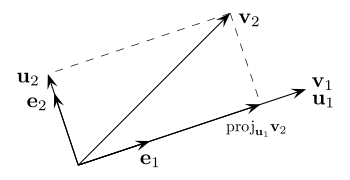
\includegraphics[width=0.8\textwidth]{img/GramSchmidtWiki.png}
    \caption{first two steps of the Gram-Schmidt process}
    \label{fig:Gram-Schmidt-Process-png}
\end{figure}

Given $ k $ nonzero linearly independent vectors $ \mathbf{v}_1, \dots, \mathbf{v}_k $ the
\textbf{Gram-Schmidt} process defines the vectors $ \mathbf{u}_1, \dots, \mathbf{u}_k $
as follows:

\begin{eqarray}
    \mathbf{u}_1 &= \mathbf{v}_1 & \mathbf{e}_1 &= \frac{\mathbf{u}_1}{\norm{\mathbf{u}_1}} \\
    \mathbf{u}_2 &= \mathbf{v}_2 - proj_{\mathbf{u}_1}(\mathbf{v}_2) & \mathbf{e}_2 &= \frac{\mathbf{u}_2}{\norm{\mathbf{u}_2}} \\
    \mathbf{u}_3 &= \mathbf{v}_3 - proj_{\mathbf{u}_1}(\mathbf{v}_3) - proj_{\mathbf{u}_2}(\mathbf{v}_3) & \mathbf{e}_3 &= \frac{\mathbf{u}_3}{\norm{\mathbf{u}_3}} \\
    \quad & \vdots & \quad & \vdots \\
    \mathbf{u}_i &= \mathbf{v}_i - \sum_{j=1}^{i-1} proj_{\mathbf{u}_j}(\mathbf{v}_i) & \mathbf{e}_i &=  \frac{\mathbf{u}_i}{\norm{\mathbf{u}_i}} \\
\end{eqarray}

The sequence $ \mathbf{u}_1, \dots , \mathbf{u}_k $ is the required system of
orthogonal vectors, and the normalised vectors $ \mathbf{e}_1, \dots, \mathbf{e}_k $
form an \textbf{orthonormal set}. The calculation of  $ \mathbf{u}_1, \dots , \mathbf{u}_k $
is known as \textbf{Gram-Schmidt orthogonalisation} and the calculation of sequence
$ \mathbf{e}_1, \dots , \mathbf{e}_k $ is called \textbf{Gram-Schmidt orthonormalisation}.

Python implementation:

\begin{python}
import numpy as np

def GramSchmidtRows(A: np.ndarray, normalise: bool = False):
    """Perform the Gram-Schmidt algorithm on the rows of matrix A so that all
    rows are orthogonalised to the preceding rows"""

    # copy the matrix
    G = A.copy()

    # row to orthogonalise
    for j in range(1, G.shape[0]):
        # the predecessors
        for i in range(j):
            # unit vector representation of preceding row
            unit_row = G[i,:] / np.linalg.norm(G[i,:])
            # projection of current row onto the preceding rows
            G[j,:] -= unit_row * np.dot(G[j,:], unit_row)
        if normalise:
            G[j,:] /= np.linalg.norm(G[j,:])

    return G

def GramSchmidtCols(A: np.ndarray, normalise : bool = False):
    """Perform the Gram-Schmidt algorithm on the columns of matrix A so that all
    columns are orthogonalised to the preceding rows"""

    # copy the matrix
    G = A.copy()

    # column to orthogonalise
    for j in range(1, G.shape[1]):
        # the predecessors
        for i in range(j):
            # unit vector representation of preceding column
            unit_col = G[:,i] / np.linalg.norm(G[:,i])
            # projection of current column onto the preceding columns
            G[:,j] -= unit_col * np.dot(G[:,j], unit_col)
        if normalise:
            G[j,:] /= np.linalg.norm(G[j,:])

    return G
\end{python}


\subsection{Modified Gram-Schmidt process}

The \textbf{Gram-Schmidt orthogonalisation} is prone to \textbf{rounding errors} and
is therefore considered \textbf{numerically unstable}. For the process as described
above it is considered particularly bad.

The \textbf{Gram-Schmidt process} can be stabilised by a small modification, sometimes
referred to as \textbf{modified Gram-Schmidt process} or MGS. This approach
gives the same result as the original formula in exact arithmetic and introdices
smaller errors in finite-precision arithmethic.

Instead of computing the $ \mathbf{u}_i $ as:

\begin{equation}
    \mathbf{u}_i = \mathbf{v}_i - \sum_{j=1}^{i-1} proj_{\mathbf{u}_j}(\mathbf{v}_i)
\end{equation}

it is computed as:

\begin{eqarray}
    \mathbf{u}_{i}^{(1)} &= \mathbf{v}_i - proj_{\mathbf{u}_1}(\mathbf{v}_i) \\
    \mathbf{u}_{i}^{(2)} &= \mathbf{u}_{i}^{(1)} - proj_{\mathbf{u}_2}(\mathbf{u}_{i}^{(1)}) \\
                         & \vdots \\
    \mathbf{u}_{i}^{(i-1)} &= \mathbf{u}_{i}^{(i-2)} - proj_{\mathbf{u}_{i-1}}(\mathbf{u}_{i}^{(i-2)}) \\
    \mathbf{e}_i &= \frac{\mathbf{u}_{i}^{(i-1)}}{\norm{\mathbf{u}_{i}^{(i-1)}}}
\end{eqarray}

Another description would be that the orthogonalisation is performed as a multistep process
where in first step all vectors but first are made orthogonal to the first vectors,
in the second step all vectors but the first two are made orthogonal to the second vector
(already orthogonal to 1st one), and so on untill all are processed.

Python implementation:

\begin{python}
import numpy as np

def ModifiedGramSchmidtRows(A: np.ndarray, normalise: bool = False):
    """Perform the Modified Gram-Schmidt algorithm on the rows of matrix A
    so that all rows are orthogonalised to the preceding rows"""

    # copy the matrix
    G = A.copy()

    # vector to orthogonalise against
    for i in range(G.shape[0]-1):
        # simplify dot product
        unit_row = G[i,:] / np.linalg.norm(G[i,:])
        if normalise:
            G[i,:] = unit_row
        # all later vectors
        for j in range(i+1, G.shape[0]):
            # subtract the projection
            G[j,:] -= unit_row * np.dot(G[j,:], unit_row)

    return G

def ModifiedGramSchmidtCols(A: np.ndarray, normalise: bool = False):
    """Perform the Modified Gram-Schmidt algorithm on the columns of matrix A
    so that all columns are orthogonalised to the preceding rows"""

    # copy the matrix
    G = A.copy()

    # vector to orthogonalise against
    for i in range(G.shape[1]-1):
        # simplify dot product
        unit_col = G[:,i] / np.linalg.norm(G[:,i])
        if normalise:
            G[:,i] = unit_col
        # all later vectors
        for j in range(i+1, G.shape[1]):
            # subtract the projection
            G[:,j] -= unit_col * np.dot(G[:,j], unit_col)

    return G
\end{python}


\section{Factorisation}

\subsection{Cholesky Factorisation}

Cholesky Factorisation is a matrix operation such that a matrix $ \m{A} $ is
decomposed to a multiplication of a lower triangular martrix $ \m{L} $ and its
conjugate transpose $ \m{L}^T $.

The \textbf{Cholesky Factorisation} is applicable to a \textbf{Hermitian},
\textbf{positive definite} matrices.

\begin{equation}
    \m{A} = \m{L} \m{L}^*
\end{equation}

Every Hermitian positive definite matrix (and thus every real-valued symmetric
positive definite matrix) has a unique Cholesky factorisation.

If $ \m{A} $ can be written as $ \m{L} \m{L}^* $ for some invertible $ \m{L} $,
lower triangular or otherwise, then $ \m{A} $ is Hermitian and positive definite.

When $ \m{A} $ is a real matrix (hence symmetric and positive definite), the
factorisation may be written:

\begin{equation}
    \m{A} = \m{L} \m{L}^T
\end{equation}

A Python example of \textit{Cholesky-Banachiewicz} factorisation algorithm:

\begin{python}
import numpy as np

def Cholesky_Banachiewicz(A: np.ndarray) -> np.ndarray:
    """Perform the Choleski factorisation of matrix A such that:

    A = L @ L.T

    where:
        L is lower triangular matrix

    Args:
        A (np.ndarray): a real, symmetric, positive-definite matrix

    Returns:
        (np.ndarray): the result of the decomposition stored as a lower triangular
        matrix.
    """
    L = np.zeros(A.shape, dtype=A.dtype)
    for i in range(A.shape[0]):
        for j in range(i+1):
            sum = 0
            for k in range(j):
                sum += L[i,k] * L[j,k]

            if i == j:
                L[i,j] = np.sqrt(A[i,i] - sum)
            else:
                L[i,j] = 1. / L[j,j] * (A[i,j] - sum)

    return L
\end{python}

And the solution of matrix equation:

\begin{eqarray}
    \mathbf{A} \mathbf{x} &= \mathbf{b} \\
    \mathbf{A} &= \mathbf{L} \mathbf{L}^T \\
    \mathbf{L} \mathbf{L}^T \mathbf{x} &= \mathbf{b} \quad , substitute \quad \mathbf{y} = \mathbf{L}^T \mathbf{x} \\
    \mathbf{L} \mathbf{y} &= \mathbf{b} \quad,\ solve\ using\ forward\ substitution \\
    \mathbf{L}^T \mathbf{x} &= \mathbf{y} \quad,\ solve\ using\ backward\ substitution
\end{eqarray}

the $ \mathbf{b} $ can be either a vector or a matrix.

Python example:

\begin{python}
import numpy as np

def Solve_Triangular(A: np.ndarray, b: np.ndarray, kind="lower") -> np.ndarray:
    """Solve Ax = b using either forward or backward substitution. For lower
    triangular matrix the forward substitution is used, for upper triangular
    matrix the backward substitution is used.
    """
    b = b.copy()
    flatten = False
    if len(b.shape) == 1:
        b = b.reshape(-1,1)
        flatten = True

    m = A.shape[0]
    n = b.shape[1]
    x = np.zeros(b.shape, dtype=b.dtype)

    if kind == "lower":
        for i in range(m):                # rows of A
            x[i,:] = b[i,:]               # perform operations on whole row of b
            for j in range(i):            # columns of A from start to diagonal
                x[i,:] -= A[i,j] * x[j,:] # perform operations on whole row of b
            x[i,:] /= A[i,i]              # divide by the element on the diagonal

    elif kind == "upper":
        for i in reversed(range(m)):      # rows of A from end
            x[i,:] = b[i,:]               # perform operations on whole row of b
            for j in range(i+1, m):       # columns of A from diagonal up to end
                x[i,:] -= A[i,j] * x[j,:] # perform operations on whole row of b
            x[i,:] /= A[i,i]              # divide by the element on the diagonal

    else:
        raise NotImplementedError(f"Substitution for other than 'lower' or 'upper' triangular not implemented: '{kind:s}'.")

    if flatten:
        return x.flatten()
    else:
        return x


def Cholesky_Solve(L: np.ndarray, b: np.ndarray) -> np.ndarray:
    """Solve the matrix equation using results of Cholesky decomposition

        Ax = b
        A = L @ L.T
        L @ L.T @ x = b
        L @ z = b
        L.T @ x = z

    Args:
        L (np.ndarray): a lower triangular matrix from Cholesky decomposition
        b (np.ndarray): right hand side of the equation

    Returns:
        (np.ndarray): the solution on the left hand side
    """
    z = Solve_Triangular(L,   b, "lower")
    x = Solve_Triangular(L.T, z, "upper")
    return x

\end{python}


\subsection{LU Factorisation}

The \textbf{LU factorisation} writes a square matrix as a product of a lower
triangular matrix and an upper triangular matrix:

\begin{equation}
    \m{A} = \m{L} \m{U}
\end{equation}

The factorisation is obtained by applying Gaussian elimination to $ \m{A} $.
The multipliers used to remove the entries below a pivot are stored in
$ \m{L} $, while the resulting upper triangular matrix is $ \m{U} $. Using a
unit diagonal in $ \m{L} $ removes the otherwise arbitrary scaling between the
two factors and gives the \textbf{Doolittle form}:

\begin{equation}
    L_{ii} = 1
\end{equation}

Once the factors are available, the equation $ \m{A}\m{x}=\m{b} $ is solved in
two triangular steps:

\begin{eqarray}
    \m{L}\m{U}\m{x} &= \m{b} \\
    \m{L}\m{y} &= \m{b},\quad solve\ by\ forward\ substitution \\
    \m{U}\m{x} &= \m{y},\quad solve\ by\ backward\ substitution
\end{eqarray}

The factorisation is more expensive than one triangular solution, but it may be
reused for many right hand sides. This is important in finite element analysis,
where the same tangent matrix may be used for several load vectors or for
several operations within one iteration.

\subsubsection{LU Factorisation without pivoting}

For the Doolittle form, comparison of the entries in
$ \m{A}=\m{L}\m{U} $ gives:

\begin{eqarray}
    U_{kj} &= A_{kj} - \sum_{s=1}^{k-1} L_{ks}U_{sj},
    \qquad j=k,\dots,n \\
    L_{ik} &= \frac{1}{U_{kk}}
    \left(A_{ik} - \sum_{s=1}^{k-1}L_{is}U_{sk}\right),
    \qquad i=k+1,\dots,n
\end{eqarray}

The first equation forms row $ k $ of $ \m{U} $. The second equation then forms
column $ k $ of $ \m{L} $. The calculation requires every pivot $ U_{kk} $ to
be nonzero. A nonsingular matrix can nevertheless produce a zero pivot. For
example:

\begin{equation}
    \begin{bmatrix}
        0 & 1 \\
        1 & 0
    \end{bmatrix}
\end{equation}

is nonsingular, but elimination cannot start without exchanging rows. Even when
a pivot is merely very small, division by it can amplify rounding errors.
Factorisation without pivoting is therefore used only when the matrix structure
ensures safe pivots, or when this has been verified separately.

Python implementation:

\begin{python}
import numpy as np


def LU_No_Pivoting(A: np.ndarray,
                   tolerance: float = 1.0e-14):
    """Factorise a square matrix A = L @ U without pivoting.

    L has a unit diagonal. No NumPy linear algebra factorisation or
    solution routine is used.
    """
    A = np.asarray(A)
    n = A.shape[0]

    if A.shape != (n, n):
        raise ValueError("A must be square")

    L = np.eye(n, dtype=A.dtype)
    U = np.zeros_like(A)

    for k in range(n):
        # Form row k of U.
        for j in range(k, n):
            total = 0.0
            for s in range(k):
                total += L[k, s] * U[s, j]
            U[k, j] = A[k, j] - total

        if abs(U[k, k]) <= tolerance:
            raise ZeroDivisionError(
                "zero or numerically small pivot; pivoting is required"
            )

        # Form column k of L.
        for i in range(k + 1, n):
            total = 0.0
            for s in range(k):
                total += L[i, s] * U[s, k]
            L[i, k] = (A[i, k] - total) / U[k, k]

    return L, U


def LU_Solve(L: np.ndarray,
             U: np.ndarray,
             b: np.ndarray) -> np.ndarray:
    """Solve L @ U @ x = b using the triangular solver defined above."""
    y = Solve_Triangular(L, b, kind="lower")
    x = Solve_Triangular(U, y, kind="upper")
    return x
\end{python}

\subsubsection{LU Factorisation with row pivoting}

\textbf{Partial pivoting} exchanges rows before each elimination step. In column
$ k $, the row containing the largest available absolute entry is selected:

\begin{equation}
    p = \underset{i=k,\dots,n}{\operatorname{argmax}}\abs{U_{ik}}
\end{equation}

The corresponding rows are exchanged and the factorisation becomes:

\begin{equation}
    \m{P}\m{A}=\m{L}\m{U}
\end{equation}

where $ \m{P} $ is a permutation matrix. A permutation matrix only changes the
order of equations. It is orthogonal, so that:

\begin{equation}
    \m{P}^{-1}=\m{P}^{T}
\end{equation}

The row exchange avoids division by zero whenever a usable pivot exists in the
current column. Selecting the largest candidate also limits the elimination
multipliers:

\begin{equation}
    \abs{L_{ik}} = \abs{\frac{U_{ik}}{U_{kk}}} \leq 1
\end{equation}

Partial pivoting is the usual general-purpose form of LU factorisation. To solve
$ \m{A}\m{x}=\m{b} $, the right hand side must be permuted in the same way:

\begin{eqarray}
    \m{P}\m{A}\m{x} &= \m{P}\m{b} \\
    \m{L}\m{U}\m{x} &= \m{P}\m{b}
\end{eqarray}

Python implementation:

\begin{python}
import numpy as np


def LU_Partial_Pivoting(A: np.ndarray,
                        tolerance: float = 1.0e-14):
    """Factorise P @ A = L @ U using partial row pivoting."""
    A = np.array(A, copy=True)
    n = A.shape[0]

    if A.shape != (n, n):
        raise ValueError("A must be square")

    U = A.copy()
    L = np.eye(n, dtype=A.dtype)
    P = np.eye(n, dtype=A.dtype)

    for k in range(n - 1):
        # Find the largest available entry in column k.
        pivot = k
        for i in range(k + 1, n):
            if abs(U[i, k]) > abs(U[pivot, k]):
                pivot = i

        if abs(U[pivot, k]) <= tolerance:
            raise ZeroDivisionError("matrix is singular to working precision")

        if pivot != k:
            U[[k, pivot], :] = U[[pivot, k], :]
            P[[k, pivot], :] = P[[pivot, k], :]

            # The already computed part of L belongs to the exchanged rows.
            if k > 0:
                L[[k, pivot], :k] = L[[pivot, k], :k]

        # Gaussian elimination below the pivot.
        for i in range(k + 1, n):
            L[i, k] = U[i, k] / U[k, k]
            U[i, k:] -= L[i, k] * U[k, k:]
            U[i, k] = 0.0

    if abs(U[-1, -1]) <= tolerance:
        raise ZeroDivisionError("matrix is singular to working precision")

    return P, L, U


def LU_Partial_Solve(P: np.ndarray,
                     L: np.ndarray,
                     U: np.ndarray,
                     b: np.ndarray) -> np.ndarray:
    """Solve A @ x = b from P @ A = L @ U."""
    y = Solve_Triangular(L, P @ b, kind="lower")
    x = Solve_Triangular(U, y, kind="upper")
    return x
\end{python}

\subsubsection{LU Factorisation with complete pivoting}

\textbf{Complete pivoting} searches the whole remaining submatrix rather than
only the current column:

\begin{equation}
    (p,q)=\underset{i,j=k,\dots,n}{\operatorname{argmax}}\abs{U_{ij}}
\end{equation}

Both rows and columns are exchanged. The resulting factorisation is:

\begin{equation}
    \m{P}\m{A}\m{Q}=\m{L}\m{U}
\end{equation}

The row permutation $ \m{P} $ reorders equations, while the column permutation
$ \m{Q} $ reorders unknowns. Complete pivoting usually produces smaller element
growth than partial pivoting, but searching the complete trailing submatrix is
more expensive and column permutations complicate bookkeeping. It is therefore
used when additional robustness is more important than the extra work.

For a linear system:

\begin{eqarray}
    \m{P}\m{A}\m{Q} &= \m{L}\m{U} \\
    \m{L}\m{U}\m{Q}^{T}\m{x} &= \m{P}\m{b}
\end{eqarray}

After the triangular solves, the original ordering is restored by
$ \m{x}=\m{Q}\m{y} $.

Python implementation:

\begin{python}
import numpy as np


def LU_Complete_Pivoting(A: np.ndarray,
                         tolerance: float = 1.0e-14):
    """Factorise P @ A @ Q = L @ U using complete pivoting."""
    A = np.array(A, copy=True)
    n = A.shape[0]

    if A.shape != (n, n):
        raise ValueError("A must be square")

    U = A.copy()
    L = np.eye(n, dtype=A.dtype)
    P = np.eye(n, dtype=A.dtype)
    Q = np.eye(n, dtype=A.dtype)

    for k in range(n - 1):
        pivot_row = k
        pivot_col = k
        pivot_value = abs(U[k, k])

        for i in range(k, n):
            for j in range(k, n):
                if abs(U[i, j]) > pivot_value:
                    pivot_row = i
                    pivot_col = j
                    pivot_value = abs(U[i, j])

        if pivot_value <= tolerance:
            raise ZeroDivisionError("matrix is singular to working precision")

        if pivot_row != k:
            U[[k, pivot_row], :] = U[[pivot_row, k], :]
            P[[k, pivot_row], :] = P[[pivot_row, k], :]
            if k > 0:
                L[[k, pivot_row], :k] = L[[pivot_row, k], :k]

        if pivot_col != k:
            U[:, [k, pivot_col]] = U[:, [pivot_col, k]]
            Q[:, [k, pivot_col]] = Q[:, [pivot_col, k]]

        for i in range(k + 1, n):
            L[i, k] = U[i, k] / U[k, k]
            U[i, k:] -= L[i, k] * U[k, k:]
            U[i, k] = 0.0

    if abs(U[-1, -1]) <= tolerance:
        raise ZeroDivisionError("matrix is singular to working precision")

    return P, L, U, Q


def LU_Complete_Solve(P: np.ndarray,
                      L: np.ndarray,
                      U: np.ndarray,
                      Q: np.ndarray,
                      b: np.ndarray) -> np.ndarray:
    """Solve A @ x = b from P @ A @ Q = L @ U."""
    z = Solve_Triangular(L, P @ b, kind="lower")
    y = Solve_Triangular(U, z, kind="upper")
    x = Q @ y
    return x
\end{python}

\subsection{QR Factorisation}

The \textbf{QR factorisation} writes an $ m\times n $ matrix with
$ m\geq n $ as:

\begin{equation}
    \m{A}=\m{Q}\m{R}
\end{equation}

where the columns of $ \m{Q} $ are orthonormal and $ \m{R} $ is upper
triangular:

\begin{equation}
    \m{Q}^{*}\m{Q}=\m{I}
\end{equation}

In the \textbf{thin QR factorisation}, $ \m{Q} $ has size $ m\times n $ and
$ \m{R} $ has size $ n\times n $. In the full factorisation, $ \m{Q} $ is
$ m\times m $ and $ \m{R} $ is $ m\times n $.

Because multiplication by an orthogonal matrix does not change the Euclidean
norm, QR factorisation transforms a least-squares problem without squaring its
condition number:

\begin{eqarray}
    \underset{\m{x}}{\operatorname{minimise}}\norm{\m{A}\m{x}-\m{b}}_2
    &=
    \underset{\m{x}}{\operatorname{minimise}}
    \norm{\m{Q}^{*}\m{A}\m{x}-\m{Q}^{*}\m{b}}_2 \\
    &=
    \underset{\m{x}}{\operatorname{minimise}}
    \norm{\m{R}\m{x}-\m{Q}^{*}\m{b}}_2
\end{eqarray}

This is numerically preferable to forming the normal equations
$ \m{A}^{*}\m{A}\m{x}=\m{A}^{*}\m{b} $.

\subsubsection{QR Factorisation using Gram-Schmidt algorithm}

Gram-Schmidt orthogonalisation of the columns of $ \m{A} $ gives
$ \m{Q} $. Let $ \m{a}_j $ be column $ j $ of $ \m{A} $. Then:

\begin{eqarray}
    R_{ij} &= \m{q}_i^{*}\m{a}_j, \qquad i<j \\
    \m{v}_j &= \m{a}_j-\sum_{i=1}^{j-1}R_{ij}\m{q}_i \\
    R_{jj} &= \norm{\m{v}_j}_2 \\
    \m{q}_j &= \frac{\m{v}_j}{R_{jj}}
\end{eqarray}

The coefficients removed from column $ j $ form column $ j $ of
$ \m{R} $. If $ R_{jj}=0 $, the new column is linearly dependent on the
previous columns and a full-rank thin QR factorisation does not exist.

The following code uses the modified ordering of the Gram-Schmidt operations,
which is less sensitive to rounding errors than evaluating all projections from
the original column at once.

\begin{python}
import numpy as np


def Vector_Norm(x: np.ndarray) -> float:
    """Euclidean norm without using numpy.linalg."""
    value = np.dot(np.conjugate(x), x)
    return float(np.sqrt(np.real(value)))


def QR_Gram_Schmidt(A: np.ndarray,
                    tolerance: float = 1.0e-14):
    """Compute the thin QR factorisation A = Q @ R."""
    A = np.asarray(A)
    m, n = A.shape

    if m < n:
        raise ValueError("the example assumes m >= n")

    Q = np.zeros((m, n), dtype=A.dtype)
    R = np.zeros((n, n), dtype=A.dtype)

    for j in range(n):
        v = A[:, j].copy()

        for i in range(j):
            R[i, j] = np.dot(np.conjugate(Q[:, i]), v)
            v -= R[i, j] * Q[:, i]

        R[j, j] = Vector_Norm(v)
        if R[j, j] <= tolerance:
            raise ValueError("columns of A are linearly dependent")

        Q[:, j] = v / R[j, j]

    return Q, R
\end{python}

\subsubsection{QR Factorisation using Givens rotations}

A \textbf{Givens rotation} acts only in a plane spanned by two coordinate axes.
For real numbers $ a $ and $ b $, choose:

\begin{equation}
    c=\frac{a}{r},\qquad s=\frac{b}{r},\qquad
    r=\sqrt{a^2+b^2}
\end{equation}

and define:

\begin{equation}
    \m{G}=
    \begin{bmatrix}
        c & s \\
        -s & c
    \end{bmatrix}
\end{equation}

Then:

\begin{equation}
    \m{G}
    \begin{bmatrix}
        a \\
        b
    \end{bmatrix}
    =
    \begin{bmatrix}
        r \\
        0
    \end{bmatrix}
\end{equation}

Embedding this $ 2\times2 $ block into an identity matrix allows one entry below
the diagonal of $ \m{A} $ to be removed without changing the other rows. A
sequence of rotations gives:

\begin{equation}
    \m{G}_p\cdots\m{G}_2\m{G}_1\m{A}=\m{R}
\end{equation}

and therefore:

\begin{equation}
    \m{A}=\m{Q}\m{R},\qquad
    \m{Q}=\m{G}_1^{T}\m{G}_2^{T}\cdots\m{G}_p^{T}
\end{equation}

Givens rotations are especially useful when the matrix is sparse or when only a
small number of new entries must be eliminated, because each rotation modifies
only two rows.

Python implementation:

\begin{python}
import numpy as np


def Givens_Parameters(a: float, b: float):
    """Return c and s so [[c,s],[-s,c]] @ [a,b] = [r,0]."""
    r = float(np.hypot(abs(a), abs(b)))
    if r == 0.0:
        return 1.0, 0.0
    return a / r, b / r


def QR_Givens(A: np.ndarray,
              tolerance: float = 1.0e-14):
    """Compute A = Q @ R using real Givens rotations."""
    R = np.array(A, dtype=float, copy=True)
    m, n = R.shape
    Q = np.eye(m)

    for j in range(min(m, n)):
        # Work upwards so each rotation removes one entry in column j.
        for i in reversed(range(j + 1, m)):
            if abs(R[i, j]) <= tolerance:
                continue

            c, s = Givens_Parameters(R[i - 1, j], R[i, j])

            row_1 = R[i - 1, j:].copy()
            row_2 = R[i, j:].copy()
            R[i - 1, j:] = c * row_1 + s * row_2
            R[i, j:] = -s * row_1 + c * row_2

            # Q <- Q @ G.T, applied only to two columns.
            col_1 = Q[:, i - 1].copy()
            col_2 = Q[:, i].copy()
            Q[:, i - 1] = c * col_1 + s * col_2
            Q[:, i] = -s * col_1 + c * col_2

    R[abs(R) < tolerance] = 0.0
    return Q, R
\end{python}

\subsubsection{QR Factorisation using Householder reflections}

A \textbf{Householder reflection} maps a vector onto a coordinate axis in one
operation. For a unit vector $ \m{v} $:

\begin{equation}
    \m{H}=\m{I}-2\m{v}\m{v}^{*}
\end{equation}

The matrix is Hermitian and unitary:

\begin{equation}
    \m{H}^{*}=\m{H},\qquad \m{H}^{*}\m{H}=\m{I}
\end{equation}

For a column segment $ \m{x} $, the vector $ \m{v} $ is selected so that:

\begin{equation}
    \m{H}\m{x}=-\operatorname{sign}(x_1)\norm{\m{x}}_2\m{e}_1
\end{equation}

The sign is chosen to avoid subtracting nearly equal numbers while constructing
$ \m{v} $. Each reflection removes all entries below one diagonal position. A
matrix with $ n $ columns therefore needs at most $ n $ reflections. Compared
with Gram-Schmidt, Householder QR usually gives better numerical orthogonality
and is the standard dense-matrix method.

Python implementation:

\begin{python}
import numpy as np


def Householder_Vector(x: np.ndarray,
                       tolerance: float = 1.0e-14):
    """Return a unit vector v defining H = I - 2 v v*."""
    x = np.asarray(x)
    norm_x = Vector_Norm(x)

    if norm_x <= tolerance:
        return np.zeros_like(x), False

    phase = 1.0 if x[0] == 0.0 else x[0] / abs(x[0])
    v = x.copy()
    v[0] += phase * norm_x

    norm_v = Vector_Norm(v)
    if norm_v <= tolerance:
        return np.zeros_like(x), False

    return v / norm_v, True


def QR_Householder(A: np.ndarray,
                   tolerance: float = 1.0e-14):
    """Compute the full factorisation A = Q @ R."""
    R = np.array(A, copy=True)
    m, n = R.shape
    Q = np.eye(m, dtype=R.dtype)

    for k in range(min(m, n)):
        v, active = Householder_Vector(R[k:, k], tolerance)
        if not active:
            continue

        # R <- H @ R, applied only to the active trailing block.
        projection = np.dot(np.conjugate(v), R[k:, k:])
        R[k:, k:] -= 2.0 * np.outer(v, projection)

        # Q <- Q @ H. H is Hermitian, hence H* = H.
        projection = np.dot(Q[:, k:], v)
        Q[:, k:] -= 2.0 * np.outer(projection, np.conjugate(v))

    R[abs(R) < tolerance] = 0.0
    return Q, R
\end{python}

\subsubsection{QR Factorisation using Householder reflections with column pivoting}

If columns of $ \m{A} $ are nearly linearly dependent, a small diagonal value in
$ \m{R} $ may occur before the independent directions have been processed.
\textbf{Column-pivoted QR} chooses at every step the remaining column with the
largest residual norm. The factorisation is written:

\begin{equation}
    \m{A}\m{P}=\m{Q}\m{R}
\end{equation}

where $ \m{P} $ is a column permutation matrix. The diagonal entries of
$ \m{R} $ then tend to decrease in magnitude. This reveals the numerical rank:

\begin{equation}
    \abs{R_{11}}\geq\abs{R_{22}}\geq\dots
\end{equation}

The relation is not guaranteed to be exact for every matrix, but the diagonal
usually separates well-resolved and nearly dependent directions. This makes
pivoted QR useful for rank detection, least-squares problems and selecting
independent interface or measurement coordinates.

Python implementation:

\begin{python}
import numpy as np


def QR_Householder_Pivoting(A: np.ndarray,
                            tolerance: float = 1.0e-14):
    """Compute A @ P = Q @ R using Householder column pivoting."""
    R = np.array(A, copy=True)
    m, n = R.shape
    Q = np.eye(m, dtype=R.dtype)
    P = np.eye(n, dtype=R.dtype)

    for k in range(min(m, n)):
        # Recompute the residual column norms for clarity.
        pivot = k
        largest_norm_squared = -1.0
        for j in range(k, n):
            value = np.dot(np.conjugate(R[k:, j]), R[k:, j])
            norm_squared = float(np.real(value))
            if norm_squared > largest_norm_squared:
                largest_norm_squared = norm_squared
                pivot = j

        if pivot != k:
            R[:, [k, pivot]] = R[:, [pivot, k]]
            P[:, [k, pivot]] = P[:, [pivot, k]]

        v, active = Householder_Vector(R[k:, k], tolerance)
        if not active:
            continue

        projection = np.dot(np.conjugate(v), R[k:, k:])
        R[k:, k:] -= 2.0 * np.outer(v, projection)

        projection = np.dot(Q[:, k:], v)
        Q[:, k:] -= 2.0 * np.outer(projection, np.conjugate(v))

    R[abs(R) < tolerance] = 0.0
    return Q, R, P
\end{python}

\subsection{Conversion to Hessenberg form using Givens rotations}

The QR factorisation applies orthogonal transformations from the left and changes
$ \m{A} $ into an upper triangular matrix. An eigenvalue problem requires a
\textbf{similarity transformation}, because similarity preserves eigenvalues:

\begin{equation}
    \m{H}=\m{Q}^{*}\m{A}\m{Q}
\end{equation}

An \textbf{upper Hessenberg matrix} has zeros below its first subdiagonal:

\begin{equation}
    H_{ij}=0 \qquad \text{for}\quad i>j+1
\end{equation}

A Givens rotation is first applied from the left to remove one entry below the
first subdiagonal and then from the right with its transpose. The right
multiplication is essential: without it the operation would not be a similarity
transformation. Repeating this process gives a Hessenberg matrix with the same
eigenvalues as $ \m{A} $. If $ \m{A} $ is symmetric, symmetry is preserved and
the Hessenberg matrix is tridiagonal.

Python implementation:

\begin{python}
import numpy as np


def Hessenberg_Givens(A: np.ndarray,
                      tolerance: float = 1.0e-14):
    """Compute H = Q.T @ A @ Q using real Givens rotations."""
    H = np.array(A, dtype=float, copy=True)
    n = H.shape[0]

    if H.shape != (n, n):
        raise ValueError("A must be square")

    Q = np.eye(n)

    for k in range(n - 2):
        for i in reversed(range(k + 2, n)):
            if abs(H[i, k]) <= tolerance:
                continue

            c, s = Givens_Parameters(H[i - 1, k], H[i, k])

            # H <- G @ H: rotate rows i-1 and i.
            row_1 = H[i - 1, :].copy()
            row_2 = H[i, :].copy()
            H[i - 1, :] = c * row_1 + s * row_2
            H[i, :] = -s * row_1 + c * row_2

            # H <- H @ G.T: rotate the matching columns.
            col_1 = H[:, i - 1].copy()
            col_2 = H[:, i].copy()
            H[:, i - 1] = c * col_1 + s * col_2
            H[:, i] = -s * col_1 + c * col_2

            # Q <- Q @ G.T.
            col_1 = Q[:, i - 1].copy()
            col_2 = Q[:, i].copy()
            Q[:, i - 1] = c * col_1 + s * col_2
            Q[:, i] = -s * col_1 + c * col_2

    H[abs(H) < tolerance] = 0.0
    return Q, H
\end{python}

\subsection{Conversion to Hessenberg form using Householder reflections}

A Householder reflection can remove a complete column segment in one operation.
At step $ k $, a reflector is constructed from:

\begin{equation}
    \m{x}=\m{A}_{k+1:n,k}
\end{equation}

and embedded into the identity matrix:

\begin{equation}
    \widehat{\m{H}}_k=
    \begin{bmatrix}
        \m{I}_{k} & \m{0} \\
        \m{0} & \m{H}_k
    \end{bmatrix}
\end{equation}

The similarity update is:

\begin{equation}
    \m{A}_{k+1}=\widehat{\m{H}}_k^{*}\m{A}_k\widehat{\m{H}}_k
\end{equation}

Since a Householder reflector is Hermitian, its conjugate transpose is the
reflector itself. For dense matrices this method requires fewer transformations
than the Givens method and is normally preferred. Again, a symmetric matrix is
reduced to symmetric tridiagonal form.

Python implementation:

\begin{python}
import numpy as np


def Hessenberg_Householder(A: np.ndarray,
                           tolerance: float = 1.0e-14):
    """Compute H = Q* @ A @ Q by Householder similarity transforms."""
    H = np.array(A, copy=True)
    n = H.shape[0]

    if H.shape != (n, n):
        raise ValueError("A must be square")

    Q = np.eye(n, dtype=H.dtype)

    for k in range(n - 2):
        v, active = Householder_Vector(H[k + 1:, k], tolerance)
        if not active:
            continue

        # Left multiplication by the embedded reflector.
        projection = np.dot(np.conjugate(v), H[k + 1:, :])
        H[k + 1:, :] -= 2.0 * np.outer(v, projection)

        # Right multiplication by the same reflector.
        projection = np.dot(H[:, k + 1:], v)
        H[:, k + 1:] -= 2.0 * np.outer(
            projection, np.conjugate(v)
        )

        # Accumulate Q.
        projection = np.dot(Q[:, k + 1:], v)
        Q[:, k + 1:] -= 2.0 * np.outer(
            projection, np.conjugate(v)
        )

    H[abs(H) < tolerance] = 0.0
    return Q, H
\end{python}

\subsection{Jacobi similarity rotations}

A \textbf{Jacobi rotation} is a symmetric plane rotation used on both sides of a
real symmetric matrix:

\begin{equation}
    \m{A}_{new}=\m{J}^{T}\m{A}\m{J}
\end{equation}

For selected indices $ p $ and $ q $, the nontrivial part of $ \m{J} $ is:

\begin{equation}
    \begin{bmatrix}
        c & -s \\
        s & c
    \end{bmatrix}
\end{equation}

The angle can be selected so that $ A_{pq} $ and $ A_{qp} $ become zero. Unlike
Householder Hessenberg reduction, however, a later Jacobi rotation can recreate
entries that an earlier rotation removed. Jacobi rotations are therefore not a
finite general-purpose Hessenberg-reduction algorithm. Their natural use is to
reduce a symmetric matrix directly towards diagonal form, as described in the
next subsection.

A single Jacobi similarity step is useful for understanding the operation:

\begin{python}
import numpy as np


def Jacobi_Rotation(A: np.ndarray, p: int, q: int):
    """Apply one Jacobi similarity rotation to a real symmetric matrix."""
    A = np.array(A, dtype=float, copy=True)
    n = A.shape[0]

    if A.shape != (n, n):
        raise ValueError("A must be square")
    if p == q:
        return A, np.eye(n)

    theta = 0.5 * np.arctan2(
        2.0 * A[p, q], A[p, p] - A[q, q]
    )
    c = float(np.cos(theta))
    s = float(np.sin(theta))

    J = np.eye(n)
    J[p, p] = c
    J[q, q] = c
    J[p, q] = -s
    J[q, p] = s

    return J.T @ A @ J, J
\end{python}

\subsection{Jacobi rotations to diagonal matrix}

For a real symmetric matrix, repeated Jacobi rotations reduce the off-diagonal
entries while preserving symmetry and eigenvalues. When the process converges:

\begin{equation}
    \m{D}=\m{V}^{T}\m{A}\m{V}
\end{equation}

where $ \m{D} $ is diagonal and the columns of $ \m{V} $ are orthonormal
eigenvectors. The diagonal entries of $ \m{D} $ are the eigenvalues.

A simple strategy selects the largest off-diagonal entry in every iteration:

\begin{equation}
    (p,q)=\underset{p<q}{\operatorname{argmax}}\abs{A_{pq}}
\end{equation}

The rotation angle is obtained from:

\begin{equation}
    \tan(2\theta)=\frac{2A_{pq}}{A_{pp}-A_{qq}}
\end{equation}

Using $ \operatorname{atan2} $ avoids an explicit division and preserves the
correct quadrant. The method is easy to understand and produces accurate
eigenvectors, but each rotation changes rows and columns of a dense matrix. It
is therefore mainly useful for small or medium symmetric problems and as a
reference implementation.

Python implementation:

\begin{python}
import numpy as np


def Jacobi_Eigenvalue(A: np.ndarray,
                      tolerance: float = 1.0e-12,
                      max_iterations: int = 10000):
    """Diagonalise a real symmetric matrix with Jacobi rotations."""
    D = np.array(A, dtype=float, copy=True)
    n = D.shape[0]

    if D.shape != (n, n):
        raise ValueError("A must be square")

    V = np.eye(n)

    for iteration in range(max_iterations):
        # Locate the largest off-diagonal entry.
        p = 0
        q = 1
        largest = 0.0
        for i in range(n - 1):
            for j in range(i + 1, n):
                if abs(D[i, j]) > largest:
                    largest = abs(D[i, j])
                    p = i
                    q = j

        if largest <= tolerance:
            break

        theta = 0.5 * np.arctan2(
            2.0 * D[p, q], D[p, p] - D[q, q]
        )
        c = float(np.cos(theta))
        s = float(np.sin(theta))

        J = np.eye(n)
        J[p, p] = c
        J[q, q] = c
        J[p, q] = -s
        J[q, p] = s

        D = J.T @ D @ J
        V = V @ J

        # Remove round-off remaining in the selected location.
        D[p, q] = 0.0
        D[q, p] = 0.0
    else:
        raise RuntimeError("Jacobi iteration did not converge")

    eigenvalues = np.diag(D).copy()
    return eigenvalues, V
\end{python}

\subsection{Arnoldi algorithm}

The \textbf{Arnoldi algorithm} constructs an orthonormal basis of a Krylov
subspace for a general square matrix:

\begin{equation}
    \mathcal{K}_m(\m{A},\m{b})=
    \operatorname{span}\left\{
        \m{b},\m{A}\m{b},\dots,\m{A}^{m-1}\m{b}
    \right\}
\end{equation}

Directly forming the powers of $ \m{A} $ would rapidly produce nearly dependent
vectors. Arnoldi instead multiplies the newest basis vector by $ \m{A} $ and
orthogonalises the result against all preceding vectors. This gives:

\begin{equation}
    \m{A}\m{V}_m=\m{V}_{m+1}\overline{\m{H}}_m
\end{equation}

where $ \m{V}_{m+1} $ has orthonormal columns and
$ \overline{\m{H}}_m $ is upper Hessenberg. The projected matrix:

\begin{equation}
    \m{H}_m=\m{V}_m^{*}\m{A}\m{V}_m
\end{equation}

is small. Its eigenvalues are called \textbf{Ritz values} and approximate
selected eigenvalues of $ \m{A} $. The same relation is the basis of GMRES for
linear systems.

If the new vector has zero norm, the Krylov subspace has become invariant under
$ \m{A} $. This is called a \textbf{happy breakdown}: no further basis vectors
are required in exact arithmetic.

Python implementation:

\begin{python}
import numpy as np


def Arnoldi(A: np.ndarray,
            b: np.ndarray,
            steps: int,
            tolerance: float = 1.0e-14):
    """Construct an Arnoldi basis and upper Hessenberg projection."""
    A = np.asarray(A)
    b = np.asarray(b)
    n = A.shape[0]
    m = min(steps, n)
    dtype = np.result_type(A, b)

    V = np.zeros((n, m + 1), dtype=dtype)
    H = np.zeros((m + 1, m), dtype=dtype)

    beta = Vector_Norm(b)
    if beta <= tolerance:
        raise ValueError("the starting vector must be nonzero")

    V[:, 0] = b / beta
    used_steps = m

    for j in range(m):
        w = A @ V[:, j]

        # Modified Gram-Schmidt orthogonalisation.
        for i in range(j + 1):
            H[i, j] = np.dot(np.conjugate(V[:, i]), w)
            w -= H[i, j] * V[:, i]

        H[j + 1, j] = Vector_Norm(w)

        if H[j + 1, j] <= tolerance:
            used_steps = j + 1
            break

        V[:, j + 1] = w / H[j + 1, j]

    return (
        V[:, :used_steps + 1],
        H[:used_steps + 1, :used_steps]
    )
\end{python}

\subsection{Lanczos algorithm}

For a Hermitian matrix, the Arnoldi projected matrix is also Hermitian. A matrix
that is both Hermitian and upper Hessenberg must be tridiagonal. This removes the
need to orthogonalise against every preceding vector and gives the
\textbf{Lanczos three-term recurrence}:

\begin{eqarray}
    \m{w}_j &= \m{A}\m{v}_j-\beta_{j-1}\m{v}_{j-1} \\
    \alpha_j &= \m{v}_j^{*}\m{w}_j \\
    \m{w}_j &\leftarrow \m{w}_j-\alpha_j\m{v}_j \\
    \beta_j &= \norm{\m{w}_j}_2 \\
    \m{v}_{j+1} &= \frac{\m{w}_j}{\beta_j}
\end{eqarray}

The resulting relation is:

\begin{equation}
    \m{A}\m{V}_m=\m{V}_m\m{T}_m+
    \beta_m\m{v}_{m+1}\m{e}_m^{T}
\end{equation}

where $ \m{T}_m $ is real symmetric tridiagonal for a real symmetric
$ \m{A} $. Lanczos is well suited to large sparse structural eigenvalue
problems because it requires only matrix-vector products and stores a limited
number of vectors.

In exact arithmetic, the three-term recurrence preserves orthogonality. In
finite precision, converged directions may reappear and produce duplicate Ritz
values. The example therefore includes optional full reorthogonalisation. This
increases the cost but makes the educational implementation reliable.

Python implementation:

\begin{python}
import numpy as np


def Lanczos(A: np.ndarray,
            b: np.ndarray,
            steps: int,
            tolerance: float = 1.0e-14,
            reorthogonalise: bool = True):
    """Construct a Lanczos basis and symmetric tridiagonal projection."""
    A = np.asarray(A)
    b = np.asarray(b)
    n = A.shape[0]
    m = min(steps, n)
    dtype = np.result_type(A, b)

    V = np.zeros((n, m), dtype=dtype)
    alpha = np.zeros(m)
    beta = np.zeros(max(m - 1, 0))

    norm_b = Vector_Norm(b)
    if norm_b <= tolerance:
        raise ValueError("the starting vector must be nonzero")

    v = b / norm_b
    v_previous = np.zeros_like(v)
    beta_previous = 0.0
    used_steps = m

    for j in range(m):
        V[:, j] = v
        w = A @ v - beta_previous * v_previous

        alpha[j] = float(np.real(np.dot(np.conjugate(v), w)))
        w -= alpha[j] * v

        if reorthogonalise:
            for i in range(j + 1):
                coefficient = np.dot(np.conjugate(V[:, i]), w)
                w -= coefficient * V[:, i]

        if j == m - 1:
            break

        beta[j] = Vector_Norm(w)
        if beta[j] <= tolerance:
            used_steps = j + 1
            break

        v_previous = v
        v = w / beta[j]
        beta_previous = beta[j]

    T = np.diag(alpha[:used_steps])
    if used_steps > 1:
        T += np.diag(beta[:used_steps - 1], 1)
        T += np.diag(beta[:used_steps - 1], -1)

    return V[:, :used_steps], T
\end{python}

\subsection{Schur algorithm}

Every square complex matrix has a \textbf{Schur decomposition}:

\begin{equation}
    \m{A}=\m{Z}\m{T}\m{Z}^{*}
\end{equation}

where $ \m{Z} $ is unitary and $ \m{T} $ is upper triangular. The eigenvalues of
$ \m{A} $ appear on the diagonal of $ \m{T} $. For real arithmetic, a real
matrix is generally reduced to \textbf{real Schur form}, which is upper
quasi-triangular and may contain $ 2\times2 $ diagonal blocks representing
complex-conjugate eigenvalue pairs.

The QR algorithm first reduces $ \m{A} $ to Hessenberg form and then repeatedly
performs shifted QR steps:

\begin{eqarray}
    \m{H}_k-\mu_k\m{I} &= \m{Q}_k\m{R}_k \\
    \m{H}_{k+1} &= \m{R}_k\m{Q}_k+\mu_k\m{I}
\end{eqarray}

Since:

\begin{equation}
    \m{H}_{k+1}=\m{Q}_k^{*}\m{H}_k\m{Q}_k
\end{equation}

all iterates are similar and have the same eigenvalues. The shift
$ \mu_k $ accelerates convergence. When a subdiagonal entry becomes small, the
corresponding eigenvalue is \textbf{deflated} and the iteration continues on the
remaining leading block.

The following educational implementation converts the matrix to complex
arithmetic. It therefore converges to triangular complex Schur form even when
the original real matrix has complex eigenvalues. Production eigensolvers use
more sophisticated double shifts, aggressive deflation and carefully blocked
operations.

\begin{python}
import numpy as np


def Schur_QR(A: np.ndarray,
             tolerance: float = 1.0e-10,
             max_iterations: int = 5000):
    """Compute a simple complex Schur form using shifted QR iteration.

    This example reuses Hessenberg_Householder and QR_Householder.
    """
    A = np.array(A, dtype=complex, copy=True)
    n = A.shape[0]

    if A.shape != (n, n):
        raise ValueError("A must be square")

    Z, H = Hessenberg_Householder(A, tolerance * 0.01)
    active = n
    iterations = 0

    while active > 1:
        scale = (
            abs(H[active - 2, active - 2])
            + abs(H[active - 1, active - 1])
            + 1.0
        )

        if abs(H[active - 1, active - 2]) <= tolerance * scale:
            H[active - 1, active - 2] = 0.0
            active -= 1
            continue

        if iterations >= max_iterations:
            raise RuntimeError("shifted QR iteration did not converge")

        # A simple Rayleigh shift from the last diagonal entry.
        shift = H[active - 1, active - 1]
        shifted = (
            H[:active, :active]
            - shift * np.eye(active, dtype=complex)
        )
        Q_step, R_step = QR_Householder(
            shifted, tolerance * 0.01
        )

        # Apply the block similarity transformation to the whole matrix.
        H[:active, :] = np.conjugate(Q_step).T @ H[:active, :]
        H[:, :active] = H[:, :active] @ Q_step
        Z[:, :active] = Z[:, :active] @ Q_step

        iterations += 1

    H[abs(H) < tolerance] = 0.0
    return Z, H
\end{python}

\subsection{Singular Value Decomposition (SVD)}

For any real or complex $ m\times n $ matrix, the \textbf{singular value
decomposition} is:

\begin{equation}
    \m{A}=\m{U}\m{\Sigma}\m{V}^{*}
\end{equation}

The columns of $ \m{U} $ and $ \m{V} $ are orthonormal. The diagonal entries of
$ \m{\Sigma} $ are nonnegative singular values:

\begin{equation}
    \sigma_1\geq\sigma_2\geq\dots\geq0
\end{equation}

The right singular vectors are eigenvectors of $ \m{A}^{*}\m{A} $, while the
left singular vectors are eigenvectors of $ \m{A}\m{A}^{*} $:

\begin{eqarray}
    \m{A}^{*}\m{A}\m{v}_i &= \sigma_i^2\m{v}_i \\
    \m{A}\m{A}^{*}\m{u}_i &= \sigma_i^2\m{u}_i \\
    \m{A}\m{v}_i &= \sigma_i\m{u}_i
\end{eqarray}

The SVD exposes matrix rank, null spaces and conditioning. It also gives the best
rank-$ r $ approximation in the Euclidean and Frobenius norms:

\begin{equation}
    \m{A}_r=\sum_{i=1}^{r}\sigma_i\m{u}_i\m{v}_i^{*}
\end{equation}

The algorithms below form $ \m{A}^{*}\m{A} $ implicitly through repeated
matrix-vector or matrix-block products. This is useful for explaining the
relation to eigenvalue iteration, but it squares the condition number and is
not the preferred production SVD algorithm. Robust libraries use bidiagonal
reduction followed by specialised iterations.

\subsubsection{SVD using Power Iteration}

Power iteration applied to $ \m{A}^{*}\m{A} $ converges to the dominant right
singular vector:

\begin{equation}
    \m{v}^{(k+1)}=
    \frac{\m{A}^{*}\m{A}\m{v}^{(k)}}
    {\norm{\m{A}^{*}\m{A}\m{v}^{(k)}}_2}
\end{equation}

After convergence:

\begin{eqarray}
    \sigma &= \norm{\m{A}\m{v}}_2 \\
    \m{u} &= \frac{\m{A}\m{v}}{\sigma}
\end{eqarray}

The rank-one part is then removed:

\begin{equation}
    \m{A}\leftarrow\m{A}-\sigma\m{u}\m{v}^{*}
\end{equation}

and the iteration is repeated for the next singular triplet. This
\textbf{deflation} is simple but accumulated rounding errors can reduce
orthogonality, especially for clustered or repeated singular values.

Python implementation:

\begin{python}
import numpy as np


def SVD_Power(A: np.ndarray,
              rank: int = None,
              tolerance: float = 1.0e-10,
              max_iterations: int = 10000):
    """Approximate a thin SVD by power iteration and rank-one deflation."""
    B = np.array(A, dtype=float, copy=True)
    m, n = B.shape
    maximum_rank = min(m, n)
    r = maximum_rank if rank is None else min(rank, maximum_rank)

    U = np.zeros((m, r))
    singular_values = np.zeros(r)
    V = np.zeros((n, r))
    used_rank = r

    for k in range(r):
        # A deterministic nonzero initial vector.
        v = np.arange(1, n + 1, dtype=float) + k
        v /= Vector_Norm(v)

        for iteration in range(max_iterations):
            w = B.T @ (B @ v)
            norm_w = Vector_Norm(w)

            if norm_w <= tolerance:
                used_rank = k
                break

            v_new = w / norm_w

            # The sign of a singular vector is arbitrary.
            same_sign = Vector_Norm(v_new - v)
            opposite_sign = Vector_Norm(v_new + v)
            v = v_new

            if min(same_sign, opposite_sign) <= tolerance:
                break
        else:
            raise RuntimeError("power iteration did not converge")

        if used_rank == k:
            break

        Av = B @ v
        sigma = Vector_Norm(Av)
        if sigma <= tolerance:
            used_rank = k
            break

        u = Av / sigma
        U[:, k] = u
        singular_values[k] = sigma
        V[:, k] = v

        # Remove the converged rank-one contribution.
        B -= sigma * np.outer(u, v)

    return (
        U[:, :used_rank],
        singular_values[:used_rank],
        V[:, :used_rank].T
    )
\end{python}

\subsubsection{SVD using QR (orthogonal) Iteration}

Power iteration finds one direction at a time. \textbf{Orthogonal iteration}
propagates a complete subspace. Starting with an orthonormal matrix
$ \m{Q}^{(0)} $, repeat:

\begin{eqarray}
    \m{Y}^{(k)} &= \m{A}^{*}\m{A}\m{Q}^{(k)} \\
    \m{Y}^{(k)} &= \m{Q}^{(k+1)}\m{R}^{(k+1)}
\end{eqarray}

The QR factorisation prevents all columns from collapsing onto the dominant
singular vector. After convergence, each column $ \m{q}_i $ approximates a right
singular vector. The corresponding left vector and singular value are:

\begin{eqarray}
    \sigma_i &= \norm{\m{A}\m{q}_i}_2 \\
    \m{u}_i &= \frac{\m{A}\m{q}_i}{\sigma_i}
\end{eqarray}

Convergence depends on separation between singular values. Repeated singular
values define an invariant subspace rather than unique individual vectors; any
orthonormal basis of that subspace is valid.

Python implementation:

\begin{python}
import numpy as np


def SVD_Orthogonal_Iteration(A: np.ndarray,
                             tolerance: float = 1.0e-10,
                             max_iterations: int = 10000):
    """Approximate a thin SVD using block orthogonal iteration.

    The example reuses QR_Householder and does not call numpy.linalg.
    """
    A = np.array(A, dtype=float, copy=True)
    m, n = A.shape
    r = min(m, n)

    # Construct a deterministic full-rank starting block.
    seed = np.empty((n, r))
    for i in range(n):
        for j in range(r):
            seed[i, j] = 1.0 / (1.0 + i + j)
            if i == j:
                seed[i, j] += 1.0

    Q, unused_R = QR_Householder(seed)
    Q = Q[:, :r]

    for iteration in range(max_iterations):
        Y = A.T @ (A @ Q)
        Q_new, unused_R = QR_Householder(Y)
        Q_new = Q_new[:, :r]

        # Compare columns while accounting for arbitrary signs.
        error = 0.0
        for j in range(r):
            same_sign = Vector_Norm(Q_new[:, j] - Q[:, j])
            opposite_sign = Vector_Norm(Q_new[:, j] + Q[:, j])
            error = max(error, min(same_sign, opposite_sign))

        Q = Q_new
        if error <= tolerance:
            break
    else:
        raise RuntimeError("orthogonal iteration did not converge")

    U = np.zeros((m, r))
    singular_values = np.zeros(r)

    for j in range(r):
        Aq = A @ Q[:, j]
        singular_values[j] = Vector_Norm(Aq)
        if singular_values[j] > tolerance:
            U[:, j] = Aq / singular_values[j]

    # Sort the singular triplets from largest to smallest.
    order = np.argsort(-singular_values)
    singular_values = singular_values[order]
    U = U[:, order]
    Q = Q[:, order]

    return U, singular_values, Q.T
\end{python}


\subsection{Positive semidefinite matrices}

If a Hermitian matrix $ \m{A} $ is only positive semidefinite, instead of positive
definite, then it still has a decomposition of the form $ \m{A} = \m{L} \m{L}^* $
where the diagonal entries of $ \m{L} $ are allowed to be zero. The decompostion
need not be unique, for example:

\begin{equation}
    \begin{bmatrix}
        0 & 0 \\
        0 & 1\\
    \end{bmatrix}
    = \m{L} \m{L}^*
\end{equation}

\begin{equation}
    \m{L} =
    \begin{bmatrix}
        0 & 0 \\
        \cos \theta & \sin \theta
    \end{bmatrix}
\end{equation}

However, if the rank of $ \m{A} $ is $ r $, then there is a unique lower triangular
$ \m{L} $ with exactly $ r $ positive diagonal elements adn $ n - r $ columns
containing all zeros.

Alternatively, the decomposition can be made unique when  a pivoting choice is
fixed. Formally, if $ \m{A} $ is an $ n \times n $ positive semidefinite matrix
of rank $ r $, then there is at least one permutation matrix $ \m{P} $ such
that $ \m{P} \m{A} \m{P}^T $ has a unique decompostion of the form

\begin{equation}
    \m{P} \m{A} \m{P}^T = \m{L} \m{L}^*
\end{equation}

with

\begin{equation}
    \m{L} = \begin{bmatrix}
        \m{L}_1 & \m{0} \\
        \m{L}_2 & \m{0} \\
    \end{bmatrix}
\end{equation}

where $ \m{L}_1 $ is a $ r \times r $ lower triangular matrix with positive
diagonal.


\subsubsection{Example}

\begin{equation}
    \begin{bmatrix}
        \phantom{-1}4 & \phantom{-}12 & -16 \\
        \phantom{-}12 & \phantom{-}37 & -43 \\
        -16 & -43 & \phantom{-}98 \\
    \end{bmatrix}
    = \begin{bmatrix}
        \phantom{-}2 & 0 & 0 \\
        \phantom{-}6 & 1 & 0 \\
        -8 & 5 & 3 \\
    \end{bmatrix}
    \begin{bmatrix}
        2 & 6 & -8 \\
        0 & 1 & \phantom{-}5 \\
        0 & 0 & \phantom{-}3 \\
    \end{bmatrix}
\end{equation}


\subsection{Applications}

\textbf{Solution of a system of linear equations}

The Cholesky decomposition is mainly used for the numerical solution of
\textbf{linear equations} $ \m{A} \m{x} = \m{b} $. If $ \m{A} $ is symmetric
and positive definite, then we can solve $ \m{A} \m{x} = \m{b} $ by first computing
the Cholesky decomposition $ \m{A} = \m{L} \m{L}^* $, then solving
$ \m{L} \m{y} = \m{b} $ for $ \m{y} $ by forward substitution and finally solving
$ \m{L}^* \m{x} = \m{y} $ for $ \m{x} $ by back substitution.

\begin{eqarray}
    \m{A} \m{x} &= \m{b} \\
    \m{L} \m{L}^* \m{x} &= \m{b},\ substitute\ \m{L}^* \m{x} = \m{y} \\
    \m{L} \m{y} &= \m{b},\ then\ solve \\
    \m{L}^* \m{x} &= \m{y}
\end{eqarray}

For linear systems that can be put into symmetric form, the Cholesky decomposition
is the method choice, for superior efficiency and numerical stability. Compared
to the \textbf{LU} decomposition, it is roughly twice as efficient.


\subsection{Matrix Inversion}

A non-Hermitian matrix $ \m{B} $ can be inverted using the following identity,
where $ \m{B} \m{B}^* $ will always be Hermitian:

\begin{equation}
    \m{B}^{-1} = \m{B}^* ( \m{B} \m{B}^* )^{-1}
\end{equation}

The above stated matrix relation is also called the \textbf{pseudoinverse}
of a matrix. The following equality holds:

\begin{equation}
    \m{B}^* ( \m{B} \m{B}^* )^{-1} = ( \m{B}^* \m{B} )^{-1} \m{B}^*
\end{equation}

The best way to compute the \textbf{pseudoinverse} is to use
\textbf{singular value decomposition} (\textbf{SVD}). With $ \m{A} $ being
$ \m{A} = \m{U} \m{S} \m{V}^* $,
where $ \m{U} $ and $ \m{V} $ (both $ n \times n $) are
orthogonal and
$ \m{S} $ ( $ m  \times n $ ) is \textbf{diagonal} with real, non-negative
\textit{singular values} $ \sigma_{i,1} = 1, \dots, n $. We find that

\begin{equation}
    \m{A}^* = \m{V} ( \m{S}^* \m{S} )^{-1} \m{S}^* \m{U}^*
\end{equation}

If the rank $ r $ of $ \m{A} $ is smaller than $ n $, the inverse of
$ \m{S}^* \m{S} $ does not exist, and one uses only the first $ r $ singular
values. $ \m{S} $ then becomes an $ r \times r $ matrix and $ \m{U}$, $ \m{V} $
shrink accordingly.


\section{Linear Regression}
\subsection{Derivation}

\textbf{Linear Regression} is an approach for predicting a response using
a \textbf{single feature}. In linear regression we assume that two variables
i. e. independent and dependent are linearly related.

Generalrly we define $ \m{x} $ as a \textbf{feature vector}:

\begin{equation}
    \m{x} = \left[ x_1, x_2, ..., x_n \right]
\end{equation}

and $ \m{y} $ as \textbf{response vector}:

\begin{equation}
    \m{y} = \left[ y_1, y_2, ..., y_n \right]
\end{equation}

then a predicted response:

\begin{equation}
    h(x_i) = \beta_0 + \beta_1 \times x_i
\end{equation}

where: \\
$ x_i $ represents the \textit{i}-th observation \\
$ \beta_1 $ represents the slope, and \\
$ \beta_0 $ represents the intercept of the regression line.


To predict a new value $ y_i $, we need to consider:

\begin{equation}
    y_i = \beta_0 + \beta_1 \times x_i + \epsilon_i = h(x_i) + \epsilon_i
\end{equation}

where:\\
$ \epsilon_i $ is the \textbf{error} of the estimate.

The error function is therefore obtained:

\begin{equation}
    \epsilon_i = y_i - h(x_i)
\end{equation}

The $ \beta_0 $ and $ \beta_1 $ coefficients are obtained by minimizing the residual
\textbf{error} of the estimate using e.g. the \textbf{least square method}:

\begin{eqarray}
    J(\beta_0, \beta_1) &= \frac{1} {2 n} \sum_{i=1}^{n} \epsilon_i^2 \\
    &= \frac{1} {2 n} \sum_{i=1}^{n} \left( y_i - h(x_i) \right)^2 \\
    &= \frac{1} {2 n} \sum_{i=1}^{n} \left( y_i - \beta_0 - \beta_1 \times x_i  \right)^2
\end{eqarray}

To find the coefficients we can derviate the cost function, first with regards to $ \beta_0 $:

\begin{equation}
    \frac{\partial J} {\partial \beta_0} \left[ \frac{1} {2 n} \sum_{i=1}^{n} \left( y_i - \beta_0 - \beta_1 \times x_i  \right)^2 \right] = 0
\end{equation}

where using the chain rule we can write:

\begin{eqarray}
    u &= y_i - \beta_0 - \beta_1 \times x_i \\
    J &= \frac{1} {2 n} \sum_{i=1}^n u^2 \\
    \frac{\partial J} {\partial \beta_0} &= \frac{\partial J} {\partial u} \times \frac{\partial u} {\partial \beta_0} \\
    \frac{\partial J} {\partial u} &= 2 u \\
    \frac{\partial u} {\partial \beta_0} &= -1 \\
    \frac{\partial J} {\partial \beta_0} &= \frac{1} {2n} \times (-2)  \times \sum_{i=1}^n \left(y_i - \beta_0 - \beta_1 \times x_i \right) \\
    0 &= \frac{1} {n} \sum_{i=1}^n \left( y_i - \beta_0 - \beta_1 \times x_i \right) \\
    0 &= \frac{1} {n} \sum_{i=1}^n y_i - \frac{1} {n} \sum_{i=1}^n \beta_0 - \frac{1} {n} \beta_1 \sum_{i=1}^n x_i \\
    0 &= \bar{y}_i - \beta_0 - \beta_1 \bar{x}_i \\
    \beta_0 &= \bar{y} - \beta_1 \bar{x}
\end{eqarray}

To find $ \beta_1 $:

\begin{equation}
    \frac{\partial J} {\partial \beta_1} \left[ \frac{1} {2 n} \sum_{i=1}^{n} \left( y_i - \beta_0 - \beta_1 \times x_i  \right)^2 \right] = 0
\end{equation}

\begin{eqarray}
    u &= y_i - \beta_0 - \beta_1 \times x_i \\
    J &= \frac{1} {2 n} \sum_{i=1}^n u^2 \\
    \frac{\partial J} {\partial \beta_1} &= \frac{\partial J} {\partial u} \times \frac{\partial u} {\partial \beta_1} \\
    \frac{\partial J} {\partial u} &= 2 u \\
    \frac{\partial u} {\partial \beta_1} &= -x \\
    \frac{\partial J} {\partial \beta_1} &= \frac{1} {2 n} \times (-2) \sum_{i=1}^n x_i \times \left( y_i - \beta_0 - \beta_1 x_i \right) \\
    0 &= \frac{1}{n} \sum_{i=1}^n x_i \left( y_i - \beta_0 - \beta_1 x_i \right) \\
    0 &= \frac{1}{n} \sum_{i=1}^n \left( x_i y_i - \beta_0 x_i - \beta_1 x_i^2 \right)
\end{eqarray}

Substituting the value of $ \beta_0 $:

\begin{eqarray}
    \beta_0 &= \bar{y} - \beta_1 \bar{x} \\
    0 &= \frac{1} {n} \sum_{i=1}^n \left(x_i y_i - \left(\bar{y} - \beta_1 \bar{x} \right) x_i - \beta_1 x_i^2 \right) \\
    0 &= \frac{1} {n} \sum_{i=1}^n \left(x_i y_i - \bar{y} x_i + \beta_1 \bar{x} x_i - \beta_1 x_i^2 \right) \\
    0 &= \frac{1} {n} \left( \sum_{i=1}^n \left(x_i y_i - \bar{y} x_i \right) - \beta_1 \sum_{i=1}^n \left(x_i^2 - \bar{x} x_i \right) \right) \\
    \beta_1 &= \frac{\frac{1}{n} \sum_{i=1}^n \left(x_i y_i - \bar{y} x_i \right)}
                    {\frac{1}{n} \sum_{i=1}^n \left(x_i^2 - \bar{x} x_i \right)}
\end{eqarray}

Simplifying the formula using:

\begin{eqarray}
    \bar{y} &= \frac{1}{n} \sum_{i=1}^n y_i \\
    \bar{x} &= \frac{1}{n} \sum_{i=1}^n x_i
\end{eqarray}

we get:
\begin{eqarray}
    \beta_1 &= \frac{\frac{1}{n} \sum_{i=1}^n x_i y_i - \bar{x} \bar{y}}
                    {\frac{1}{n} \sum_{i=1}^n x_i^2 - \bar{x} \bar{x}} \\
    \beta_1 &= \frac{\sum_{i=1}^n x_i y_i - n \bar{x} \bar{y}}
                    {\sum_{i=1}^n x_i^2 - n \bar{x}^2}
\end{eqarray}


\subsection{Result}

\begin{bbox}
    So, to recapitulate, to get a linear regression coefficients for a dataset:

    \begin{eqarray}
        \m{x} &= \left[ x_1, x_2, ..., x_n \right] \\
        \m{y} &= \left[ y_1, y_2, ..., y_n \right]
    \end{eqarray}

    we may use equations:

    \begin{eqarray}
        \beta_1 &= \frac{\sum_{i=1}^n x_i y_i - n \bar{x} \bar{y}}
                        {\sum_{i=1}^n x_i^2 - n \bar{x}^2} \\
        \beta_0 &= \bar{y} - \beta_1 \bar{x}
    \end{eqarray}

    with an error:
    \begin{equation}
        \epsilon_i = y_i - \beta_0 - \beta_1 x_i
    \end{equation}

\end{bbox}


\section{Interpolation and Mapping of Values}

Values often have to be transferred from one set of points or one mesh to
another. Examples are the transfer of pressure from a fluid mesh to a
structural mesh, the evaluation of measured data at finite element nodes, the
mapping of temperatures between analyses and the comparison of results from
two different discretisations.

Let the source data be known at positions $ \m{x}_i $:

\begin{equation}
    u_i = u(\m{x}_i), \qquad i=1,\dots,n_s
\end{equation}

and let $ \m{x} $ be a target position. The mapping operation constructs an
estimate:

\begin{equation}
    \widehat{u}(\m{x})
\end{equation}

from the available source values. In many methods this estimate is a weighted
sum:

\begin{equation}
    \widehat{u}(\m{x}) = \sum_{i=1}^{n_s} w_i(\m{x}) u_i
\end{equation}

with weights that depend on the geometry and on the selected interpolation
method.

A useful first requirement is the reproduction of a constant field. If all
source values are equal to $ c $, the mapped value should also be $ c $. This
is obtained when:

\begin{equation}
    \sum_{i=1}^{n_s} w_i(\m{x}) = 1
\end{equation}

A stronger requirement is the reproduction of a linear field. If:

\begin{equation}
    u(\m{x}) = a_0 + \m{a}^T\m{x}
\end{equation}

then an exactly linearly consistent interpolation should satisfy:

\begin{eqarray}
    \sum_i w_i(\m{x}) &= 1 \\
    \sum_i w_i(\m{x})\m{x}_i &= \m{x}
\end{eqarray}

The first equation reproduces the constant part and the second equation
reproduces the linear part.

\subsection{Interpolation, Approximation and Extrapolation}

The words interpolation, approximation and extrapolation describe different
situations:

\begin{itemize}
    \item \textbf{Interpolation} evaluates a field between known values. An
          interpolating method normally reproduces the source values exactly.
    \item \textbf{Approximation} constructs a smooth or otherwise restricted
          field that need not pass through every source value. This is useful
          when the data contain noise.
    \item \textbf{Extrapolation} evaluates the field outside the region covered
          by the source data. The farther the target lies outside this region,
          the less information is available to determine the value.
\end{itemize}

For a point cloud, the natural interpolation region is usually its convex
hull. For a finite element mesh, it is the union of the source elements.
Inside this region, surrounding source values constrain the estimate from
several directions. Outside it, all source points may lie on one side of the
target and the result depends more strongly on assumptions made by the method.

A second distinction concerns what the mapping should preserve. Pointwise
mapping attempts to reproduce the value at each target point. Conservative
mapping instead preserves an integral quantity such as total force, heat,
mass or flux. The two objectives are not generally equivalent.

\subsection{Nearest-Neighbour Mapping}

The simplest mapping assigns the value of the closest source point. Let:

\begin{equation}
    j = \arg\min_i \norm{\m{x}-\m{x}_i}
\end{equation}

then:

\begin{equation}
    \widehat{u}(\m{x}) = u_j
\end{equation}

The method is piecewise constant. Space is divided into Voronoi cells and every
target point in one cell receives the value of the source point belonging to
that cell.

Nearest-neighbour mapping is suitable for discrete quantities such as material
numbers, region identifiers and contact status. It does not create values that
were absent from the source data and therefore cannot overshoot. For a smooth
physical field, however, it produces jumps at the Voronoi boundaries and only
first-order geometric accuracy.

Python implementation:

\begin{python}
import numpy as np


def Nearest_Neighbour(source_points: np.ndarray,
                      source_values: np.ndarray,
                      target_points: np.ndarray) -> np.ndarray:
    """Map values from source points to target points by nearest neighbour."""
    source_points = np.asarray(source_points, dtype=float)
    source_values = np.asarray(source_values)
    target_points = np.asarray(target_points, dtype=float)

    if source_points.ndim != 2 or target_points.ndim != 2:
        raise ValueError("Point arrays must have shape (number, dimension).")
    if source_points.shape[0] != source_values.shape[0]:
        raise ValueError("Each source point must have one source value.")
    if source_points.shape[1] != target_points.shape[1]:
        raise ValueError("Source and target dimensions must agree.")

    result_shape = (target_points.shape[0],) + source_values.shape[1:]
    result = np.empty(result_shape, dtype=source_values.dtype)

    for t, point in enumerate(target_points):
        best_index = 0
        best_distance_squared = float("inf")

        for i, source_point in enumerate(source_points):
            difference = point - source_point
            distance_squared = np.dot(difference, difference)
            if distance_squared < best_distance_squared:
                best_distance_squared = distance_squared
                best_index = i

        result[t] = source_values[best_index]

    return result


source_points = np.array([[0.0], [1.0], [2.0]])
source_values = np.array([0.0, 10.0, 20.0])
target_points = np.array([[0.2], [0.8], [1.6]])

mapped = Nearest_Neighbour(source_points, source_values, target_points)
print(mapped)  # [ 0. 10. 20.]
\end{python}

A direct search compares every target point with every source point and costs
$ \mathcal{O}(n_s n_t) $. For large point clouds the same rule is normally
accelerated by a spatial search structure such as a uniform grid, a $k$-d tree
or a bounding volume hierarchy.

\subsection{Inverse-Distance Weighting}

Nearest-neighbour mapping uses only one source value. A smoother estimate is
obtained when several nearby points contribute with weights that decrease with
distance. For inverse-distance weighting:

\begin{equation}
    \widetilde{w}_i(\m{x}) =
    \frac{1}{\left(\norm{\m{x}-\m{x}_i}+\epsilon\right)^p}
\end{equation}

and the normalized weights are:

\begin{equation}
    w_i(\m{x}) =
    \frac{\widetilde{w}_i(\m{x})}
         {\sum_j \widetilde{w}_j(\m{x})}
\end{equation}

so that:

\begin{equation}
    \widehat{u}(\m{x}) =
    \frac{\sum_i \widetilde{w}_i(\m{x}) u_i}
         {\sum_i \widetilde{w}_i(\m{x})}
\end{equation}

The exponent $ p $ controls how local the interpolation is. A larger exponent
gives more importance to the nearest points. The value $ p=2 $ is common, but
it is not universally optimal.

If the target coincides with a source point, its value should be returned
exactly instead of relying on the regularisation $ \epsilon $. In practice the
sum is also restricted to the $ k $ nearest points or to a radius of influence.
This reduces cost and prevents distant data from affecting a local estimate.

Inverse-distance weighting reproduces constant fields because its normalized
weights sum to one. It does not generally reproduce linear fields exactly. It
is also sensitive to nonuniform point density: a dense cluster can receive a
large total weight merely because it contains many points.

Python implementation using the $ k $ nearest source points:

\begin{python}
import numpy as np


def Inverse_Distance_Weighting(source_points: np.ndarray,
                               source_values: np.ndarray,
                               target_points: np.ndarray,
                               power: float = 2.0,
                               neighbours: int | None = None,
                               tolerance: float = 1.0e-12) -> np.ndarray:
    """Map scalar or component-wise values by inverse-distance weighting."""
    source_points = np.asarray(source_points, dtype=float)
    source_values = np.asarray(source_values, dtype=float)
    target_points = np.asarray(target_points, dtype=float)

    if source_points.shape[0] != source_values.shape[0]:
        raise ValueError("Each source point must have one source value.")
    if power <= 0.0:
        raise ValueError("The distance exponent must be positive.")

    n_source = source_points.shape[0]
    if neighbours is None:
        neighbours = n_source
    neighbours = max(1, min(int(neighbours), n_source))

    result_shape = (target_points.shape[0],) + source_values.shape[1:]
    result = np.empty(result_shape, dtype=float)

    for t, point in enumerate(target_points):
        difference = source_points - point
        distance_squared = np.sum(difference * difference, axis=1)
        closest = int(np.argmin(distance_squared))

        if distance_squared[closest] <= tolerance * tolerance:
            result[t] = source_values[closest]
            continue

        indices = np.argsort(distance_squared)[:neighbours]
        distances = np.sqrt(distance_squared[indices])
        weights = 1.0 / distances**power
        weights /= np.sum(weights)

        values = source_values[indices]
        result[t] = np.tensordot(weights, values, axes=(0, 0))

    return result


source_points = np.array([[0.0], [1.0], [2.0]])
source_values = np.array([0.0, 1.0, 4.0])
target_points = np.array([[0.5], [1.5]])

mapped = Inverse_Distance_Weighting(
    source_points,
    source_values,
    target_points,
    power=2.0,
    neighbours=2,
)
print(mapped)
\end{python}

\subsection{One-Dimensional Interpolation}

When the source coordinates are ordered along one axis, the interval containing
the target can be found directly. Let:

\begin{equation}
    x_i \leq x \leq x_{i+1}
\end{equation}

and define the local coordinate:

\begin{equation}
    \xi = \frac{x-x_i}{x_{i+1}-x_i}
\end{equation}

For a target inside the interval, $ 0\leq\xi\leq1 $. Piecewise linear
interpolation is:

\begin{equation}
    \widehat{u}(x) = (1-\xi)u_i + \xi u_{i+1}
\end{equation}

The interpolation is continuous, reproduces every source value and reproduces
linear functions exactly. Its derivative is constant within each interval and
may jump at a source point.

If the same equation is evaluated with $ \xi<0 $ or $ \xi>1 $, it becomes
linear extrapolation. This preserves the slope of the first or last interval,
but the magnitude can grow without bound as the target moves away from the
known data.

Python implementation:

\begin{python}
import numpy as np


def Piecewise_Linear_Interpolation(x_source: np.ndarray,
                                   u_source: np.ndarray,
                                   x_target: np.ndarray,
                                   extrapolation: str = "linear") -> np.ndarray:
    """Interpolate ordered one-dimensional data component by component."""
    x_source = np.asarray(x_source, dtype=float)
    u_source = np.asarray(u_source, dtype=float)
    x_target = np.asarray(x_target, dtype=float)

    if x_source.ndim != 1 or x_source.size < 2:
        raise ValueError("At least two one-dimensional source coordinates are required.")
    if u_source.shape[0] != x_source.size:
        raise ValueError("Each source coordinate must have one source value.")
    if np.any(x_source[1:] <= x_source[:-1]):
        raise ValueError("Source coordinates must be strictly increasing.")
    if extrapolation not in ("linear", "constant", "error"):
        raise ValueError("Unknown extrapolation rule.")

    result_shape = x_target.shape + u_source.shape[1:]
    result = np.empty(result_shape, dtype=float)

    flat_target = x_target.reshape(-1)
    flat_result = result.reshape((flat_target.size,) + u_source.shape[1:])

    for j, x in enumerate(flat_target):
        if x < x_source[0]:
            if extrapolation == "error":
                raise ValueError("Target lies below the source interval.")
            if extrapolation == "constant":
                flat_result[j] = u_source[0]
                continue
            i = 0
        elif x > x_source[-1]:
            if extrapolation == "error":
                raise ValueError("Target lies above the source interval.")
            if extrapolation == "constant":
                flat_result[j] = u_source[-1]
                continue
            i = x_source.size - 2
        else:
            i = int(np.searchsorted(x_source, x, side="right") - 1)
            i = min(max(i, 0), x_source.size - 2)

        xi = (x - x_source[i]) / (x_source[i + 1] - x_source[i])
        flat_result[j] = (1.0 - xi) * u_source[i] + xi * u_source[i + 1]

    return result


x_source = np.array([0.0, 1.0, 3.0])
u_source = np.array([0.0, 2.0, 4.0])
x_target = np.array([-0.5, 0.5, 2.0, 4.0])

print(Piecewise_Linear_Interpolation(
    x_source,
    u_source,
    x_target,
    extrapolation="linear",
))
\end{python}

Higher-order interpolation uses more than two neighbouring points. A global
polynomial through $ n $ points may oscillate strongly, especially near the
ends of a long interval. Piecewise polynomials avoid this problem.

A cubic spline is piecewise cubic and usually enforces continuity of the first
and second derivatives. It is smooth, but it can overshoot between monotone
source values. For constitutive curves and other data that must remain
monotone, a monotone cubic Hermite method is often safer. Akima interpolation
is another local cubic construction that reduces oscillation near abrupt
changes of slope.

\subsection{Interpolation on Structured Grids}

For a Cartesian grid, interpolation may be performed successively along each
coordinate. In a rectangular cell define:

\begin{eqarray}
    \xi &= \frac{x-x_0}{x_1-x_0} \\
    \eta &= \frac{y-y_0}{y_1-y_0}
\end{eqarray}

The four bilinear shape functions are:

\begin{eqarray}
    N_{00} &= (1-\xi)(1-\eta) \\
    N_{10} &= \xi(1-\eta) \\
    N_{11} &= \xi\eta \\
    N_{01} &= (1-\xi)\eta
\end{eqarray}

and:

\begin{equation}
    \widehat{u}(\xi,\eta) =
    N_{00}u_{00}+N_{10}u_{10}+N_{11}u_{11}+N_{01}u_{01}
\end{equation}

Bilinear interpolation reproduces functions of the form:

\begin{equation}
    u(x,y) = a_0+a_1x+a_2y+a_3xy
\end{equation}

within an axis-aligned rectangular cell. It is linear along every line parallel
to one coordinate axis, but it is not generally linear along an arbitrary
diagonal.

For a three-dimensional rectangular cell, trilinear interpolation uses eight
corner values:

\begin{equation}
    \widehat{u}(\xi,\eta,\zeta) =
    \sum_{i=0}^{1}\sum_{j=0}^{1}\sum_{k=0}^{1}
    N_i(\xi)N_j(\eta)N_k(\zeta)u_{ijk}
\end{equation}

where:

\begin{equation}
    N_0(s)=1-s, \qquad N_1(s)=s
\end{equation}

The same tensor-product idea extends to bicubic and tricubic interpolation,
where values and derivatives from neighbouring grid points are used to obtain
a smoother field.

\subsection{Interpolation on Finite Elements}

A source finite element mesh already defines an interpolation field. The
mapping problem therefore consists of two steps:

\begin{enumerate}
    \item find the source element containing the target point,
    \item evaluate the source element shape functions at that point.
\end{enumerate}

The element search can dominate the total cost. Testing every target against
every source element is rarely acceptable for large meshes. Bounding boxes,
uniform spatial bins, octrees and bounding volume hierarchies are commonly used
to create a short list of candidate elements.

\subsubsection{Barycentric Coordinates in a Triangle}

For a triangle with nodes $ \m{x}_1 $, $ \m{x}_2 $ and $ \m{x}_3 $, the target
point is written as:

\begin{equation}
    \m{x} = \lambda_1\m{x}_1+\lambda_2\m{x}_2+\lambda_3\m{x}_3
\end{equation}

with:

\begin{equation}
    \lambda_1+\lambda_2+\lambda_3=1
\end{equation}

The barycentric coordinates are also the linear triangle shape functions. The
mapped value is:

\begin{equation}
    \widehat{u}(\m{x}) = \lambda_1u_1+\lambda_2u_2+\lambda_3u_3
\end{equation}

The point lies inside or on the triangle when:

\begin{equation}
    0\leq\lambda_i\leq1
\end{equation}

apart from a numerical tolerance. If one coordinate is negative, the point lies
outside the edge opposite that node. Evaluating the same equation still gives
an affine extrapolation.

For coordinates $ \m{x}_i=[x_i,y_i]^T $, solve:

\begin{equation}
    \begin{bmatrix}
        x_1 & x_2 & x_3 \\
        y_1 & y_2 & y_3 \\
        1   & 1   & 1
    \end{bmatrix}
    \begin{bmatrix}
        \lambda_1 \\
        \lambda_2 \\
        \lambda_3
    \end{bmatrix}
    =
    \begin{bmatrix}
        x \\
        y \\
        1
    \end{bmatrix}
\end{equation}

For a triangle it is convenient to evaluate the closed-form determinant
expressions directly.

Python implementation:

\begin{python}
import numpy as np


def Triangle_Barycentric_Coordinates(vertices: np.ndarray,
                                     point: np.ndarray,
                                     tolerance: float = 1.0e-14) -> np.ndarray:
    """Return the three barycentric coordinates of a two-dimensional point."""
    vertices = np.asarray(vertices, dtype=float)
    point = np.asarray(point, dtype=float)

    if vertices.shape != (3, 2) or point.shape != (2,):
        raise ValueError("Expected three 2D vertices and one 2D point.")

    x1, y1 = vertices[0]
    x2, y2 = vertices[1]
    x3, y3 = vertices[2]
    x, y = point

    denominator = (y2 - y3) * (x1 - x3) + (x3 - x2) * (y1 - y3)
    if abs(denominator) <= tolerance:
        raise ValueError("The triangle is degenerate.")

    lambda_1 = ((y2 - y3) * (x - x3)
                + (x3 - x2) * (y - y3)) / denominator
    lambda_2 = ((y3 - y1) * (x - x3)
                + (x1 - x3) * (y - y3)) / denominator
    lambda_3 = 1.0 - lambda_1 - lambda_2

    return np.array([lambda_1, lambda_2, lambda_3])


def Triangle_Interpolation(vertices: np.ndarray,
                           values: np.ndarray,
                           point: np.ndarray,
                           allow_extrapolation: bool = False,
                           tolerance: float = 1.0e-12):
    """Interpolate scalar or component-wise values in a linear triangle."""
    values = np.asarray(values, dtype=float)
    barycentric = Triangle_Barycentric_Coordinates(vertices, point)

    if not allow_extrapolation:
        if np.any(barycentric < -tolerance) or np.any(barycentric > 1.0 + tolerance):
            raise ValueError("The target point lies outside the triangle.")

    return np.tensordot(barycentric, values, axes=(0, 0))


vertices = np.array([[0.0, 0.0],
                     [2.0, 0.0],
                     [0.0, 1.0]])
values = np.array([1.0, 5.0, 4.0])
point = np.array([0.5, 0.25])

weights = Triangle_Barycentric_Coordinates(vertices, point)
value = Triangle_Interpolation(vertices, values, point)
print(weights, value)
\end{python}

The same idea applies to a tetrahedron using four barycentric coordinates. A
linear simplex is especially convenient because the natural coordinates are
obtained from one linear system and the interpolation reproduces all affine
fields exactly.

\subsubsection{Isoparametric Shape Functions}

For a general finite element, both geometry and field values are interpolated
using shape functions in natural coordinates $ \M{\xi} $:

\begin{eqarray}
    \m{x}(\M{\xi}) &= \sum_{a=1}^{n_e} N_a(\M{\xi})\m{x}_a \\
    \widehat{u}(\M{\xi}) &= \sum_{a=1}^{n_e} N_a(\M{\xi})u_a
\end{eqarray}

The target position $ \m{x} $ is known, but its natural coordinate
$ \M{\xi} $ is not. It is obtained from the inverse isoparametric mapping:

\begin{equation}
    \m{r}(\M{\xi}) =
    \sum_a N_a(\M{\xi})\m{x}_a-\m{x}=\m{0}
\end{equation}

For nonlinear geometry interpolation this equation is solved iteratively. A
Newton step is:

\begin{equation}
    \M{\xi}^{(k+1)} = \M{\xi}^{(k)}-
    \m{J}^{-1}(\M{\xi}^{(k)})\m{r}(\M{\xi}^{(k)})
\end{equation}

where:

\begin{equation}
    \m{J} = \frac{\partial\m{x}}{\partial\M{\xi}}
\end{equation}

is the geometric Jacobian. A converged natural coordinate must still be checked
against the element domain. Newton convergence alone does not prove that the
target lies inside the element.

For a four-node quadrilateral with natural coordinates
$ -1\leq\xi,\eta\leq1 $, the shape functions are:

\begin{eqarray}
    N_1 &= \frac{1}{4}(1-\xi)(1-\eta) \\
    N_2 &= \frac{1}{4}(1+\xi)(1-\eta) \\
    N_3 &= \frac{1}{4}(1+\xi)(1+\eta) \\
    N_4 &= \frac{1}{4}(1-\xi)(1+\eta)
\end{eqarray}

Python implementation including the inverse mapping:

\begin{python}
import numpy as np


def Quad4_Shape_Functions(xi: float, eta: float):
    N = 0.25 * np.array([
        (1.0 - xi) * (1.0 - eta),
        (1.0 + xi) * (1.0 - eta),
        (1.0 + xi) * (1.0 + eta),
        (1.0 - xi) * (1.0 + eta),
    ])

    dN_dxi = 0.25 * np.array([
        -(1.0 - eta),
         (1.0 - eta),
         (1.0 + eta),
        -(1.0 + eta),
    ])

    dN_deta = 0.25 * np.array([
        -(1.0 - xi),
        -(1.0 + xi),
         (1.0 + xi),
         (1.0 - xi),
    ])
    return N, dN_dxi, dN_deta


def Solve_2x2(A: np.ndarray, b: np.ndarray,
              tolerance: float = 1.0e-14) -> np.ndarray:
    determinant = A[0, 0] * A[1, 1] - A[0, 1] * A[1, 0]
    if abs(determinant) <= tolerance:
        raise ValueError("Singular two by two system.")

    return np.array([
        ( b[0] * A[1, 1] - A[0, 1] * b[1]) / determinant,
        (-b[0] * A[1, 0] + A[0, 0] * b[1]) / determinant,
    ])


def Quad4_Natural_Coordinates(vertices: np.ndarray,
                              point: np.ndarray,
                              tolerance: float = 1.0e-12,
                              maximum_iterations: int = 25) -> np.ndarray:
    """Find natural coordinates of a point in a bilinear quadrilateral."""
    vertices = np.asarray(vertices, dtype=float)
    point = np.asarray(point, dtype=float)
    natural = np.zeros(2, dtype=float)

    for _ in range(maximum_iterations):
        xi, eta = natural
        N, dN_dxi, dN_deta = Quad4_Shape_Functions(xi, eta)

        mapped_point = N @ vertices
        residual = mapped_point - point
        if np.sqrt(np.dot(residual, residual)) <= tolerance:
            return natural

        Jacobian = np.column_stack((dN_dxi @ vertices,
                                    dN_deta @ vertices))
        increment = Solve_2x2(Jacobian, residual)
        natural -= increment

        if np.sqrt(np.dot(increment, increment)) <= tolerance:
            return natural

    raise RuntimeError("Inverse isoparametric mapping did not converge.")


def Quad4_Interpolation(vertices: np.ndarray,
                        values: np.ndarray,
                        point: np.ndarray,
                        allow_extrapolation: bool = False,
                        tolerance: float = 1.0e-10):
    natural = Quad4_Natural_Coordinates(vertices, point)
    xi, eta = natural

    if not allow_extrapolation:
        if abs(xi) > 1.0 + tolerance or abs(eta) > 1.0 + tolerance:
            raise ValueError("The target point lies outside the quadrilateral.")

    N, _, _ = Quad4_Shape_Functions(xi, eta)
    return np.tensordot(N, np.asarray(values, dtype=float), axes=(0, 0))


vertices = np.array([[0.0, 0.0],
                     [2.0, 0.2],
                     [1.8, 1.2],
                     [-0.1, 1.0]])
values = np.array([0.0, 2.0, 4.0, 1.0])
point = np.array([0.9, 0.55])

print(Quad4_Natural_Coordinates(vertices, point))
print(Quad4_Interpolation(vertices, values, point))
\end{python}

\subsection{Extrapolation Outside the Source Domain}

Extrapolation requires an assumption about the field where no source data
exist. The selected rule should therefore be stated explicitly instead of
being hidden inside the mapping implementation.

\subsubsection{Nearest-Boundary Projection}

A target point outside the source domain may be projected onto the closest
source boundary point:

\begin{equation}
    \m{x}_p = \arg\min_{\m{y}\in\Gamma_s}
    \norm{\m{x}-\m{y}}
\end{equation}

and the field is extended by:

\begin{equation}
    \widehat{u}(\m{x}) = u(\m{x}_p)
\end{equation}

The value is constant in the outward normal direction. This rule is bounded
and often suitable when a surface result is to be mapped to nearby offset
points. It does not continue the normal gradient.

For a polygonal or finite element boundary, the closest point is found by
projecting onto candidate edges or faces and clamping the local coordinates to
their valid range.

\subsubsection{Affine Extrapolation}

The shape functions of a linear element can be evaluated outside the element.
For a triangle, for example, one or more barycentric coordinates become
negative, but:

\begin{equation}
    \widehat{u}(\m{x}) = \sum_i\lambda_i(\m{x})u_i
\end{equation}

still continues the same affine field. This is exact when the true field is
linear, but it may produce large values far from the element. A distance limit
or a transition to a bounded far-field value is therefore commonly applied.

\subsubsection{Artificial Bounding Domain}

Unrestricted extrapolation may be replaced by interpolation over an enlarged
artificial domain. Construct a box $ \Omega_b $ around the source data and add
support points at its corners. Assign these artificial points a prescribed
far-field value, for example the source mean:

\begin{equation}
    \bar{u} = \frac{1}{n_s}\sum_{i=1}^{n_s}u_i
\end{equation}

The augmented data set is:

\begin{eqarray}
    \m{X}_{aug} &= [\m{X}_{source};\m{X}_{box}] \\
    \m{u}_{aug} &= [\m{u}_{source};\bar{u},\dots,\bar{u}]
\end{eqarray}

A target outside the original source hull but inside the box is then inside the
hull of the augmented points. A scattered-data interpolant, a triangulation, an
RBF or a moving least-squares method can use these added points.

The box does not add measured information. It imposes a boundary assumption.
Its size controls how quickly the estimate approaches the assigned far-field
value. A close box creates a strong transition; a distant box allows the local
source trend to continue farther. Assigning one global mean is bounded and
neutral, but a physical far-field value, a local boundary average or zero may
be more appropriate for a particular quantity.

Adding only corners is sufficient to enclose the convex hull, but it may not
control the field well along a long box edge. Additional points can therefore
be placed on the faces. The distribution of artificial points should not be so
dense that it overwhelms the real data in methods whose weights depend on point
density.

The following example augments a two-dimensional point cloud with mean-valued
box corners and uses the inverse-distance weighting routine defined above for
the final interpolation:

\begin{python}
import numpy as np


def Add_Mean_Valued_Box(source_points: np.ndarray,
                        source_values: np.ndarray,
                        margin: float = 1.0):
    """Add the corners of an expanded 2D box to a scattered data set."""
    source_points = np.asarray(source_points, dtype=float)
    source_values = np.asarray(source_values, dtype=float)

    if source_points.ndim != 2 or source_points.shape[1] != 2:
        raise ValueError("This example expects two-dimensional source points.")
    if margin <= 0.0:
        raise ValueError("The box margin must be positive.")

    minimum = np.min(source_points, axis=0)
    maximum = np.max(source_points, axis=0)
    extent = maximum - minimum

    # A zero extent can occur when all points share one coordinate.
    scale = max(float(np.max(extent)), 1.0)
    padding = margin * np.where(extent > 0.0, extent, scale)
    lower = minimum - padding
    upper = maximum + padding

    corners = np.array([
        [lower[0], lower[1]],
        [upper[0], lower[1]],
        [upper[0], upper[1]],
        [lower[0], upper[1]],
    ])

    mean_value = np.mean(source_values, axis=0)
    corner_values = np.empty((4,) + source_values.shape[1:], dtype=float)
    corner_values[...] = mean_value

    augmented_points = np.concatenate((source_points, corners), axis=0)
    augmented_values = np.concatenate((source_values, corner_values), axis=0)
    return augmented_points, augmented_values


source_points = np.array([[0.0, 0.0],
                          [1.0, 0.0],
                          [0.0, 1.0],
                          [1.0, 1.0]])
source_values = np.array([0.0, 2.0, 4.0, 6.0])

target_points = np.array([[1.2, 0.5],
                          [2.5, 0.5]])

points, values = Add_Mean_Valued_Box(
    source_points,
    source_values,
    margin=2.0,
)

mapped = Inverse_Distance_Weighting(
    points,
    values,
    target_points,
    power=2.0,
    neighbours=6,
)
print(mapped)
\end{python}

The result depends on both the box and the selected interpolant. The method
should therefore be validated by varying the box size and checking whether the
mapped values in the region of interest remain stable.

\subsection{Interpolation of Scattered Data}

When only scattered source points are available, no element connectivity exists
a priori. The interpolation method must construct a neighbourhood or a global
basis from the point positions.

\subsubsection{Delaunay and Natural-Neighbour Interpolation}

A Delaunay triangulation divides the convex hull of a point cloud into
simplices. In two dimensions these are triangles; in three dimensions they are
tetrahedra. The triangulation is chosen so that no source point lies inside the
circumcircle or circumsphere of a simplex.

After the containing simplex has been found, ordinary piecewise linear
interpolation uses its barycentric coordinates. The result is continuous and
linearly consistent, but its gradient changes between neighbouring simplices.

Natural-neighbour interpolation is based on the dual Voronoi diagram. Insert
the target point into the diagram. The area or volume taken from each
neighbouring Voronoi cell defines its weight. The weights are local, positive
inside the convex hull and sum to one. The method is smoother than piecewise
linear Delaunay interpolation and has no arbitrary distance exponent.

Neither method defines a unique value outside the convex hull. Extrapolation
must be handled separately, for example by boundary projection or by adding an
artificial bounding domain.

\subsubsection{Radial Basis Function Interpolation}

A radial basis function depends only on the distance from a centre. A global
RBF interpolant is:

\begin{equation}
    \widehat{u}(\m{x}) =
    \sum_{i=1}^{n_s}\lambda_i
    \phi\left(\norm{\m{x}-\m{x}_i}\right)
    + \m{p}^T(\m{x})\m{c}
\end{equation}

The polynomial term supplies the required polynomial consistency. For an
affine term in $ d $ dimensions:

\begin{equation}
    \m{p}(\m{x}) = [1,x_1,\dots,x_d]^T
\end{equation}

The coefficients follow from:

\begin{equation}
    \begin{bmatrix}
        \M{\Phi} & \m{P} \\
        \m{P}^T & \m{0}
    \end{bmatrix}
    \begin{bmatrix}
        \M{\lambda} \\
        \m{c}
    \end{bmatrix}
    =
    \begin{bmatrix}
        \m{u} \\
        \m{0}
    \end{bmatrix}
\end{equation}

where:

\begin{eqarray}
    \Phi_{ij} &= \phi(\norm{\m{x}_i-\m{x}_j}) \\
    P_{ij} &= p_j(\m{x}_i)
\end{eqarray}

Common radial functions include:

\begin{eqarray}
    \phi(r) &= r^3 \qquad &&\text{cubic polyharmonic spline} \\
    \phi(r) &= r^2\ln r &&\text{thin-plate spline} \\
    \phi(r) &= \exp[-(\epsilon r)^2] &&\text{Gaussian} \\
    \phi(r) &= \sqrt{1+(\epsilon r)^2} &&\text{multiquadric}
\end{eqarray}

Global RBF interpolation is smooth and works in any spatial dimension, but its
matrix is dense. The factorisation cost grows approximately with
$ n_s^3 $ and the storage with $ n_s^2 $. Compactly supported radial functions
produce sparse matrices and are therefore preferable for large point sets.

The following implementation uses the cubic kernel $ \phi(r)=r^3 $ and an
affine polynomial term. The Gaussian elimination is included so the numerical
steps remain visible:

\begin{python}
import numpy as np


def Gaussian_Elimination(A: np.ndarray,
                         b: np.ndarray,
                         tolerance: float = 1.0e-14) -> np.ndarray:
    """Solve a dense linear system by elimination with partial pivoting."""
    A = np.asarray(A, dtype=float).copy()
    b = np.asarray(b, dtype=float).copy()

    flatten = b.ndim == 1
    if flatten:
        b = b.reshape(-1, 1)
    if A.ndim != 2 or A.shape[0] != A.shape[1]:
        raise ValueError("The coefficient matrix must be square.")
    if b.shape[0] != A.shape[0]:
        raise ValueError("The right hand side has an incompatible size.")

    n = A.shape[0]
    for k in range(n - 1):
        pivot = k + int(np.argmax(np.abs(A[k:, k])))
        if abs(A[pivot, k]) <= tolerance:
            raise ValueError("The interpolation system is singular.")

        if pivot != k:
            A[[k, pivot], :] = A[[pivot, k], :]
            b[[k, pivot], :] = b[[pivot, k], :]

        for i in range(k + 1, n):
            factor = A[i, k] / A[k, k]
            A[i, k:] -= factor * A[k, k:]
            b[i, :] -= factor * b[k, :]

    if abs(A[-1, -1]) <= tolerance:
        raise ValueError("The interpolation system is singular.")

    x = np.zeros_like(b)
    for i in range(n - 1, -1, -1):
        residual = b[i, :].copy()
        for j in range(i + 1, n):
            residual -= A[i, j] * x[j, :]
        x[i, :] = residual / A[i, i]

    return x[:, 0] if flatten else x


def Cubic_RBF_Fit(source_points: np.ndarray,
                  source_values: np.ndarray):
    """Fit a cubic RBF with an affine polynomial term."""
    points = np.asarray(source_points, dtype=float)
    values = np.asarray(source_values, dtype=float)

    if points.ndim != 2 or values.shape[0] != points.shape[0]:
        raise ValueError("Source point and value counts must agree.")

    n, dimension = points.shape
    difference = points[:, None, :] - points[None, :, :]
    radius = np.sqrt(np.sum(difference * difference, axis=2))
    Phi = radius**3
    P = np.column_stack((np.ones(n), points))

    system = np.zeros((n + dimension + 1, n + dimension + 1))
    system[:n, :n] = Phi
    system[:n, n:] = P
    system[n:, :n] = P.T

    right_shape = (n + dimension + 1,) + values.shape[1:]
    right = np.zeros(right_shape, dtype=float)
    right[:n] = values

    coefficients = Gaussian_Elimination(system, right)
    radial_coefficients = coefficients[:n]
    polynomial_coefficients = coefficients[n:]
    return radial_coefficients, polynomial_coefficients


def Cubic_RBF_Evaluate(source_points: np.ndarray,
                       radial_coefficients: np.ndarray,
                       polynomial_coefficients: np.ndarray,
                       target_points: np.ndarray) -> np.ndarray:
    points = np.asarray(source_points, dtype=float)
    targets = np.asarray(target_points, dtype=float)

    difference = targets[:, None, :] - points[None, :, :]
    radius = np.sqrt(np.sum(difference * difference, axis=2))
    Phi_target = radius**3
    P_target = np.column_stack((np.ones(targets.shape[0]), targets))

    return (np.tensordot(Phi_target, radial_coefficients, axes=(1, 0))
            + np.tensordot(P_target, polynomial_coefficients, axes=(1, 0)))


source_points = np.array([[0.0, 0.0],
                          [1.0, 0.0],
                          [0.0, 1.0],
                          [1.0, 1.0],
                          [0.5, 0.4]])
source_values = np.array([0.0, 1.0, 1.0, 2.0, 0.7])
target_points = np.array([[0.25, 0.25], [0.75, 0.60]])

radial, polynomial = Cubic_RBF_Fit(source_points, source_values)
mapped = Cubic_RBF_Evaluate(
    source_points,
    radial,
    polynomial,
    target_points,
)
print(mapped)
\end{python}

The polynomial side conditions are not an optional decoration. They remove
nonuniqueness for conditionally positive definite kernels and ensure that an
affine source field is reproduced exactly. The source points must also support
the selected polynomial basis; for an affine basis in two dimensions they must
not all lie on one line.

\subsubsection{Moving Least Squares}

Moving least squares fits a local polynomial around every target point. Let:

\begin{equation}
    u_h(\m{y};\m{x}) = \m{p}^T(\m{y})\m{a}(\m{x})
\end{equation}

where $ \m{x} $ is the target and $ \m{y} $ is a source coordinate. The
coefficient vector is chosen to minimize:

\begin{equation}
    J(\m{a}) =
    \sum_{i=1}^{n_s} w(\norm{\m{x}-\m{x}_i})
    \left[\m{p}^T(\m{x}_i)\m{a}-u_i\right]^2
\end{equation}

Differentiation gives the local normal equations:

\begin{equation}
    \m{A}(\m{x})\m{a}(\m{x})=\m{b}(\m{x})
\end{equation}

with:

\begin{eqarray}
    \m{A}(\m{x}) &=
    \sum_i w_i\m{p}(\m{x}_i)\m{p}^T(\m{x}_i) \\
    \m{b}(\m{x}) &=
    \sum_i w_i\m{p}(\m{x}_i)u_i
\end{eqarray}

and the mapped value is:

\begin{equation}
    \widehat{u}(\m{x}) = \m{p}^T(\m{x})\m{a}(\m{x})
\end{equation}

MLS is an approximation unless special interpolating weights are used. It is
well suited to noisy scattered data and can reproduce polynomials up to the
order of its basis. A sufficiently rich and well distributed neighbourhood is
required. Near a boundary, all points may lie on one side and the moment matrix
$ \m{A} $ can become poorly conditioned. Artificial support points or a larger
neighbourhood can improve the situation, but they also introduce assumptions.

\subsubsection{Kriging}

Kriging treats the source values as samples of a spatially correlated random
field. The estimate is again a weighted sum:

\begin{equation}
    \widehat{u}(\m{x})=\sum_i w_i(\m{x})u_i
\end{equation}

but the weights are determined from a covariance or variogram model. In
ordinary kriging:

\begin{equation}
    \begin{bmatrix}
        \m{C} & \m{1} \\
        \m{1}^T & 0
    \end{bmatrix}
    \begin{bmatrix}
        \m{w} \\
        \mu
    \end{bmatrix}
    =
    \begin{bmatrix}
        \m{c}(\m{x}) \\
        1
    \end{bmatrix}
\end{equation}

where:

\begin{eqarray}
    C_{ij} &= C(\m{x}_i,\m{x}_j) \\
    c_i(\m{x}) &= C(\m{x}_i,\m{x})
\end{eqarray}

The constraint $ \m{1}^T\m{w}=1 $ makes the estimate unbiased for an unknown
constant mean. Kriging can represent anisotropic correlation, measurement
noise and spatial length scales. It also provides an estimate of interpolation
uncertainty. These benefits require a justified covariance model and make the
method more involved than deterministic mesh-to-mesh interpolation.

\subsection{Conservative Field Transfer}

Pointwise interpolation preserves a field value locally, but it does not
normally preserve its integral. Suppose a distributed load $ p $ is mapped
between two surface meshes. Even if the mapped pressure looks smooth, the total
force:

\begin{equation}
    \m{F}=\int_{\Gamma} p\m{n}\,\mathrm{d}\Gamma
\end{equation}

and the total moment:

\begin{equation}
    \m{M}=\int_{\Gamma}
    (\m{x}-\m{x}_0)\times p\m{n}\,\mathrm{d}\Gamma
\end{equation}

may change. This is unacceptable when the mapped field represents a conserved
quantity.

\subsubsection{\texorpdfstring{$L^2$}{L2} Projection}

Let the target field be represented by target shape functions:

\begin{equation}
    u_t(\m{x})=\sum_i N_i^t(\m{x})u_i^t
\end{equation}

An $ L^2 $ projection chooses the target coefficients so that the mapping error
is orthogonal to the target approximation space:

\begin{equation}
    \int_{\Omega_{overlap}} N_i^t
    \left(u_t-u_s\right)\,\mathrm{d}\Omega=0
\end{equation}

Substitution gives:

\begin{equation}
    \m{M}_t\m{u}_t=\m{C}_{ts}\m{u}_s
\end{equation}

where:

\begin{eqarray}
    (M_t)_{ij} &=
    \int_{\Omega_{overlap}}N_i^tN_j^t\,\mathrm{d}\Omega \\
    (C_{ts})_{ik} &=
    \int_{\Omega_{overlap}}N_i^tN_k^s\,\mathrm{d}\Omega
\end{eqarray}

If the target shape functions form a partition of unity, the constant function
belongs to the target space. Summing the projection equations then shows that
the scalar integral of the field is preserved. If the coordinate functions
also belong to the target space and the same geometry is used for integration,
first moments are preserved as well. For vector tractions on differently
approximated surfaces, changed normals and geometry still require a separate
force and moment check.

The difficult part is not the final linear system. It is the integration over
the geometric intersections of source and target elements. In one dimension,
the intersections are intervals. In two dimensions, intersecting surface
elements form polygons that must be segmented and integrated. In three
dimensions, intersecting volumes are still more complicated.

The following one-dimensional example projects a piecewise linear source field
onto a different piecewise linear target mesh. Each overlap interval is split
at every source and target node, so both fields are polynomial within each
integration segment. It uses the Gaussian elimination routine introduced in
the RBF example.

\begin{python}
import numpy as np


def Linear_Element_Shape(x: float, x_0: float, x_1: float) -> np.ndarray:
    length = x_1 - x_0
    if length <= 0.0:
        raise ValueError("Element coordinates must be increasing.")
    xi = (x - x_0) / length
    return np.array([1.0 - xi, xi])


def Find_Interval(nodes: np.ndarray, x: float) -> int:
    """Return the element index containing x, including the last end point."""
    if x < nodes[0] or x > nodes[-1]:
        raise ValueError("Point lies outside the mesh interval.")
    index = int(np.searchsorted(nodes, x, side="right") - 1)
    return min(max(index, 0), nodes.size - 2)


def L2_Project_Linear_1D(source_nodes: np.ndarray,
                         source_values: np.ndarray,
                         target_nodes: np.ndarray) -> np.ndarray:
    """Project a linear source field onto a linear target mesh."""
    source_nodes = np.asarray(source_nodes, dtype=float)
    source_values = np.asarray(source_values, dtype=float)
    target_nodes = np.asarray(target_nodes, dtype=float)

    if source_values.shape[0] != source_nodes.size:
        raise ValueError("Each source node must have one source value.")
    if np.any(source_nodes[1:] <= source_nodes[:-1]):
        raise ValueError("Source nodes must be strictly increasing.")
    if np.any(target_nodes[1:] <= target_nodes[:-1]):
        raise ValueError("Target nodes must be strictly increasing.")
    if target_nodes[0] < source_nodes[0] or target_nodes[-1] > source_nodes[-1]:
        raise ValueError("This example requires the target mesh inside the source interval.")

    n_target = target_nodes.size
    mass = np.zeros((n_target, n_target), dtype=float)
    right_shape = (n_target,) + source_values.shape[1:]
    right = np.zeros(right_shape, dtype=float)

    # Split the integration domain at every source and target node.
    break_points = np.unique(np.concatenate((source_nodes, target_nodes)))
    lower = target_nodes[0]
    upper = target_nodes[-1]
    break_points = break_points[(break_points >= lower) & (break_points <= upper)]

    gauss_coordinate = 1.0 / np.sqrt(3.0)
    gauss_points = (-gauss_coordinate, gauss_coordinate)

    for a, b in zip(break_points[:-1], break_points[1:]):
        if b <= a:
            continue

        middle = 0.5 * (a + b)
        source_element = Find_Interval(source_nodes, middle)
        target_element = Find_Interval(target_nodes, middle)

        source_x0 = source_nodes[source_element]
        source_x1 = source_nodes[source_element + 1]
        target_x0 = target_nodes[target_element]
        target_x1 = target_nodes[target_element + 1]

        for gauss in gauss_points:
            x = 0.5 * (a + b) + 0.5 * (b - a) * gauss
            weight = 0.5 * (b - a)

            Ns = Linear_Element_Shape(x, source_x0, source_x1)
            Nt = Linear_Element_Shape(x, target_x0, target_x1)
            source_value = np.tensordot(
                Ns,
                source_values[source_element:source_element + 2],
                axes=(0, 0),
            )

            target_indices = (target_element, target_element + 1)
            for i_local, i_global in enumerate(target_indices):
                right[i_global] += weight * Nt[i_local] * source_value
                for j_local, j_global in enumerate(target_indices):
                    mass[i_global, j_global] += (
                        weight * Nt[i_local] * Nt[j_local]
                    )

    return Gaussian_Elimination(mass, right)


source_nodes = np.array([0.0, 0.4, 1.0, 1.7, 2.0])
source_values = np.array([0.0, 1.0, 0.2, 1.4, 1.0])
target_nodes = np.array([0.0, 0.7, 1.2, 2.0])

target_values = L2_Project_Linear_1D(
    source_nodes,
    source_values,
    target_nodes,
)
print(target_values)
\end{python}

The consistent target mass matrix gives the true $ L^2 $ projection. A lumped
matrix produces a cheaper local approximation, but changes the projection.
When transferring loads, a dual formulation or a mapping of nodal resultants
may be used so that the virtual work is preserved.

\subsubsection{Mortar Mapping}

Mortar methods impose compatibility weakly between nonmatching meshes. Let
$ \m{u}_s $ and $ \m{u}_t $ be source and target traces on an interface and let
$ \M{\lambda} $ be a multiplier field. The weak compatibility condition is:

\begin{equation}
    \int_{\Gamma}
    \M{\lambda}^T(\m{u}_t-\m{u}_s)\,\mathrm{d}\Gamma=0
\end{equation}

After discretisation this gives coupling matrices built from products of source,
target and multiplier shape functions over their overlap. Mortar mappings are
used for nonconforming mesh coupling, contact, domain decomposition and
fluid-structure interaction.

The multiplier space and numerical integration must be chosen carefully. A
poor choice can create rank deficiency or oscillatory transfer. The additional
complexity is justified when consistency and conservation across nonmatching
meshes are more important than a simple pointwise value.

\subsection{Mapping Vector and Tensor Quantities}

For a vector field expressed in one common Cartesian coordinate system, scalar
interpolation weights may be applied component by component:

\begin{equation}
    \widehat{\m{v}}(\m{x}) = \sum_i w_i(\m{x})\m{v}_i
\end{equation}

If source and target values use different local bases, the components must first
be transformed to a common frame. Let $ \m{R}_s $ and $ \m{R}_t $ contain the
source and target basis vectors. Then:

\begin{eqarray}
    \m{v}_{global} &= \m{R}_s\m{v}_{source} \\
    \m{v}_{target} &= \m{R}_t^T\m{v}_{global}
\end{eqarray}

A second-order tensor transforms as:

\begin{equation}
    \m{T}_{target} =
    \m{R}_t^T\m{R}_s\m{T}_{source}
    \m{R}_s^T\m{R}_t
\end{equation}

Interpolating tensor components in inconsistent local frames can create a
physically meaningless result even when each scalar interpolation is
numerically correct.

Rotations require additional care. Rotation vectors are only locally additive.
For large rotations, directly averaging Euler angles or rotation matrices does
not generally produce a valid or path-independent rotation. Unit quaternions
can be interpolated with normalized linear interpolation for nearby rotations
or spherical interpolation for two rotations. The sign ambiguity of a
quaternion must be resolved before interpolation because $ \m{q} $ and
$ -\m{q} $ represent the same orientation.

\subsection{Accuracy, Robustness and Validation}

A mapping algorithm should be tested with fields whose exact behaviour is
known. Useful checks are:

\begin{itemize}
    \item \textbf{Source reproduction:} an interpolating method should return
          $ u_i $ when evaluated at $ \m{x}_i $.
    \item \textbf{Partition of unity:} mapping a constant field should return
          the same constant everywhere in the interpolation domain.
    \item \textbf{Linear consistency:} map an affine field and compare with its
          exact value at the targets.
    \item \textbf{Conservation:} compare integrated force, moment, mass, heat or
          flux before and after transfer.
    \item \textbf{Bounds:} check whether a method creates overshoot or values
          outside physically admissible limits.
    \item \textbf{Extrapolation distance:} report how far every extrapolated
          target lies from the source domain.
    \item \textbf{Neighbour quality:} detect nearly collinear, coplanar or
          otherwise insufficient point configurations.
    \item \textbf{Mesh refinement:} repeat the transfer with finer source and
          target discretisations and check convergence.
\end{itemize}

For source values $ u_i^{exact} $ and mapped values $ \widehat{u}_i $, common
error measures are:

\begin{eqarray}
    e_{max} &= \max_i\abs{\widehat{u}_i-u_i^{exact}} \\
    e_{RMS} &= \sqrt{\frac{1}{n_t}
    \sum_{i=1}^{n_t}(\widehat{u}_i-u_i^{exact})^2} \\
    e_{rel} &=
    \frac{\sqrt{\sum_i(\widehat{u}_i-u_i^{exact})^2}}
         {\sqrt{\sum_i(u_i^{exact})^2}}
\end{eqarray}

No single interpolation method is best for every quantity. A practical choice
starts from the information available and the property that must be preserved:

\begin{itemize}
    \item use nearest neighbour for discrete labels,
    \item use element shape functions when source connectivity is known,
    \item use IDW, RBF or MLS for scattered continuous data,
    \item state and limit every extrapolation rule,
    \item use an $ L^2 $ or mortar projection when integral conservation is the
          primary requirement.
\end{itemize}

\section{Modal Assurance Criterion and Similarity Metrics}

A comparison of two numerical or experimental models rarely reduces to checking
whether individual numbers are equal. Eigenvectors may have different scaling,
a reversed sign or a constant complex phase, even when they describe the same
physical deformation. Closely spaced modes may also rotate within their common
modal subspace, so that two valid bases look different when compared vector by
vector.

Similarity measures remove selected ambiguities and reduce the comparison to
one or more dimensionless values. The result is useful only when the removed
ambiguity is physically irrelevant. A scale-invariant criterion, for example,
cannot reveal an amplitude error. Therefore modal correlation should normally
be accompanied by natural-frequency differences, scale factors and direct
residual measures.

Let $ \M{\phi}_r $ denote mode $ r $ from a reference model and
$ \M{\psi}_s $ mode $ s $ from a second model. Both vectors must first be
expressed at the same physical coordinates, in the same order and in the same
coordinate systems. A correlation value calculated from mismatched degrees of
freedom has no physical meaning, even when the resulting number is close to one.

\subsection{Complex Inner Product and Normalised Correlation}

For real mode shapes, the ordinary dot product is sufficient. Experimental
modes, damped-system modes and frequency-response functions may be complex. The
corresponding inner product uses the conjugate transpose:

\begin{equation}
    \left<\M{x},\M{y}\right>
    = \M{x}^{H}\M{y}.
\end{equation}

A positive-definite weighting matrix $ \m{W} $ may be introduced:

\begin{equation}\label{weighted-inner-product-correlation}
    \left<\M{x},\M{y}\right>_{W}
    = \M{x}^{H}\m{W}\M{y}.
\end{equation}

With $ \m{W}=\m{I} $, every retained coordinate receives the same algebraic
weight. A diagonal matrix may represent coordinate importance or quadrature
weights. A mass matrix gives the inner product used by structural modes. The
weighting matrix must be the same for both vectors and must not create a
negative squared norm.

The normalised complex correlation coefficient is:

\begin{bbox}
    \begin{equation}\label{normalised-complex-correlation}
        \rho(\M{x},\M{y}) =
        \frac{\M{x}^{H}\m{W}\M{y}}
        {\sqrt{\left(\M{x}^{H}\m{W}\M{x}\right)
               \left(\M{y}^{H}\m{W}\M{y}\right)}}.
    \end{equation}
\end{bbox}

The magnitude satisfies $0\leq\abs{\rho}\leq1$. For real vectors it is the
cosine of the angle between the two vectors. The argument of $\rho$ gives the
constant phase rotation that best aligns the vectors. Multiplying either vector
by a non-zero scalar changes this phase but not $\abs{\rho}$.

\subsection{Modal Assurance Criterion}

The \textbf{Modal Assurance Criterion} (MAC) is the squared magnitude of the
normalised correlation coefficient:

\begin{bbox}
    \begin{equation}\label{mac-definition}
        \operatorname{MAC}(\M{\phi}_r,\M{\psi}_s)
        =
        \frac{
            \abs{\M{\phi}_r^{H}\m{W}\M{\psi}_s}^{2}
        }{
            \left(\M{\phi}_r^{H}\m{W}\M{\phi}_r\right)
            \left(\M{\psi}_s^{H}\m{W}\M{\psi}_s\right)
        }
        = \abs{\rho_{rs}}^2.
    \end{equation}
\end{bbox}


\subsubsection{Geometric Interpretation for Real Vectors}

For two non-zero real vectors in two or three dimensions, the ordinary dot
product has the familiar geometric interpretation

\begin{equation}\label{vector-angle-definition}
    \M{x}^{T}\M{y}
    = \norm{\M{x}}_2\norm{\M{y}}_2\cos\alpha,
\end{equation}

where $\alpha\in[0,\pi]$ is the angle between the oriented vectors. With the
unweighted Euclidean inner product, substitution into
Equation~\ref{mac-definition} gives

\begin{bbox}
    \begin{equation}\label{mac-cosine-angle}
        \operatorname{MAC}(\M{x},\M{y})
        =
        \frac{(\M{x}^{T}\M{y})^2}
        {(\M{x}^{T}\M{x})(\M{y}^{T}\M{y})}
        = \cos^2\alpha.
    \end{equation}
\end{bbox}

The same relation is valid in any finite dimension, but in two and three
dimensions it can be visualised directly as the angle between arrows. For
example, vectors separated by $60^\circ$ have

\begin{equation}
    \operatorname{MAC}=\cos^2 60^\circ=0.25.
\end{equation}

Squaring the cosine removes its sign. Parallel vectors
($\alpha=0$) and antiparallel vectors ($\alpha=\pi$) therefore both have a MAC
of one. Likewise, angles $\alpha$ and $\pi-\alpha$ give the same MAC. This is
not a defect for mode-shape comparison because the sign of a real eigenvector
is arbitrary, but it means that MAC does not preserve the orientation of an
ordinary geometric vector.

When the vectors are treated as unoriented lines, the relevant acute angle is

\begin{bbox}
    \begin{equation}\label{mac-principal-angle}
        \beta
        = \arccos\!\left(\sqrt{\operatorname{MAC}}\right),
        \qquad 0\leq\beta\leq\frac{\pi}{2}.
    \end{equation}
\end{bbox}

Thus, $\operatorname{MAC}=0.81$ corresponds to an unoriented angle
$\beta=\arccos(0.9)\approx25.84^\circ$. The full oriented angle $\alpha$ cannot
be recovered from MAC alone; the sign of the normalised dot product is also
required.

For a positive-definite weighting matrix $\m{W}$, the same interpretation holds
in the weighted geometry:

\begin{equation}
    \cos\alpha_W
    =
    \frac{\M{x}^{T}\m{W}\M{y}}
    {\sqrt{(\M{x}^{T}\m{W}\M{x})(\M{y}^{T}\m{W}\M{y})}},
    \qquad
    \operatorname{MAC}_W=\cos^2\alpha_W.
\end{equation}

The angle $\alpha_W$ is generally not the visible Euclidean angle between the
two arrows. The weighting changes the geometry by stretching and rotating the
coordinate space. A mass-weighted MAC therefore measures the angle induced by
the mass matrix.

\begin{python}
import numpy as np


def Angle_And_MAC(vector_1, vector_2, tolerance=1.0e-14):
    vector_1 = np.asarray(vector_1, dtype=float).reshape(-1)
    vector_2 = np.asarray(vector_2, dtype=float).reshape(-1)

    if vector_1.size not in (2, 3) or vector_2.size != vector_1.size:
        raise ValueError("Use two vectors of equal length in 2D or 3D.")

    norm_1 = np.sqrt(np.dot(vector_1, vector_1))
    norm_2 = np.sqrt(np.dot(vector_2, vector_2))

    if norm_1 <= tolerance or norm_2 <= tolerance:
        raise ValueError("The angle is undefined for a zero-length vector.")

    cosine = np.dot(vector_1, vector_2) / (norm_1 * norm_2)
    cosine = min(1.0, max(-1.0, float(cosine)))

    oriented_angle = np.arccos(cosine)
    mac = cosine**2
    unoriented_angle = np.arccos(abs(cosine))

    return np.degrees(oriented_angle), mac, np.degrees(unoriented_angle)


x_2d = np.array([1.0, 0.0])
y_2d = np.array([0.5, np.sqrt(3.0) / 2.0])
print(Angle_And_MAC(x_2d, y_2d))
# (60.0 degrees, 0.25, 60.0 degrees)

x_3d = np.array([1.0, 0.0, 0.0])
y_3d = np.array([-1.0, -1.0, -1.0])
print(Angle_And_MAC(x_3d, y_3d))
# (125.264 degrees, 1/3, 54.736 degrees)
\end{python}

The MAC lies between zero and one. Its limiting values mean:

\begin{itemize}
    \item $\operatorname{MAC}_{rs}=1$: the two vectors are linearly dependent,
    \item $\operatorname{MAC}_{rs}=0$: the two vectors are orthogonal in the
          selected inner product.
\end{itemize}

For a real mode, a sign reversal does not change the MAC:

\begin{equation}
    \operatorname{MAC}(\M{\phi},-\M{\phi})=1.
\end{equation}

For a complex mode, neither does a constant phase rotation:

\begin{equation}
    \operatorname{MAC}(\M{\phi},e^{\mathrm{i}\theta}\M{\phi})=1.
\end{equation}

This invariance is desirable because eigenvectors have arbitrary scale and
phase. It also explains what MAC does \emph{not} test. A MAC of one does not
show that two modes have the same natural frequency, modal mass or physical
amplitude. It only shows that the vectors have the same direction in the
selected vector space.

There is no universal value that separates a correct mode pair from an
incorrect one. The interpretation depends on modal density, the number and
placement of observed coordinates, measurement noise and the intended use of
the model. A reduced set of coordinates can make physically distinct modes look
nearly parallel. A high MAC must therefore be read together with the available
spatial information and with the off-diagonal terms of the complete MAC matrix.

\begin{python}
import numpy as np


def Apply_Weight(vector, weight=None):
    vector = np.asarray(vector)

    if weight is None:
        return vector

    weight = np.asarray(weight)

    if weight.ndim == 1:
        if weight.size != vector.shape[0]:
            raise ValueError("The weight vector has the wrong length.")
        return weight * vector

    if weight.ndim == 2:
        if weight.shape != (vector.shape[0], vector.shape[0]):
            raise ValueError("The weight matrix has the wrong shape.")
        return weight @ vector

    raise ValueError("Weight must be None, a vector or a square matrix.")


def Weighted_Inner_Product(left, right, weight=None):
    left = np.asarray(left).reshape(-1)
    right = np.asarray(right).reshape(-1)

    if left.size != right.size:
        raise ValueError("The vectors must contain the same coordinates.")

    return np.vdot(left, Apply_Weight(right, weight))


def MAC(reference, comparison, weight=None, tolerance=1.0e-14):
    reference = np.asarray(reference).reshape(-1)
    comparison = np.asarray(comparison).reshape(-1)

    cross = Weighted_Inner_Product(reference, comparison, weight)
    norm_reference = Weighted_Inner_Product(reference, reference, weight).real
    norm_comparison = Weighted_Inner_Product(comparison, comparison, weight).real

    if norm_reference <= tolerance or norm_comparison <= tolerance:
        raise ValueError("MAC is undefined for a zero-length vector.")

    value = abs(cross)**2 / (norm_reference * norm_comparison)

    # Remove only round-off excursions outside the theoretical interval.
    return float(min(1.0, max(0.0, value.real)))


phi = np.array([1.0, 2.0, -1.0, 0.5])
psi = -3.0 * phi
chi = np.array([2.0, -1.0, 0.0, 0.0])

print(MAC(phi, psi))  # 1.0: different scale and sign, same shape
print(MAC(phi, chi))  # smaller: a genuinely different vector direction
\end{python}

\subsection{Direction- and Magnitude-Sensitive Vector Measures}

MAC is useful when the scale and sign or phase of a vector are arbitrary. It is
not a complete comparison of two vectors. In particular,

\begin{equation}
    \operatorname{MAC}(\M{x},\M{x})
    =\operatorname{MAC}(\M{x},-\M{x})
    =\operatorname{MAC}(\M{x},10\M{x})=1.
\end{equation}

The three comparisons have the same vector line, but they do not have the same
orientation or magnitude. When these quantities are physically meaningful, MAC
should be accompanied by measures that retain them.

\subsubsection{Signed Cosine Similarity}

For non-zero real vectors, the signed cosine similarity is

\begin{bbox}
    \begin{equation}\label{signed-cosine-similarity}
        c(\M{x},\M{y})
        =
        \frac{\M{x}^{T}\M{y}}
        {\norm{\M{x}}_2\norm{\M{y}}_2}
        =\cos\alpha.
    \end{equation}
\end{bbox}

Unlike MAC, the signed cosine is not squared. It therefore distinguishes
parallel and antiparallel vectors:

\begin{equation}
    c(\M{x},\M{x})=1,
    \qquad
    c(\M{x},-\M{x})=-1.
\end{equation}

The measure retains direction but still ignores magnitude. Multiplication of
one vector by a positive scalar does not change $c$. For a negative scalar, only
the sign changes. The relation to MAC is

\begin{equation}\label{mac-signed-cosine-relation}
    \operatorname{MAC}(\M{x},\M{y})=c(\M{x},\M{y})^2.
\end{equation}

Consequently, MAC alone cannot determine whether the signed cosine is
$+\sqrt{\operatorname{MAC}}$ or $-\sqrt{\operatorname{MAC}}$.

\subsubsection{Norm Ratio and Direct Relative Error}

The ratio of the vector magnitudes is

\begin{equation}\label{vector-norm-ratio}
    r=\frac{\norm{\M{y}}_2}{\norm{\M{x}}_2}.
\end{equation}

The quantity $r$ describes scale but contains no directional information. A
simple magnitude-only error is

\begin{equation}
    e_{size}=\abs{r-1}.
\end{equation}

Direction and magnitude are both retained by the direct relative vector error:

\begin{bbox}
    \begin{equation}\label{direct-relative-vector-error}
        e_{rel,x}
        =
        \frac{\norm{\M{y}-\M{x}}_2}{\norm{\M{x}}_2}.
    \end{equation}
\end{bbox}

The subscript $x$ indicates that $\M{x}$ is the reference. Interchanging the
vectors generally changes the result. Expanding the squared numerator gives

\begin{align}
    \norm{\M{y}-\M{x}}_2^2
    &=
    \norm{\M{x}}_2^2+\norm{\M{y}}_2^2
    -2\M{x}^{T}\M{y},\\
    &=
    \norm{\M{x}}_2^2
    \left(1+r^2-2r\cos\alpha\right).
\end{align}

Therefore,

\begin{bbox}
    \begin{equation}\label{relative-error-angle-scale-relation}
        e_{rel,x}^{2}
        =1+r^2-2r\cos\alpha
        =1+r^2-2r c.
    \end{equation}
\end{bbox}

This equation separates the two sources of disagreement. The norm ratio $r$
contains the scale difference, while the signed cosine $c$ contains the
orientation difference. Replacing $c$ by MAC is insufficient because the sign
of $c$ has been lost.

For vectors of equal magnitude, $r=1$, and

\begin{equation}
    e_{rel,x}
    =\sqrt{2-2\cos\alpha}
    =2\sin\left(\frac{\alpha}{2}\right).
\end{equation}

Thus equal and parallel vectors give zero error, equal orthogonal vectors give
$\sqrt{2}$, and equal antiparallel vectors give an error of two. MAC gives one
for both the first and the last case.

The same definition can use a positive-definite weighting matrix:

\begin{equation}
    e_{rel,x,W}
    =
    \frac{\norm{\M{y}-\M{x}}_W}{\norm{\M{x}}_W},
    \qquad
    \norm{\M{z}}_W
    =\sqrt{\M{z}^{H}\m{W}\M{z}}.
\end{equation}

Unlike MAC, the direct complex-vector error is sensitive to a constant phase
rotation. This is appropriate when both vectors share a physical phase
reference. If their global phase is arbitrary, the phase should first be
aligned, for example by the modal scale factor introduced later.

\subsubsection{Symmetric Normalised Difference}

A reference-independent alternative normalises the difference by the sum of
both magnitudes:

\begin{bbox}
    \begin{equation}\label{symmetric-normalised-vector-difference}
        e_{sym}
        =
        \frac{\norm{\M{x}-\M{y}}_2}
        {\norm{\M{x}}_2+\norm{\M{y}}_2}.
    \end{equation}
\end{bbox}

The triangle inequality gives

\begin{equation}
    0\leq e_{sym}\leq1.
\end{equation}

The value is zero only for identical vectors. It reaches one for antiparallel
vectors and also when one vector is zero while the other is not. In terms of
$r$ and the signed cosine,

\begin{equation}\label{symmetric-error-angle-scale-relation}
    e_{sym}^{2}
    =
    \frac{1+r^2-2r c}{(1+r)^2}.
\end{equation}

A bounded similarity score may be defined as

\begin{equation}
    S_{sym}=1-e_{sym}.
\end{equation}

This score is convenient for ranking, but the error $e_{sym}$ is usually easier
to interpret because it remains a normalised distance. Neither quantity should
be called MAC because it tests different properties.

For a unit reference vector, several limiting cases are:

\begin{center}
\small
\begin{tabular}{lccccc}
    comparison & $c$ & $r$ & MAC & $e_{rel,x}$ & $e_{sym}$ \\
    \hline
    $\M{y}=\M{x}$ & $1$ & $1$ & $1$ & $0$ & $0$ \\
    $\M{y}=2\M{x}$ & $1$ & $2$ & $1$ & $1$ & $1/3$ \\
    $\M{y}=-\M{x}$ & $-1$ & $1$ & $1$ & $2$ & $1$ \\
    $\M{y}\perp\M{x}$, $\norm{\M{y}}=1$
        & $0$ & $1$ & $0$ & $\sqrt{2}$ & $1/\sqrt{2}$ \\
\end{tabular}
\end{center}

The table shows why no single number can simultaneously replace MAC, signed
correlation and scale comparison. A useful report may contain the MAC, signed
cosine, norm ratio and a direct error. Together they state whether two vectors
have the same line, orientation, magnitude and actual coordinates.

For eigenvectors, a direct magnitude comparison is meaningful only after a
common normalisation has been imposed. Examples are mass normalisation or unit
displacement at the same reference coordinate. Without a common
normalisation, the norm ratio merely compares arbitrary eigenvector scaling. For
physical displacement vectors, forces or frequency-response functions with a
common calibration, the direct errors retain information that MAC intentionally
removes.

\begin{python}
import numpy as np


def Euclidean_Norm(vector):
    vector = np.asarray(vector, dtype=float).reshape(-1)
    return np.sqrt(np.dot(vector, vector))


def Direction_And_Size_Metrics(reference, comparison,
                               tolerance=1.0e-14):
    reference = np.asarray(reference, dtype=float).reshape(-1)
    comparison = np.asarray(comparison, dtype=float).reshape(-1)

    if reference.size != comparison.size:
        raise ValueError("The vectors must have the same length.")

    norm_reference = Euclidean_Norm(reference)
    norm_comparison = Euclidean_Norm(comparison)

    if norm_reference <= tolerance or norm_comparison <= tolerance:
        raise ValueError("Direction is undefined for a zero vector.")

    signed_cosine = (
        np.dot(reference, comparison)
        / (norm_reference * norm_comparison)
    )
    signed_cosine = min(1.0, max(-1.0, float(signed_cosine)))

    difference = comparison - reference
    norm_difference = Euclidean_Norm(difference)
    norm_ratio = norm_comparison / norm_reference

    return {
        "signed_cosine": signed_cosine,
        "mac": signed_cosine**2,
        "norm_ratio": norm_ratio,
        "size_error": abs(norm_ratio - 1.0),
        "relative_error": norm_difference / norm_reference,
        "symmetric_error": (
            norm_difference / (norm_reference + norm_comparison)
        ),
    }


x = np.array([1.0, 0.0])
comparisons = {
    "same": np.array([1.0, 0.0]),
    "twice": np.array([2.0, 0.0]),
    "opposite": np.array([-1.0, 0.0]),
    "orthogonal": np.array([0.0, 1.0]),
}

for name, y in comparisons.items():
    print(name, Direction_And_Size_Metrics(x, y))
\end{python}


\subsection{AutoMAC and CrossMAC Matrices}

A modal model normally contains several vectors. Arranging the modes as columns,

\begin{equation}
    \M{\Phi}=
    \left[\M{\phi}_1\ \M{\phi}_2\ \cdots\ \M{\phi}_{n_r}\right],
    \qquad
    \M{\Psi}=
    \left[\M{\psi}_1\ \M{\psi}_2\ \cdots\ \M{\psi}_{n_s}\right],
\end{equation}

allows every pair to be compared. The \textbf{CrossMAC} matrix contains:

\begin{equation}
    (\m{C}_{MAC})_{rs}
    =\operatorname{MAC}(\M{\phi}_r,\M{\psi}_s).
\end{equation}

Rows correspond to reference modes and columns to comparison modes. A clear
one-to-one modal correspondence appears as one dominant value in each matched
row and column. If two comparison modes both correlate strongly with one
reference mode, the causes may include closely spaced modes, an exchanged mode
order, insufficient coordinates or an actual modelling difference.

An \textbf{AutoMAC} matrix compares a set with itself:

\begin{equation}
    (\m{A}_{MAC})_{rs}
    =\operatorname{MAC}(\M{\phi}_r,\M{\phi}_s).
\end{equation}

Its diagonal is one. Large off-diagonal terms mean that the retained coordinates
do not distinguish the corresponding modes well. Exact modes of a symmetric
undamped model are orthogonal with respect to the mass matrix, not necessarily
with respect to the unweighted Euclidean product. Consequently, an unweighted
AutoMAC may have non-zero off-diagonal terms even for a mathematically correct
modal basis.

\begin{python}
import numpy as np


def MAC_Matrix(reference_modes, comparison_modes=None, weight=None):
    reference_modes = np.asarray(reference_modes)

    if reference_modes.ndim != 2:
        raise ValueError("Modes must be columns of a two-dimensional array.")

    if comparison_modes is None:
        comparison_modes = reference_modes
    else:
        comparison_modes = np.asarray(comparison_modes)

    if comparison_modes.ndim != 2:
        raise ValueError("Modes must be columns of a two-dimensional array.")

    if reference_modes.shape[0] != comparison_modes.shape[0]:
        raise ValueError("Both mode sets must contain the same coordinates.")

    result = np.empty((reference_modes.shape[1], comparison_modes.shape[1]))

    for r in range(reference_modes.shape[1]):
        for s in range(comparison_modes.shape[1]):
            result[r, s] = MAC(
                reference_modes[:, r],
                comparison_modes[:, s],
                weight,
            )

    return result


reference = np.array([
    [ 1.0,  0.0,  1.0],
    [ 0.0,  1.0,  1.0],
    [-1.0,  0.0,  1.0],
    [ 0.0, -1.0,  1.0],
])

# The first two modes are exchanged and slightly perturbed.
comparison = np.array([
    [ 0.05,  1.00,  1.00],
    [ 1.00,  0.05,  0.95],
    [-0.05, -1.00,  1.05],
    [-1.00, -0.05,  1.00],
])

print(MAC_Matrix(reference, comparison))
\end{python}

\subsection{Weighted MAC and Cross-Orthogonality}

When complete finite element mode shapes and a compatible mass matrix are
available, the natural structural inner product is obtained with
$\m{W}=\m{M}$. The mass-weighted MAC becomes:

\begin{equation}\label{mass-weighted-mac}
    \operatorname{MAC}_{M}(\M{\phi}_r,\M{\psi}_s)
    =
    \frac{\abs{\M{\phi}_r^H\m{M}\M{\psi}_s}^2}
    {(\M{\phi}_r^H\m{M}\M{\phi}_r)
     (\M{\psi}_s^H\m{M}\M{\psi}_s)}.
\end{equation}

A full mass matrix cannot normally be applied directly to a sparse set of test
coordinates. Extracting only the measured rows and columns of $\m{M}$ does not
in general preserve the inner product of the omitted coordinates. In that case
an identity or carefully defined diagonal weighting is more transparent than a
matrix described incorrectly as the physical mass matrix.

Before taking the absolute square, the normalised weighted products form a
\textbf{cross-orthogonality matrix}:

\begin{equation}\label{normalised-cross-orthogonality}
    C_{rs}=
    \frac{\M{\phi}_r^H\m{W}\M{\psi}_s}
    {\sqrt{(\M{\phi}_r^H\m{W}\M{\phi}_r)
           (\M{\psi}_s^H\m{W}\M{\psi}_s)}}.
\end{equation}

Thus:

\begin{equation}
    \operatorname{MAC}_{rs}=\abs{C_{rs}}^2.
\end{equation}

The MAC discards the sign or phase of $C_{rs}$, while the cross-orthogonality
matrix retains it. If two real mass-normalised modal bases have the same order
and orientation, $\m{C}$ is close to the identity. A diagonal entry of $-1$
means that the shape is identical but its arbitrary sign is reversed.

\begin{python}
import numpy as np


def Normalise_Mode(mode, weight=None, tolerance=1.0e-14):
    mode = np.asarray(mode)
    norm_squared = Weighted_Inner_Product(mode, mode, weight).real

    if norm_squared <= tolerance:
        raise ValueError("A zero mode cannot be normalised.")

    return mode / np.sqrt(norm_squared)


def Cross_Orthogonality(reference_modes, comparison_modes, weight=None):
    reference_modes = np.asarray(reference_modes)
    comparison_modes = np.asarray(comparison_modes)

    if reference_modes.shape[0] != comparison_modes.shape[0]:
        raise ValueError("Both sets must contain the same coordinates.")

    reference_normalised = np.column_stack([
        Normalise_Mode(reference_modes[:, i], weight)
        for i in range(reference_modes.shape[1])
    ])
    comparison_normalised = np.column_stack([
        Normalise_Mode(comparison_modes[:, i], weight)
        for i in range(comparison_modes.shape[1])
    ])

    weighted_comparison = np.column_stack([
        Apply_Weight(comparison_normalised[:, i], weight)
        for i in range(comparison_normalised.shape[1])
    ])

    return reference_normalised.conj().T @ weighted_comparison


mass = np.diag([2.0, 1.0, 2.0, 1.0])
cross_orthogonality = Cross_Orthogonality(reference, comparison, mass)
weighted_mac = abs(cross_orthogonality)**2

print(cross_orthogonality)
print(weighted_mac)
\end{python}

\subsection{Modal Scale Factor and Scaled Residual}

MAC intentionally ignores scale. To compare amplitudes, choose a reference mode
$\M{\phi}$ and scale the comparison mode $\M{\psi}$ by a complex factor $a$.
The factor that minimises the weighted least-squares residual

\begin{equation}
    J(a)=\norm{\M{\phi}-a\M{\psi}}_{W}^{2}
\end{equation}

is the \textbf{Modal Scale Factor} (MSF):

\begin{bbox}
    \begin{equation}\label{modal-scale-factor}
        a_{MSF}=
        \frac{\M{\psi}^{H}\m{W}\M{\phi}}
             {\M{\psi}^{H}\m{W}\M{\psi}}.
    \end{equation}
\end{bbox}

The scaled comparison vector is:

\begin{equation}
    \widehat{\M{\psi}}=a_{MSF}\M{\psi}.
\end{equation}

For real modes, the sign of $a_{MSF}$ aligns the arbitrary modal sign. For
complex modes, its argument aligns the constant phase and its magnitude aligns
the scale. The remaining relative error is:

\begin{equation}\label{scaled-modal-error}
    e_{mode}=
    \frac{\norm{\M{\phi}-a_{MSF}\M{\psi}}_{W}}
         {\norm{\M{\phi}}_{W}}.
\end{equation}

With the same inner product and the optimum complex scale factor, Equations
\eqref{mac-definition} and \eqref{scaled-modal-error} are related by:

\begin{equation}\label{mac-residual-relation}
    e_{mode}=\sqrt{1-\operatorname{MAC}(\M{\phi},\M{\psi})}.
\end{equation}

The relation is useful for interpretation: MAC close to one corresponds to a
small angular residual. It also means that this particular scaled residual does
not provide information independent of MAC. The scale factor itself does.

\begin{python}
import numpy as np


def Modal_Scale_Factor(reference, comparison, weight=None,
                       tolerance=1.0e-14):
    denominator = Weighted_Inner_Product(comparison, comparison, weight)

    if denominator.real <= tolerance:
        raise ValueError("The comparison mode has zero length.")

    numerator = Weighted_Inner_Product(comparison, reference, weight)
    return numerator / denominator


def Scaled_Modal_Error(reference, comparison, weight=None):
    reference = np.asarray(reference)
    comparison = np.asarray(comparison)

    scale = Modal_Scale_Factor(reference, comparison, weight)
    residual = reference - scale * comparison

    residual_norm = Weighted_Inner_Product(residual, residual, weight).real
    reference_norm = Weighted_Inner_Product(reference, reference, weight).real

    return scale, np.sqrt(residual_norm / reference_norm)


reference_mode = np.array([1.0, 2.0, -1.0, 0.5])
comparison_mode = 2.0j * reference_mode + np.array([0.00, 0.02, 0.00, -0.01])

scale, error = Scaled_Modal_Error(reference_mode, comparison_mode)
mac = MAC(reference_mode, comparison_mode)

print(scale)
print(error)
print(np.sqrt(1.0 - mac))
\end{python}

\subsection{Coordinate Modal Assurance Criterion}

MAC indicates whether a pair of complete mode vectors agrees, but it does not
show where the disagreement occurs. The \textbf{Coordinate Modal Assurance
Criterion} (COMAC) reverses the comparison. First, $m$ corresponding mode pairs
are selected and scaled consistently. Then the values at one coordinate $j$ are
compared over all paired modes:

\begin{bbox}
    \begin{equation}\label{comac-definition}
        \operatorname{COMAC}_j=
        \frac{
            \abs{\displaystyle\sum_{r=1}^{m}
                \overline{\phi_{jr}}\psi_{jr}}^2
        }{
            \left(\displaystyle\sum_{r=1}^{m}\abs{\phi_{jr}}^2\right)
            \left(\displaystyle\sum_{r=1}^{m}\abs{\psi_{jr}}^2\right)
        }.
    \end{equation}
\end{bbox}

COMAC is therefore a MAC performed along the modal direction of the two mode
shape matrices at a fixed physical coordinate. A value near one means that this
coordinate behaves consistently over the selected mode pairs. A low value marks
a coordinate that contributes strongly to the disagreement.

COMAC requires more preparation than MAC:

\begin{enumerate}
    \item the two mode sets must first be paired,
    \item arbitrary sign or phase differences must be aligned,
    \item the modes should be normalised or otherwise scaled consistently,
    \item coordinates with negligible amplitude over all selected modes should
          not be interpreted as reliable localisation information.
\end{enumerate}

A low COMAC value is not automatically evidence of a local modelling defect. It
may also be caused by a sensor orientation error, coordinate mapping error,
measurement noise, a poorly paired mode or a node located close to modal lines.

\begin{python}
import numpy as np


def Align_Mode_Set(reference_modes, comparison_modes, weight=None):
    reference_modes = np.asarray(reference_modes)
    comparison_modes = np.asarray(comparison_modes)

    if reference_modes.shape != comparison_modes.shape:
        raise ValueError("COMAC requires already paired mode sets.")

    aligned = comparison_modes.astype(
        np.result_type(reference_modes, comparison_modes, complex),
        copy=True,
    )

    for mode in range(reference_modes.shape[1]):
        scale = Modal_Scale_Factor(
            reference_modes[:, mode],
            aligned[:, mode],
            weight,
        )
        aligned[:, mode] *= scale

    return aligned


def COMAC(reference_modes, comparison_modes, align=True,
          tolerance=1.0e-14):
    reference_modes = np.asarray(reference_modes)
    comparison_modes = np.asarray(comparison_modes)

    if reference_modes.shape != comparison_modes.shape:
        raise ValueError("The paired mode matrices must have the same shape.")

    if align:
        comparison_modes = Align_Mode_Set(reference_modes, comparison_modes)

    numerator = abs(
        np.sum(np.conj(reference_modes) * comparison_modes, axis=1)
    )**2
    denominator = (
        np.sum(abs(reference_modes)**2, axis=1)
        * np.sum(abs(comparison_modes)**2, axis=1)
    )

    result = np.full(reference_modes.shape[0], np.nan, dtype=float)
    valid = denominator > tolerance
    result[valid] = numerator[valid] / denominator[valid]
    return np.clip(result, 0.0, 1.0)


paired_reference = reference[:, :2]
paired_comparison = comparison[:, [1, 0]]

# Introduce a local discrepancy at coordinate 2.
paired_comparison = paired_comparison.copy()
paired_comparison[2, :] += np.array([0.45, -0.35])

print(COMAC(paired_reference, paired_comparison))
\end{python}

\subsection{Repeated Modes and Subspace Similarity}

Individual vectors are not always the correct objects to compare. Consider a
repeated eigenvalue. Any linearly independent rotation of its modal basis spans
the same physical eigenspace. Two solvers may therefore return:

\begin{equation}
    \M{\Psi}=\M{\Phi}\m{R},
\end{equation}

where $\m{R}$ is an orthogonal or unitary matrix. Individual diagonal MAC values
can then be low even though both bases describe exactly the same subspace.

Let $\M{Q}_{\Phi}$ and $\M{Q}_{\Psi}$ contain weighted-orthonormal bases of two
subspaces with the same dimension $p$:

\begin{equation}
    \M{Q}_{\Phi}^{H}\m{W}\M{Q}_{\Phi}=\m{I},
    \qquad
    \M{Q}_{\Psi}^{H}\m{W}\M{Q}_{\Psi}=\m{I}.
\end{equation}

The singular values of
$\M{Q}_{\Phi}^{H}\m{W}\M{Q}_{\Psi}$ are the cosines of the principal angles
between the subspaces. A simple basis-invariant mean similarity is:

\begin{bbox}
    \begin{equation}\label{mean-subspace-similarity}
        S_{sub}=
        \frac{1}{p}
        \norm{\M{Q}_{\Phi}^{H}\m{W}\M{Q}_{\Psi}}_{F}^{2}.
    \end{equation}
\end{bbox}

The value is one when the subspaces are identical and zero when they are
orthogonal. Unlike a diagonal MAC average, $S_{sub}$ does not depend on the
particular basis chosen inside either subspace. For unequal subspace dimensions,
normalising by the smaller dimension answers whether the smaller subspace is
contained in the larger one.

\begin{python}
import numpy as np


def Weighted_Gram_Schmidt(vectors, weight=None, tolerance=1.0e-12):
    vectors = np.asarray(vectors)
    basis = []

    for column in range(vectors.shape[1]):
        vector = vectors[:, column].astype(
            np.result_type(vectors, complex),
            copy=True,
        )

        # Two passes reduce the loss of orthogonality.
        for _ in range(2):
            for q in basis:
                vector -= q * Weighted_Inner_Product(q, vector, weight)

        norm_squared = Weighted_Inner_Product(vector, vector, weight).real
        if norm_squared > tolerance**2:
            basis.append(vector / np.sqrt(norm_squared))

    if not basis:
        raise ValueError("The vectors do not span a non-zero subspace.")

    return np.column_stack(basis)


def Subspace_Similarity(first, second, weight=None):
    q_first = Weighted_Gram_Schmidt(first, weight)
    q_second = Weighted_Gram_Schmidt(second, weight)

    weighted_second = np.column_stack([
        Apply_Weight(q_second[:, i], weight)
        for i in range(q_second.shape[1])
    ])
    cross = q_first.conj().T @ weighted_second

    dimension = min(q_first.shape[1], q_second.shape[1])
    return float(np.sum(abs(cross)**2).real / dimension)


subspace_a = np.array([
    [1.0, 0.0],
    [0.0, 1.0],
    [0.0, 0.0],
])

angle = 0.73
rotation = np.array([
    [np.cos(angle), -np.sin(angle)],
    [np.sin(angle),  np.cos(angle)],
])
subspace_b = subspace_a @ rotation

print(MAC_Matrix(subspace_a, subspace_b))
print(Subspace_Similarity(subspace_a, subspace_b))  # exactly the same plane
\end{python}

\subsection{Natural-Frequency Agreement and Mode Pairing}

MAC compares shapes and is independent of eigenvalues. For a candidate pair,
the signed relative natural-frequency difference may be written:

\begin{equation}\label{relative-frequency-error}
    e_{f,rs}=
    \frac{f_s^{comparison}-f_r^{reference}}
         {f_r^{reference}}.
\end{equation}

The absolute percentage error is $100\abs{e_{f,rs}}$. Frequency agreement alone
is not sufficient for pairing because different modes may cross or lie close
together. MAC alone is also insufficient because spatially undersampled modes
may look similar. A practical pairing procedure considers both.

One possible dimensionless assignment cost is:

\begin{equation}\label{combined-mode-pairing-cost}
    c_{rs}=w_{MAC}\left(1-\operatorname{MAC}_{rs}\right)
          +w_f e_{f,rs}^{2},
\end{equation}

where the weights state the relative importance assigned by the analyst. This
is not a universal physical law; it is a transparent optimisation criterion.
The complete set of pairs should be selected as a global assignment problem.
Choosing the largest entry independently in every MAC row can assign one
comparison mode to several reference modes and may miss the best overall
pairing.

After pairing, report at least the mode numbers, both frequencies, relative
frequency error, MAC and modal scale factor. For repeated or strongly coupled
modes, report subspace similarity in place of forcing an arbitrary one-to-one
vector pairing.

\subsection{Frequency Response Assurance Criterion}

Mode-shape correlation requires modal parameter extraction. The measured and
calculated frequency-response functions can instead be compared directly. Let
$\M{h}_A$ and $\M{h}_B$ contain complex FRF samples from the same frequencies
and channels. The
\textbf{Frequency Response Assurance Criterion} (FRAC) has the same algebraic
form as MAC:

\begin{bbox}
    \begin{equation}\label{frac-definition}
        \operatorname{FRAC}(\M{h}_A,\M{h}_B)
        =
        \frac{\abs{\M{h}_A^{H}\m{W}_f\M{h}_B}^{2}}
        {(\M{h}_A^{H}\m{W}_f\M{h}_A)
         (\M{h}_B^{H}\m{W}_f\M{h}_B)}.
    \end{equation}
\end{bbox}

The vectors may be constructed in different ways:

\begin{itemize}
    \item for one input-output pair, stack the FRF values over a selected
          frequency range,
    \item at one frequency, stack all measured response channels,
    \item for a global comparison, stack several channels and frequency lines
          into one vector.
\end{itemize}

The construction must be stated because it determines what a single FRAC value
means. A global value can hide a narrow frequency range with poor correlation.
A frequency-by-frequency or moving-window FRAC reveals where the disagreement
occurs.

FRAC is invariant to one constant complex scale factor over the selected vector.
Thus two FRFs that differ only by a constant gain and phase shift have FRAC one.
The corresponding complex scale factor is:

\begin{equation}\label{frf-scale-factor}
    a_H=
    \frac{\M{h}_B^H\m{W}_f\M{h}_A}
         {\M{h}_B^H\m{W}_f\M{h}_B}.
\end{equation}

The unsquared normalised correlation coefficient from Equation
\eqref{normalised-complex-correlation} is also useful for FRFs. Its magnitude is
$\sqrt{\operatorname{FRAC}}$, while its argument gives the best constant phase
offset between the two selected FRF vectors.

Frequency weights can prevent a densely sampled or very large-amplitude region
from dominating the comparison. For non-uniform frequency spacing, quadrature
weights represent the integration intervals. Logarithmic amplitude comparison
may be useful when anti-resonances and low-amplitude regions are important, but
it answers a different question from complex FRAC and should be reported
separately.

\begin{python}
import numpy as np


def Complex_Correlation(reference, comparison, weight=None,
                        tolerance=1.0e-14):
    reference = np.asarray(reference).reshape(-1)
    comparison = np.asarray(comparison).reshape(-1)

    cross = Weighted_Inner_Product(reference, comparison, weight)
    norm_reference = Weighted_Inner_Product(reference, reference, weight).real
    norm_comparison = Weighted_Inner_Product(comparison, comparison, weight).real

    if norm_reference <= tolerance or norm_comparison <= tolerance:
        raise ValueError("Correlation is undefined for a zero vector.")

    return cross / np.sqrt(norm_reference * norm_comparison)


def FRAC(reference_frf, comparison_frf, weight=None):
    correlation = Complex_Correlation(reference_frf, comparison_frf, weight)
    return float(abs(correlation)**2)


def Moving_FRAC(reference_frf, comparison_frf, half_window):
    reference_frf = np.asarray(reference_frf).reshape(-1)
    comparison_frf = np.asarray(comparison_frf).reshape(-1)

    if reference_frf.size != comparison_frf.size:
        raise ValueError("The FRFs must use the same frequency lines.")

    result = np.empty(reference_frf.size)

    for centre in range(reference_frf.size):
        start = max(0, centre - half_window)
        stop = min(reference_frf.size, centre + half_window + 1)
        result[centre] = FRAC(
            reference_frf[start:stop],
            comparison_frf[start:stop],
        )

    return result


frequency = np.linspace(0.0, 200.0, 401)
reference_frf = 1.0 / (100.0**2 - frequency**2 + 2.0j * 0.02 * 100.0 * frequency)
comparison_frf = 1.0 / (103.0**2 - frequency**2 + 2.0j * 0.025 * 103.0 * frequency)

correlation = Complex_Correlation(reference_frf, comparison_frf)
print(FRAC(reference_frf, comparison_frf))
print(abs(correlation), np.angle(correlation))
local_frac = Moving_FRAC(reference_frf, comparison_frf, half_window=10)
worst = np.argmin(local_frac)
print(frequency[worst], local_frac[worst])
\end{python}

\subsection{Direct Error Measures}

Correlation criteria measure alignment but intentionally discard some
information. Direct errors should therefore accompany them. For complex vectors
sampled with non-negative weights $w_i$, the relative RMS error is:

\begin{equation}\label{relative-rms-complex}
    e_{RMS,rel}=
    \sqrt{
        \frac{\sum_i w_i\abs{x_i-y_i}^{2}}
             {\sum_i w_i\abs{x_i}^{2}}
    }.
\end{equation}

Unlike MAC or FRAC, this measure detects amplitude differences. It is not
symmetric: the first vector is the reference. A symmetric normalised error can
be defined by dividing by the mean energy of both vectors:

\begin{equation}\label{symmetric-normalised-error}
    e_{sym}=
    \sqrt{
        \frac{2\sum_i w_i\abs{x_i-y_i}^{2}}
             {\sum_i w_i\abs{x_i}^{2}+\sum_i w_i\abs{y_i}^{2}}
    }.
\end{equation}

For FRFs it is often useful to separate magnitude and phase. A logarithmic
magnitude difference is:

\begin{equation}
    e_{dB,i}=20\log_{10}\frac{\abs{y_i}}{\abs{x_i}},
\end{equation}

while the wrapped phase difference is:

\begin{equation}
    \Delta\varphi_i=
    \atantwo\left(
        \sin(\varphi_{y,i}-\varphi_{x,i}),
        \cos(\varphi_{y,i}-\varphi_{x,i})
    \right).
\end{equation}

Phase is poorly defined where both magnitudes are close to zero. A phase-error
summary should therefore use an amplitude threshold or physically justified
weights rather than treating every frequency line equally.

\begin{python}
import numpy as np


def Relative_RMS_Error(reference, comparison, weight=None,
                       tolerance=1.0e-14):
    reference = np.asarray(reference).reshape(-1)
    comparison = np.asarray(comparison).reshape(-1)

    if reference.size != comparison.size:
        raise ValueError("Both vectors must have the same length.")

    residual = reference - comparison
    numerator = Weighted_Inner_Product(residual, residual, weight).real
    denominator = Weighted_Inner_Product(reference, reference, weight).real

    if denominator <= tolerance:
        raise ValueError("The reference vector has zero energy.")

    return np.sqrt(numerator / denominator)


def Symmetric_Normalised_Error(first, second, weight=None,
                               tolerance=1.0e-14):
    first = np.asarray(first).reshape(-1)
    second = np.asarray(second).reshape(-1)
    residual = first - second

    numerator = 2.0 * Weighted_Inner_Product(residual, residual, weight).real
    denominator = (
        Weighted_Inner_Product(first, first, weight).real
        + Weighted_Inner_Product(second, second, weight).real
    )

    if denominator <= tolerance:
        raise ValueError("Both vectors have zero energy.")

    return np.sqrt(numerator / denominator)


def Magnitude_And_Phase_Error(reference, comparison, minimum_magnitude=0.0):
    reference = np.asarray(reference).reshape(-1)
    comparison = np.asarray(comparison).reshape(-1)

    magnitude_reference = abs(reference)
    magnitude_comparison = abs(comparison)
    valid = (
        (magnitude_reference > minimum_magnitude)
        & (magnitude_comparison > minimum_magnitude)
    )

    magnitude_db = np.full(reference.size, np.nan)
    phase = np.full(reference.size, np.nan)

    magnitude_db[valid] = 20.0 * np.log10(
        magnitude_comparison[valid] / magnitude_reference[valid]
    )

    phase_difference = np.angle(comparison[valid]) - np.angle(reference[valid])
    phase[valid] = np.arctan2(
        np.sin(phase_difference),
        np.cos(phase_difference),
    )

    return magnitude_db, phase


print(Relative_RMS_Error(reference_frf, comparison_frf))
print(Symmetric_Normalised_Error(reference_frf, comparison_frf))
\end{python}

\subsection{Choosing and Reporting Similarity Measures}

The metrics answer different questions:

\begin{itemize}
    \item \textbf{MAC} asks whether two mode vectors have the same shape after
          arbitrary scaling and constant phase are ignored.
    \item \textbf{AutoMAC} asks whether the retained coordinates distinguish
          the modes within one set.
    \item \textbf{Cross-orthogonality} retains the sign or phase of
          normalised weighted modal products.
    \item \textbf{MSF} gives the scale and constant phase required to align one
          vector with another.
    \item \textbf{COMAC} localises coordinates that disagree over an already
          paired and consistently scaled group of modes.
    \item \textbf{Subspace similarity} compares repeated or closely spaced
          modal groups without depending on the arbitrary basis inside them.
    \item \textbf{FRAC} applies the same normalised complex correlation idea to
          frequency-response data.
    \item \textbf{Direct RMS, magnitude and phase errors} retain amplitude and
          local error information that correlation criteria discard.
\end{itemize}

A defensible modal comparison should document:

\begin{enumerate}
    \item the common coordinates and their transformations,
    \item omitted and interpolated degrees of freedom,
    \item the weighting inner product,
    \item the mode-pairing rule,
    \item natural-frequency errors,
    \item MAC or subspace similarity,
    \item modal scale factors and direct residuals,
    \item the frequency and coordinate ranges used for every FRF metric.
\end{enumerate}

No scalar criterion can prove that two models are physically equivalent. A
similarity number is a compressed diagnostic. Its value is understood only
through the data included in the comparison and through the information that the
normalisation deliberately removes.

\section{Fast Fourier Transform (FFT)}

Many measured and simulated quantities are functions of time. A displacement,
force or acceleration history may be difficult to interpret directly when
several oscillations are superposed. The Fourier transform rewrites the same
signal as a combination of harmonic functions and thereby shows which
frequencies are present.

The \textbf{Discrete Fourier Transform} (DFT) is the transform applied to a
finite sequence of sampled values. The \textbf{Fast Fourier Transform} (FFT) is
not a different transform. It is an efficient algorithm for evaluating the
DFT. This distinction is important: the sampling, scaling and leakage
properties belong to the DFT, while the FFT only reduces the amount of work
required to calculate it.

\subsection{Discrete Fourier Transform}

Let a continuous signal $ x(t) $ be sampled with a constant sampling interval
$ \Delta t $. A record containing $ N $ samples is written as:

\begin{eqarray}
    x_n &= x(n\Delta t), \qquad n=0,1,\dots,N-1 \\
    f_s &= \frac{1}{\Delta t} \\
    T &= N\Delta t
\end{eqarray}

where $ f_s $ is the sampling frequency and $ T $ is the length of the sampled
record. The DFT coefficients are:

\begin{equation}
    X_k = \sum_{n=0}^{N-1} x_n
    \exp\left(-\mathrm{i}\,2\pi\frac{kn}{N}\right),
    \qquad k=0,1,\dots,N-1
\end{equation}

The inverse transform reconstructs the samples:

\begin{equation}
    x_n = \frac{1}{N}\sum_{k=0}^{N-1} X_k
    \exp\left(+\mathrm{i}\,2\pi\frac{kn}{N}\right)
\end{equation}

This book uses the common convention in which the forward transform is
unscaled and the factor $ 1/N $ is applied to the inverse transform. Other
software may distribute the scaling differently, but the product of the
forward and inverse scaling factors must equal $ 1/N $.

Each coefficient $ X_k $ is the projection of the sampled signal onto a complex
harmonic basis vector. Its associated frequency is:

\begin{equation}
    f_k = \frac{k f_s}{N} = \frac{k}{T}
\end{equation}

and therefore the frequency spacing is:

\begin{equation}
    \Delta f = \frac{f_s}{N} = \frac{1}{T}
\end{equation}

A longer record improves the spacing of the frequency bins. Increasing only
the sampling frequency while keeping the record length unchanged does not
improve $ \Delta f $; it merely increases the highest representable frequency
and the number of samples.

\subsection{Frequencies of the DFT Bins}

The DFT returns an array of $ N $ complex coefficients. The array index $ k $
is not itself a frequency; it must be converted using the sampling frequency
and the number of samples. For the first part of the array, the relation is:

\begin{equation}
    f_k = k\Delta f = \frac{k f_s}{N}
\end{equation}

The DFT output is ordered with the zero-frequency bin first, followed by the
positive-frequency bins and then the negative-frequency bins. A signed bin
index may be defined as:

\begin{equation}
    \widetilde{k} =
    \begin{cases}
        k, & 0\leq k\leq \lfloor N/2\rfloor \\
        k-N, & \lfloor N/2\rfloor < k < N
    \end{cases}
\end{equation}

and the corresponding signed frequency is:

\begin{equation}
    f_k = \widetilde{k}\frac{f_s}{N}
\end{equation}

For an even number of samples, the bin $ k=N/2 $ lies at the Nyquist
frequency $ f_s/2 $. The sampled values cannot distinguish $ +f_s/2 $ from
$ -f_s/2 $, so either sign may be used when labelling the full spectrum. This
book labels that bin as positive. For an odd number of samples, no bin lies
exactly at the Nyquist frequency.

For example, let $ N=8 $ and $ f_s=800\,\mathrm{Hz} $. The bin spacing is:

\begin{equation}
    \Delta f = \frac{800}{8}=100\,\mathrm{Hz}
\end{equation}

and the full DFT array corresponds to:

\begin{equation}
    \left[0,\ 100,\ 200,\ 300,\ 400,\ -300,\ -200,\ -100\right]\,\mathrm{Hz}
\end{equation}

For a real-valued signal, only the non-negative part is normally retained. Its
frequency array contains $ \lfloor N/2\rfloor+1 $ bins:

\begin{equation}
    f_k = \frac{k f_s}{N},
    \qquad k=0,1,\dots,\lfloor N/2\rfloor
\end{equation}

The following function constructs either frequency array directly from the
sampling information:

\begin{python}
import numpy as np


def DFT_Frequencies(n_samples: int,
                    sample_rate: float,
                    one_sided: bool = False) -> np.ndarray:
    """Return the frequencies associated with DFT array indices."""
    if n_samples < 1:
        raise ValueError("n_samples must be positive")
    if sample_rate <= 0.0:
        raise ValueError("sample_rate must be positive")

    if one_sided:
        n_bins = n_samples // 2 + 1
        return np.arange(n_bins) * sample_rate / n_samples

    k = np.arange(n_samples)
    signed_k = np.where(k <= n_samples // 2, k, k - n_samples)
    return signed_k * sample_rate / n_samples


full_frequency = DFT_Frequencies(8, 800.0)
one_sided_frequency = DFT_Frequencies(8, 800.0, one_sided=True)

print(full_frequency)
# [   0.  100.  200.  300.  400. -300. -200. -100.]

print(one_sided_frequency)
# [  0. 100. 200. 300. 400.]
\end{python}

When a spectral peak occurs at array index $ k $, its frequency is therefore
obtained either from $ kf_s/N $ or by indexing the corresponding frequency
array. Keeping the coefficient and frequency arrays in the same order avoids
mistakes when plotting or selecting spectral components.

The direct evaluation of the DFT computes $ N $ sums containing $ N $ terms.
Its operation count is therefore proportional to:

\begin{equation}
    \mathcal{O}(N^2)
\end{equation}

This is acceptable for short sequences and useful as a reference
implementation, but it becomes expensive for long measurement records.

\subsection{Radix-2 Cooley--Tukey Algorithm}

The FFT obtains the same coefficients by reusing repeated calculations. For a
radix-2 transform, the number of samples is a power of two:

\begin{equation}
    N = 2^p
\end{equation}

Introduce the twiddle factor:

\begin{equation}
    W_N = \exp\left(-\mathrm{i}\frac{2\pi}{N}\right)
\end{equation}

so that the DFT can be written:

\begin{equation}
    X_k = \sum_{n=0}^{N-1}x_n W_N^{kn}
\end{equation}

The sequence is separated into samples with even and odd indices:

\begin{eqarray}
    X_k &= \sum_{m=0}^{N/2-1}x_{2m}W_N^{2mk}
         + \sum_{m=0}^{N/2-1}x_{2m+1}W_N^{(2m+1)k} \\
        &= \sum_{m=0}^{N/2-1}x_{2m}W_{N/2}^{mk}
         + W_N^k\sum_{m=0}^{N/2-1}x_{2m+1}W_{N/2}^{mk}
\end{eqarray}

The two sums are DFTs of length $ N/2 $. Denote them by $ E_k $ and $ O_k $.
The first half of the result is then:

\begin{equation}
    X_k = E_k + W_N^k O_k,
    \qquad k=0,1,\dots,N/2-1
\end{equation}

Using $ W_N^{k+N/2}=-W_N^k $, the second half follows without another pair of
transforms:

\begin{equation}
    X_{k+N/2} = E_k - W_N^k O_k
\end{equation}

The combination:

\begin{eqarray}
    X_k &= E_k + W_N^k O_k \\
    X_{k+N/2} &= E_k - W_N^k O_k
\end{eqarray}

is commonly called an FFT \textbf{butterfly}. The same split is applied
recursively until transforms of length one remain. The work satisfies:

\begin{equation}
    C(N) = 2C\left(\frac{N}{2}\right) + \mathcal{O}(N)
\end{equation}

and therefore:

\begin{equation}
    C(N) = \mathcal{O}(N\log_2 N)
\end{equation}

For example, a direct DFT of $ N=2^{20} $ samples requires on the order of
$ 2^{40} $ complex operations, whereas a radix-2 FFT requires on the order of
$ 20\cdot2^{20} $. The exact operation count depends on the implementation, but
the difference in scaling is the reason why frequency-domain processing of
long records is practical.

The recursive formulation is particularly clear and is used in the example
below. Production FFT libraries generally use iterative, in-place and
cache-aware implementations and support lengths that are not powers of two by
combining several radices or by using algorithms such as Bluestein's method.

\subsection{Negative Frequencies and Real Signals}

The indices above $ N/2 $ represent negative frequencies. A convenient signed
interpretation is:

\begin{equation}
    f_k =
    \begin{cases}
        \dfrac{k f_s}{N}, & 0\leq k\leq N/2 \\
        \dfrac{(k-N)f_s}{N}, & N/2 < k < N
    \end{cases}
\end{equation}

For a real-valued time signal, the DFT has conjugate symmetry:

\begin{equation}
    X_{N-k} = X_k^*
\end{equation}

The negative-frequency half therefore contains no independent information. A
one-sided spectrum keeps the bins from zero to the Nyquist frequency:

\begin{equation}
    f_{\mathrm{Nyquist}} = \frac{f_s}{2}
\end{equation}

The zero-frequency coefficient is the sum of the samples. Its amplitude after
division by $ N $ is the mean value of the signal. The Nyquist bin, present for
an even number of samples, is also unpaired. All other positive-frequency bins
have matching negative-frequency bins.

\subsection{Amplitude and Phase Scaling}

For a real signal and the transform convention used above, a one-sided peak
amplitude spectrum is obtained from:

\begin{equation}
    A_k = \frac{2|X_k|}{N},
    \qquad 0 < k < N/2
\end{equation}

The factor two collects the equal positive- and negative-frequency
contributions into the retained positive-frequency bin. It must not be applied
to the direct-current or Nyquist bins:

\begin{eqarray}
    A_0 &= \frac{|X_0|}{N} \\
    A_{N/2} &= \frac{|X_{N/2}|}{N}
\end{eqarray}

The phase is:

\begin{equation}
    \varphi_k = \operatorname{atan2}\left(\operatorname{Im}(X_k),
                                           \operatorname{Re}(X_k)\right)
\end{equation}

Amplitude conventions must always be stated. Peak amplitude, root-mean-square
amplitude, power spectrum and power spectral density are different quantities.
For a sinusoidal component, its root-mean-square amplitude is its peak
amplitude divided by $ \sqrt{2} $. Power spectral density scaling is discussed
in the following spectral-density section.

\subsection{Sampling, Aliasing and Leakage}

Sampling cannot distinguish frequencies that differ by an integer multiple of
the sampling frequency. A component above the Nyquist frequency is therefore
folded into the represented frequency range. This is \textbf{aliasing}. It
cannot be removed after sampling. The analogue signal must be sufficiently
band-limited, usually by an anti-aliasing filter, before it is sampled.

The DFT also treats the finite record as one period of an infinitely repeated
signal. If the values at the two ends do not join continuously, the repeated
signal contains a discontinuity. Energy from a harmonic component then spreads
into neighbouring frequency bins. This is \textbf{spectral leakage}.

Leakage is absent for a harmonic whose record contains an integer number of
periods, because its frequency lies exactly on a DFT bin:

\begin{equation}
    f = k\Delta f
\end{equation}

For general measurement records this condition is rarely satisfied. A window
reduces the discontinuity by gradually reducing the samples near the ends of
the record. For example, the Hann window is:

\begin{equation}
    w_n = \frac{1}{2}\left(1-\cos\left(\frac{2\pi n}{N-1}\right)\right)
\end{equation}

and the transformed samples become:

\begin{equation}
    x_n^{(w)} = w_n x_n
\end{equation}

A window reduces distant side lobes but broadens the main spectral peak. It
also changes the measured amplitude. For deterministic harmonic amplitudes, a
simple correction uses the \textbf{coherent gain}:

\begin{equation}
    G_c = \frac{1}{N}\sum_{n=0}^{N-1}w_n
\end{equation}

so that the amplitude spectrum is divided by $ G_c $. Different windows trade
peak width against side-lobe suppression; no window is best for every purpose.

Appending zeros increases the number of displayed frequency samples and makes
the plotted spectrum smoother, but it does not improve the physical frequency
resolution $ 1/T $. Only a longer measured record does that. Zero-padding can,
however, make interpolation of an isolated spectral peak more convenient.

\subsection{Python Implementation}

The following direct DFT implements the definition literally. It is useful for
checking the FFT on short sequences and for showing where the quadratic cost
comes from.

\begin{python}
import numpy as np


def DFT(x: np.ndarray) -> np.ndarray:
    """Evaluate the discrete Fourier transform directly.

    The implementation uses NumPy arrays for storage and complex arithmetic.
    """
    x = np.asarray(x, dtype=complex).reshape(-1)
    n_samples = x.size
    X = np.zeros(n_samples, dtype=complex)

    for k in range(n_samples):
        value = 0.0j
        for n in range(n_samples):
            angle = -2.0 * np.pi * k * n / n_samples
            value += x[n] * np.exp(1.0j * angle)
        X[k] = value

    return X
\end{python}

A recursive radix-2 Cooley--Tukey implementation follows directly from the
even--odd derivation. The input length is checked explicitly because silently
padding or truncating the data would change the transform being calculated.

\begin{python}
import numpy as np


def FFT_Radix2(x: np.ndarray) -> np.ndarray:
    """Evaluate a radix-2 FFT.

    Args:
        x: one-dimensional real or complex sequence. Its length must be a
           positive power of two.

    Returns:
        The unscaled forward DFT of x.
    """
    x = np.asarray(x, dtype=complex).reshape(-1)
    n_samples = x.size

    if n_samples == 0:
        raise ValueError("x must contain at least one sample")
    if n_samples & (n_samples - 1):
        raise ValueError("radix-2 FFT requires a power-of-two length")
    if n_samples == 1:
        return x.copy()

    even = FFT_Radix2(x[0::2])
    odd = FFT_Radix2(x[1::2])

    k = np.arange(n_samples // 2)
    twiddle = np.exp(-2.0j * np.pi * k / n_samples) * odd

    X = np.empty(n_samples, dtype=complex)
    X[:n_samples // 2] = even + twiddle
    X[n_samples // 2:] = even - twiddle
    return X


def IFFT_Radix2(X: np.ndarray) -> np.ndarray:
    """Evaluate the inverse transform using conjugation of the forward FFT."""
    X = np.asarray(X, dtype=complex).reshape(-1)
    if X.size == 0:
        raise ValueError("X must contain at least one coefficient")

    return np.conjugate(FFT_Radix2(np.conjugate(X))) / X.size
\end{python}

The inverse relation follows from changing the sign in the complex exponential.
Conjugation allows the same forward implementation to be reused:

\begin{equation}
    \operatorname{IDFT}(\m{X}) =
    \frac{1}{N}\left[\operatorname{DFT}(\m{X}^*)\right]^*
\end{equation}

The following helper forms a one-sided peak-amplitude spectrum of a real signal.
It optionally removes the mean and applies a Hann window. The frequency array is
constructed from the sample rate and record length using the bin relation derived
above.

\begin{python}
import numpy as np


def One_Sided_Spectrum(x: np.ndarray,
                       sample_rate: float,
                       remove_mean: bool = True,
                       hann_window: bool = True):
    """Return frequency, peak amplitude and phase for a real signal.

    The sequence length must be a power of two because FFT_Radix2 is used.
    Amplitudes are corrected for the coherent gain of the selected window.
    """
    x = np.asarray(x, dtype=float).reshape(-1).copy()
    n_samples = x.size

    if n_samples < 2:
        raise ValueError("at least two samples are required")
    if n_samples & (n_samples - 1):
        raise ValueError("the sequence length must be a power of two")
    if hann_window and n_samples < 4:
        raise ValueError("the Hann window requires at least four samples")
    if sample_rate <= 0.0:
        raise ValueError("sample_rate must be positive")

    if remove_mean:
        x -= np.sum(x) / n_samples

    if hann_window:
        n = np.arange(n_samples)
        window = 0.5 - 0.5 * np.cos(2.0 * np.pi * n / (n_samples - 1))
    else:
        window = np.ones(n_samples)

    coherent_gain = np.sum(window) / n_samples
    X = FFT_Radix2(x * window)

    n_positive = n_samples // 2 + 1
    X_positive = X[:n_positive]
    frequency = DFT_Frequencies(
        n_samples,
        sample_rate,
        one_sided=True,
    )

    amplitude = np.abs(X_positive) / (n_samples * coherent_gain)
    amplitude[1:-1] *= 2.0
    phase = np.angle(X_positive)

    return frequency, amplitude, phase
\end{python}

For example, a signal containing components at $ 50\,\mathrm{Hz} $ and
$ 120\,\mathrm{Hz} $ may be transformed as follows:

\begin{python}
import numpy as np


sample_rate = 1024.0
n_samples = 1024
time = np.arange(n_samples) / sample_rate

signal = (3.0 * np.sin(2.0 * np.pi * 50.0 * time)
          + 0.8 * np.cos(2.0 * np.pi * 120.0 * time))

frequency, amplitude, phase = One_Sided_Spectrum(
    signal,
    sample_rate,
    remove_mean=True,
    hann_window=False,
)

# The largest bins occur at 50 Hz and 120 Hz with peak amplitudes 3.0 and 0.8.
indices = np.argsort(amplitude)[-2:]
for index in indices[np.argsort(frequency[indices])]:
    print(f"{frequency[index]:7.1f} Hz  {amplitude[index]:7.3f}")
\end{python}

Here the record length is one second, so $ \Delta f=1\,\mathrm{Hz} $, and both
harmonics coincide exactly with DFT bins. No window is required for this
constructed example. A general measured signal should not be expected to have
this property.

\subsection{Relation to Campbell Diagrams and Order Analysis}

A single FFT describes one time record under approximately stationary operating
conditions. A Campbell diagram repeats this local spectral calculation over a
run-up, coast-down or sequence of operating points and retains rotational speed
as a second coordinate. Order analysis then expresses frequency relative to the
shaft rotational frequency. The following section develops both representations
and explains when ordinary time blocks must be replaced by angular resampling.

\section{Campbell Diagram and Order Analysis}

Rotating machines rarely operate at only one constant speed. During a run-up or
coast-down, excitation frequencies linked to the rotation move through the
frequency range and may cross structural resonances. A single spectrum cannot
show this development because it contains no operating-speed coordinate.
Campbell diagrams and order maps retain that additional coordinate.

Two different plots are commonly called a \textbf{Campbell diagram}:

\begin{enumerate}
    \item A \textit{modal Campbell diagram} plots calculated natural frequencies
        against rotational speed. Gyroscopic systems may show separate forward-
        and backward-whirl branches.

    \item A \textit{response Campbell diagram} plots a measured or simulated
        spectral amplitude against frequency and rotational speed. It is a field,
        usually displayed as colour or contours.
\end{enumerate}

Both plots use the same geometrical idea. Structural frequencies form branches
$ f_j(n_{\mathrm{rpm}}) $, while rotational excitations form \textbf{order lines}.
Their intersections identify speeds at which a rotating excitation can excite a
structural mode.

\subsection{Rotational Frequency and Orders}

For a shaft speed $ n_{\mathrm{rpm}} $ in revolutions per minute, the rotational
frequency is:

\begin{equation}\label{rotational-frequency-from-rpm}
    f_{\mathrm{rot}} = \frac{n_{\mathrm{rpm}}}{60}.
\end{equation}

An excitation at $ o $ cycles per revolution has frequency:

\begin{bbox}
    \begin{equation}\label{order-frequency-line}
        f_o(n_{\mathrm{rpm}})
        = o f_{\mathrm{rot}}
        = o\frac{n_{\mathrm{rpm}}}{60}.
    \end{equation}
\end{bbox}

The dimensionless quantity $ o $ is the \textbf{order}. The first order, written
$ 1\mathrm{x} $, repeats once per revolution. The second order repeats twice per
revolution. A rotor with $ z $ equally spaced blades produces a blade-passing
component at order $ z $, and a gear with $ z $ teeth produces its mesh frequency
at order $ z $ relative to that gear shaft.

A constant order is a straight line through the origin in a frequency--speed
Campbell diagram. A speed-independent structural resonance is approximately
horizontal. If a natural frequency $ f_n $ is independent of speed, its
intersection with order $ o $ occurs at the critical speed:

\begin{equation}\label{constant-natural-frequency-critical-speed}
    n_{\mathrm{critical}}
    = \frac{60 f_n}{o}.
\end{equation}

For a rotating structure, the natural frequency may itself depend on speed.
Centrifugal stiffening, stress softening and gyroscopic terms can curve or split
its branch. The critical speed must then satisfy:

\begin{equation}\label{general-critical-speed-intersection}
    f_j(n_{\mathrm{critical}})
    = o\frac{n_{\mathrm{critical}}}{60}.
\end{equation}

An intersection is a possible resonance condition, not a prediction of response
amplitude by itself. The actual response also depends on excitation strength,
damping, mode shape, measurement position and the time spent near the crossing.

\subsection{Response Campbell Diagram from Block Spectra}

Let $ x(t) $ be a measured response and let $ n_{\mathrm{rpm}}(t) $ be the
corresponding shaft speed. The signal is divided into overlapping blocks. For
block $ b $, a windowed FFT gives a local complex spectrum:

\begin{equation}
    X_b(f_k)
    = \operatorname{DFT}\left\{w_m x_{b,m}\right\}.
\end{equation}

Each block is assigned a representative speed, commonly the mean speed in the
block:

\begin{equation}\label{campbell-block-speed}
    \bar n_b
    = \frac{1}{N_b}\sum_{m=0}^{N_b-1}n_{b,m}.
\end{equation}

The spectra are then arranged into the field:

\begin{equation}\label{campbell-field-definition}
    A(\bar n_b,f_k)=\abs{X_b(f_k)}.
\end{equation}

Frequency is one axis, speed is the other axis, and amplitude is represented by
colour or contours. The complex spectrum may also be retained so that phase and
complex order tracks can be extracted later.

The speed slices should be sorted before constructing the plotted field. If
several blocks have the same representative speed, their complex spectra may be
averaged. Averaging magnitudes alone discards phase and generally gives a
different result. A uniformly spaced speed axis can be produced afterwards by
interpolating between the sorted slices. This \textit{rebinning} improves the
regularity of the displayed field but does not create additional physical
resolution.

Run-up and coast-down data should normally be kept separate. Sorting both into
one speed axis and averaging duplicate speeds can hide hysteresis, thermal drift,
clearance changes or nonlinear jump phenomena that depend on sweep direction.

\subsection{Frequency and Speed Resolution}

For a block with $ N_b $ samples and sample rate $ f_s $, the block duration and
frequency spacing are:

\begin{equation}
    T_b=\frac{N_b}{f_s},
    \qquad
    \Delta f=\frac{f_s}{N_b}=\frac{1}{T_b}.
\end{equation}

A longer block improves frequency resolution but includes a larger speed change.
If the speed changes from $ n_{\min,b} $ to $ n_{\max,b} $ inside the block, the
speed spread is:

\begin{equation}
    \Delta n_b=n_{\max,b}-n_{\min,b}.
\end{equation}

Order $ o $ consequently moves through approximately:

\begin{equation}\label{order-smear-estimate}
    \Delta f_{o,b}
    \approx o\frac{\Delta n_b}{60}
\end{equation}

within the block. When $ \Delta f_{o,b} $ is comparable to or larger than a
frequency bin, the order ridge is smeared even if the FFT itself is calculated
correctly. Block length is therefore a compromise between frequency resolution
and speed stationarity.

Overlap creates more speed slices and a smoother-looking diagram, but it does
not change $ \Delta f $. Strong overlap also means that neighbouring slices
contain much of the same data and are not statistically independent.

The amplitude convention must be stated. The implementations below return a
one-sided \textit{peak-amplitude} spectrum corrected for the coherent gain of the
Hann window. RMS amplitude would be smaller by $ \sqrt{2} $ for a sinusoid. A
decibel plot additionally requires a clearly stated reference value.

\subsection{Python Implementation of a Campbell Field}

The following helper calculates the one-sided complex amplitude of one block.
It uses the radix-2 FFT introduced in the previous section. Keeping the complex
values permits subsequent amplitude, phase and order calculations.

\begin{python}
import numpy as np


def One_Sided_Complex_Amplitude(x: np.ndarray,
                                sample_rate: float,
                                remove_mean: bool = True,
                                hann_window: bool = True):
    """Return frequency and one-sided complex peak amplitude."""
    x = np.asarray(x, dtype=float).reshape(-1).copy()
    n_samples = x.size

    if n_samples < 2:
        raise ValueError("at least two samples are required")
    if n_samples & (n_samples - 1):
        raise ValueError("the block length must be a power of two")
    if sample_rate <= 0.0:
        raise ValueError("sample_rate must be positive")

    if remove_mean:
        x -= np.sum(x) / n_samples

    if hann_window:
        index = np.arange(n_samples)
        window = 0.5 - 0.5 * np.cos(
            2.0 * np.pi * index / (n_samples - 1)
        )
    else:
        window = np.ones(n_samples)

    coherent_gain = np.sum(window) / n_samples
    spectrum = FFT_Radix2(x * window)

    n_positive = n_samples // 2 + 1
    complex_amplitude = (
        spectrum[:n_positive] / (n_samples * coherent_gain)
    )

    # Interior positive-frequency bins represent both members of a
    # conjugate pair. DC and the Nyquist bin occur only once.
    complex_amplitude[1:-1] *= 2.0

    frequency = DFT_Frequencies(
        n_samples,
        sample_rate,
        one_sided=True,
    )
    return frequency, complex_amplitude
\end{python}

Before optional rebinning, the slices are sorted and duplicate speed values are
averaged. A positive tolerance may be used to combine nearly equal speed values.

\begin{python}
import numpy as np


def Sort_And_Average_Speed_Slices(speed_rpm: np.ndarray,
                                  field: np.ndarray,
                                  speed_spread: np.ndarray,
                                  tolerance_rpm: float = 0.0):
    """Sort slices by speed and average duplicate or near-duplicate rows."""
    speed_rpm = np.asarray(speed_rpm, dtype=float).reshape(-1)
    field = np.asarray(field, dtype=complex)
    speed_spread = np.asarray(speed_spread, dtype=float).reshape(-1)

    if field.shape[0] != speed_rpm.size:
        raise ValueError("one field row is required for each speed")
    if speed_spread.size != speed_rpm.size:
        raise ValueError("one speed spread is required for each speed")
    if tolerance_rpm < 0.0:
        raise ValueError("tolerance_rpm must be non-negative")

    permutation = np.argsort(speed_rpm, kind="stable")
    speed_sorted = speed_rpm[permutation]
    field_sorted = field[permutation]
    spread_sorted = speed_spread[permutation]

    grouped_speed = []
    grouped_field = []
    grouped_spread = []

    first = 0
    while first < speed_sorted.size:
        last = first + 1
        while (last < speed_sorted.size
               and speed_sorted[last] - speed_sorted[first]
               <= tolerance_rpm):
            last += 1

        grouped_speed.append(np.mean(speed_sorted[first:last]))
        grouped_field.append(np.mean(field_sorted[first:last], axis=0))
        grouped_spread.append(np.max(spread_sorted[first:last]))
        first = last

    return (
        np.asarray(grouped_speed),
        np.asarray(grouped_field),
        np.asarray(grouped_spread),
    )


def Interpolate_Field_Rows(x: np.ndarray,
                           field: np.ndarray,
                           x_new: np.ndarray) -> np.ndarray:
    """Linearly interpolate every field column along its first axis."""
    x = np.asarray(x, dtype=float).reshape(-1)
    field = np.asarray(field)
    x_new = np.asarray(x_new, dtype=float).reshape(-1)

    if x.size < 2:
        raise ValueError("at least two source rows are required")
    if field.shape[0] != x.size:
        raise ValueError("field.shape[0] must equal x.size")
    if np.any(np.diff(x) <= 0.0):
        raise ValueError("x must be strictly increasing")
    if x_new[0] < x[0] or x_new[-1] > x[-1]:
        raise ValueError("x_new must remain inside the source interval")

    result = np.empty((x_new.size,) + field.shape[1:], dtype=field.dtype)

    for row, value in enumerate(x_new):
        right = np.searchsorted(x, value, side="right")
        if right == 0:
            result[row] = field[0]
        elif right == x.size:
            result[row] = field[-1]
        else:
            left = right - 1
            fraction = (value - x[left]) / (x[right] - x[left])
            result[row] = (
                (1.0 - fraction) * field[left]
                + fraction * field[right]
            )

    return result
\end{python}

The Campbell construction collects the local spectra, records the speed spread
of every block, sorts the slices and optionally rebins them to a uniform speed
axis. The argument \texttt{resample=N} requests $ N $ uniformly spaced speed
bins.

\begin{python}
import numpy as np


def Campbell_Diagram(signal: np.ndarray,
                      speed_rpm: np.ndarray,
                      sample_rate: float,
                      block_size: int,
                      overlap: float = 0.5,
                      duplicate_tolerance_rpm: float = 0.0,
                      resample: int | None = None):
    """Construct a complex response Campbell field."""
    signal = np.asarray(signal, dtype=float).reshape(-1)
    speed_rpm = np.asarray(speed_rpm, dtype=float).reshape(-1)

    if signal.size != speed_rpm.size:
        raise ValueError("signal and speed_rpm must have equal length")
    if block_size < 2 or block_size > signal.size:
        raise ValueError("invalid block_size")
    if block_size & (block_size - 1):
        raise ValueError("block_size must be a power of two")
    if not 0.0 <= overlap < 1.0:
        raise ValueError("overlap must lie in [0, 1)")

    hop_size = max(1, int(round(block_size * (1.0 - overlap))))
    starts = range(0, signal.size - block_size + 1, hop_size)

    block_speeds = []
    speed_spreads = []
    spectra = []
    frequency = None

    for start in starts:
        stop = start + block_size
        block_speed = speed_rpm[start:stop]

        frequency, complex_amplitude = One_Sided_Complex_Amplitude(
            signal[start:stop],
            sample_rate,
            remove_mean=True,
            hann_window=True,
        )

        block_speeds.append(np.mean(block_speed))
        speed_spreads.append(np.max(block_speed) - np.min(block_speed))
        spectra.append(complex_amplitude)

    block_speeds, spectra, speed_spreads = (
        Sort_And_Average_Speed_Slices(
            np.asarray(block_speeds),
            np.asarray(spectra),
            np.asarray(speed_spreads),
            tolerance_rpm=duplicate_tolerance_rpm,
        )
    )

    if resample is not None:
        if resample < 2:
            raise ValueError("resample must be at least two")
        speed_uniform = np.linspace(
            block_speeds[0],
            block_speeds[-1],
            resample,
        )
        spectra = Interpolate_Field_Rows(
            block_speeds,
            spectra,
            speed_uniform,
        )
        speed_spreads = Interpolate_Field_Rows(
            block_speeds,
            speed_spreads[:, None],
            speed_uniform,
        )[:, 0]
        block_speeds = speed_uniform

    return {
        "speed_rpm": block_speeds,
        "frequency_hz": frequency,
        "complex_amplitude": spectra,
        "amplitude": np.abs(spectra),
        "speed_spread_rpm": speed_spreads,
    }
\end{python}

The returned speed-spread array is a useful diagnostic. A highly smeared region
can be identified before interpreting broad spectral ridges as damping or as
multiple physical components.

\subsection{Example of a Response Campbell Diagram}

The following synthetic run-up contains a first-order component, a second-order
component amplified near a $ 100\,\mathrm{Hz} $ structural resonance, a sixth
order and a stationary $ 140\,\mathrm{Hz} $ tone. The rotational angle is
obtained by trapezoidal integration of the speed.

\begin{python}
import numpy as np
import matplotlib.pyplot as plt


def Rotational_Angle(time: np.ndarray,
                     speed_rpm: np.ndarray) -> np.ndarray:
    """Integrate rotational speed to angle in radians."""
    time = np.asarray(time, dtype=float).reshape(-1)
    speed_rpm = np.asarray(speed_rpm, dtype=float).reshape(-1)

    if time.size != speed_rpm.size:
        raise ValueError("time and speed_rpm must have equal length")
    if time.size < 2 or np.any(np.diff(time) <= 0.0):
        raise ValueError("time must be strictly increasing")

    angular_speed = 2.0 * np.pi * speed_rpm / 60.0
    angle = np.zeros(time.size)
    angle[1:] = np.cumsum(
        0.5
        * (angular_speed[1:] + angular_speed[:-1])
        * np.diff(time)
    )
    return angle


sample_rate = 2048.0
duration = 8.0
time = np.arange(int(sample_rate * duration)) / sample_rate
speed_rpm = 600.0 + 3600.0 * time / duration
angle = Rotational_Angle(time, speed_rpm)

second_order_frequency = 2.0 * speed_rpm / 60.0
natural_frequency = 100.0
damping_ratio = 0.04
frequency_ratio = second_order_frequency / natural_frequency
resonance = 1.0 / np.sqrt(
    (1.0 - frequency_ratio**2)**2
    + (2.0 * damping_ratio * frequency_ratio)**2
)
resonance /= np.max(resonance)

signal = (
    0.45 * np.sin(angle)
    + 1.20 * resonance * np.sin(2.0 * angle)
    + 0.20 * np.sin(6.0 * angle)
    + 0.12 * np.sin(2.0 * np.pi * 140.0 * time)
)

campbell = Campbell_Diagram(
    signal,
    speed_rpm,
    sample_rate,
    block_size=1024,
    overlap=0.75,
    resample=120,
)

reference = np.max(campbell["amplitude"])
level_db = 20.0 * np.log10(
    np.maximum(campbell["amplitude"] / reference, 1.0e-6)
)

plt.figure()
plt.pcolormesh(
    campbell["speed_rpm"],
    campbell["frequency_hz"],
    level_db.T,
    shading="auto",
)
for order in (1.0, 2.0, 6.0):
    plt.plot(
        campbell["speed_rpm"],
        order * campbell["speed_rpm"] / 60.0,
        linewidth=1.0,
    )
plt.xlabel("Rotational speed [rpm]")
plt.ylabel("Frequency [Hz]")
plt.ylim(0.0, 180.0)
plt.colorbar(label="Relative amplitude [dB]")
plt.tight_layout()
plt.show()
\end{python}

In the frequency--speed plane, the three shaft-synchronous components follow
straight order lines. The fixed $ 140\,\mathrm{Hz} $ component remains
horizontal. The second-order ridge becomes strongest near:

\begin{equation}
    n_{\mathrm{critical}}
    = \frac{60\cdot100}{2}
    = 3000\,\mathrm{rpm}.
\end{equation}

\begin{figure}[H]
    \centering
    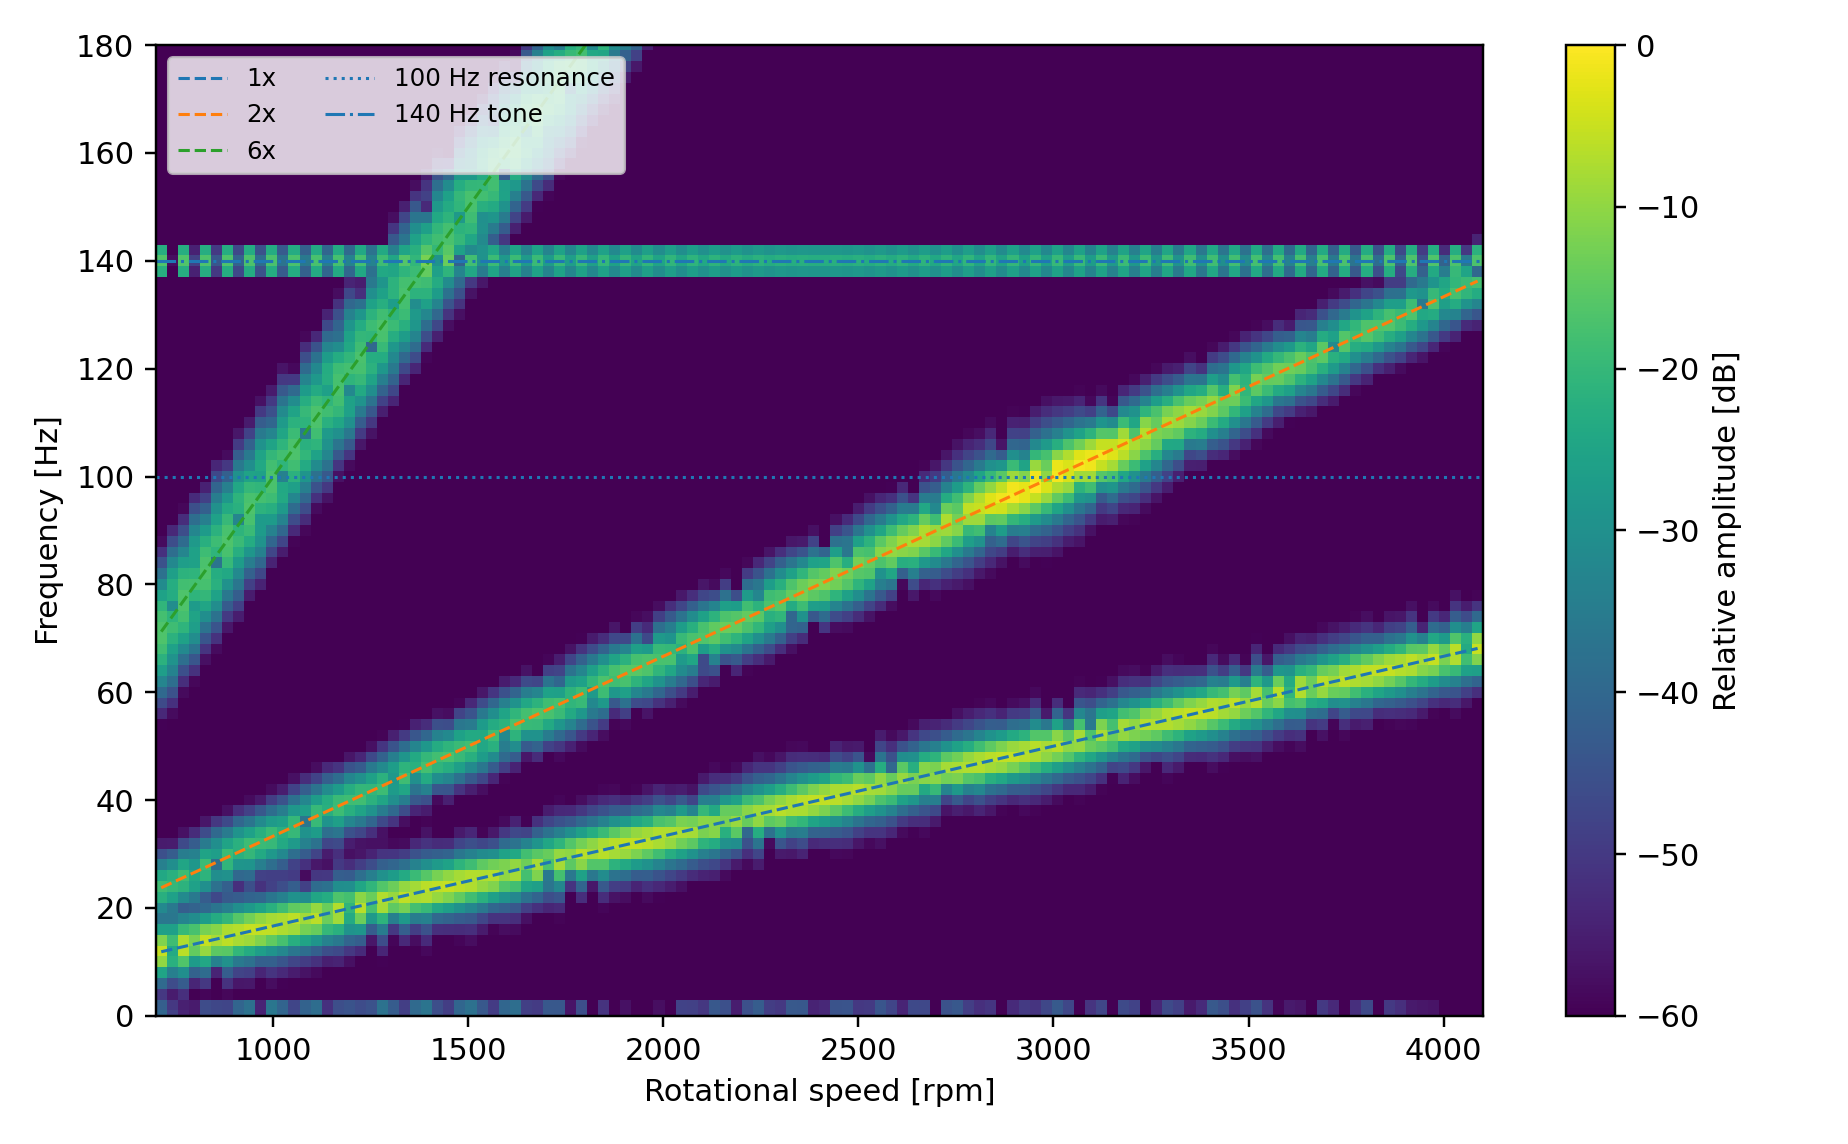
\includegraphics[width=0.92\textwidth]{img/campbell_runup.png}
    \caption{Synthetic response Campbell diagram. The first, second and sixth
    orders rise linearly with speed. The second order is amplified where it
    crosses the $ 100\,\mathrm{Hz} $ resonance, while the stationary
    $ 140\,\mathrm{Hz} $ tone remains horizontal.}
    \label{fig:campbell-runup-example}
\end{figure}


\subsection{Waterfall Representation of the Response Campbell Field}

The response Campbell field in Equation~\eqref{campbell-field-definition} may
also be displayed as a \textbf{waterfall diagram}. No new transform is
performed. Each row of the Campbell field is drawn as an individual spectrum at
its corresponding speed:

\begin{equation}\label{campbell-waterfall-curve}
    \mathcal{W}_b
    =
    \left\{
        \left(f_k,\bar n_b,A(\bar n_b,f_k)\right)
        \;\middle|\;
        k=0,\ldots,N_f-1
    \right\}.
\end{equation}

The frequency axis remains horizontal, the spectra are separated along the
speed axis, and amplitude is shown by the height of each curve. A waterfall is
therefore a three-dimensional perspective view of the same data that a response
Campbell diagram displays by colour or contours. A time waterfall can be formed
in exactly the same manner by replacing speed with block-centre time.

The two views emphasise different properties. A colour map makes ridge geometry,
order lines and weak components easier to compare quantitatively. A waterfall
makes the individual spectra and the growth and decay of resonant peaks more
intuitive. Perspective, curve overlap and the selected viewing angle can,
however, hide weaker components behind stronger curves. Only every few speed
slices are therefore commonly drawn.

When amplitudes are converted to decibels, every slice should use the same global
reference. Normalising each spectrum separately would make every speed slice
appear equally strong and would remove the amplitude increase at a resonance.
The chosen decibel floor also affects the visual appearance but not the
underlying Campbell field.

\begin{python}
import numpy as np
import matplotlib.pyplot as plt


def Plot_Campbell_Waterfall(campbell: dict,
                            maximum_frequency: float | None = None,
                            stride: int = 5,
                            decibel: bool = True,
                            floor_db: float = -60.0):
    """Plot selected speed slices of a response Campbell field."""
    speed_rpm = np.asarray(campbell["speed_rpm"], dtype=float)
    frequency = np.asarray(campbell["frequency_hz"], dtype=float)
    amplitude = np.asarray(campbell["amplitude"], dtype=float)

    if amplitude.shape != (speed_rpm.size, frequency.size):
        raise ValueError("the Campbell field dimensions are inconsistent")
    if stride < 1:
        raise ValueError("stride must be positive")

    if maximum_frequency is None:
        maximum_frequency = frequency[-1]
    frequency_mask = frequency <= maximum_frequency
    frequency_plot = frequency[frequency_mask]
    amplitude_plot = amplitude[:, frequency_mask]

    if decibel:
        reference = np.max(amplitude_plot)
        if reference <= 0.0:
            raise ValueError("the Campbell field contains no positive amplitude")
        minimum_ratio = 10.0**(floor_db / 20.0)
        ordinate = 20.0 * np.log10(
            np.maximum(amplitude_plot / reference, minimum_ratio)
        )
        amplitude_label = "Relative amplitude [dB]"
    else:
        ordinate = amplitude_plot
        amplitude_label = "Peak amplitude"

    figure = plt.figure()
    axis = figure.add_subplot(111, projection="3d")

    rows = list(range(0, speed_rpm.size, stride))
    if rows[-1] != speed_rpm.size - 1:
        rows.append(speed_rpm.size - 1)

    for row in rows:
        speed_line = np.full(frequency_plot.size, speed_rpm[row])
        axis.plot(
            frequency_plot,
            speed_line,
            ordinate[row],
            linewidth=0.8,
        )

    axis.set_xlabel("Frequency [Hz]")
    axis.set_ylabel("Rotational speed [rpm]")
    axis.set_zlabel(amplitude_label)
    figure.tight_layout()
    return figure, axis


Plot_Campbell_Waterfall(
    campbell,
    maximum_frequency=180.0,
    stride=6,
    decibel=True,
)
plt.show()
\end{python}

\begin{figure}[H]
    \centering
    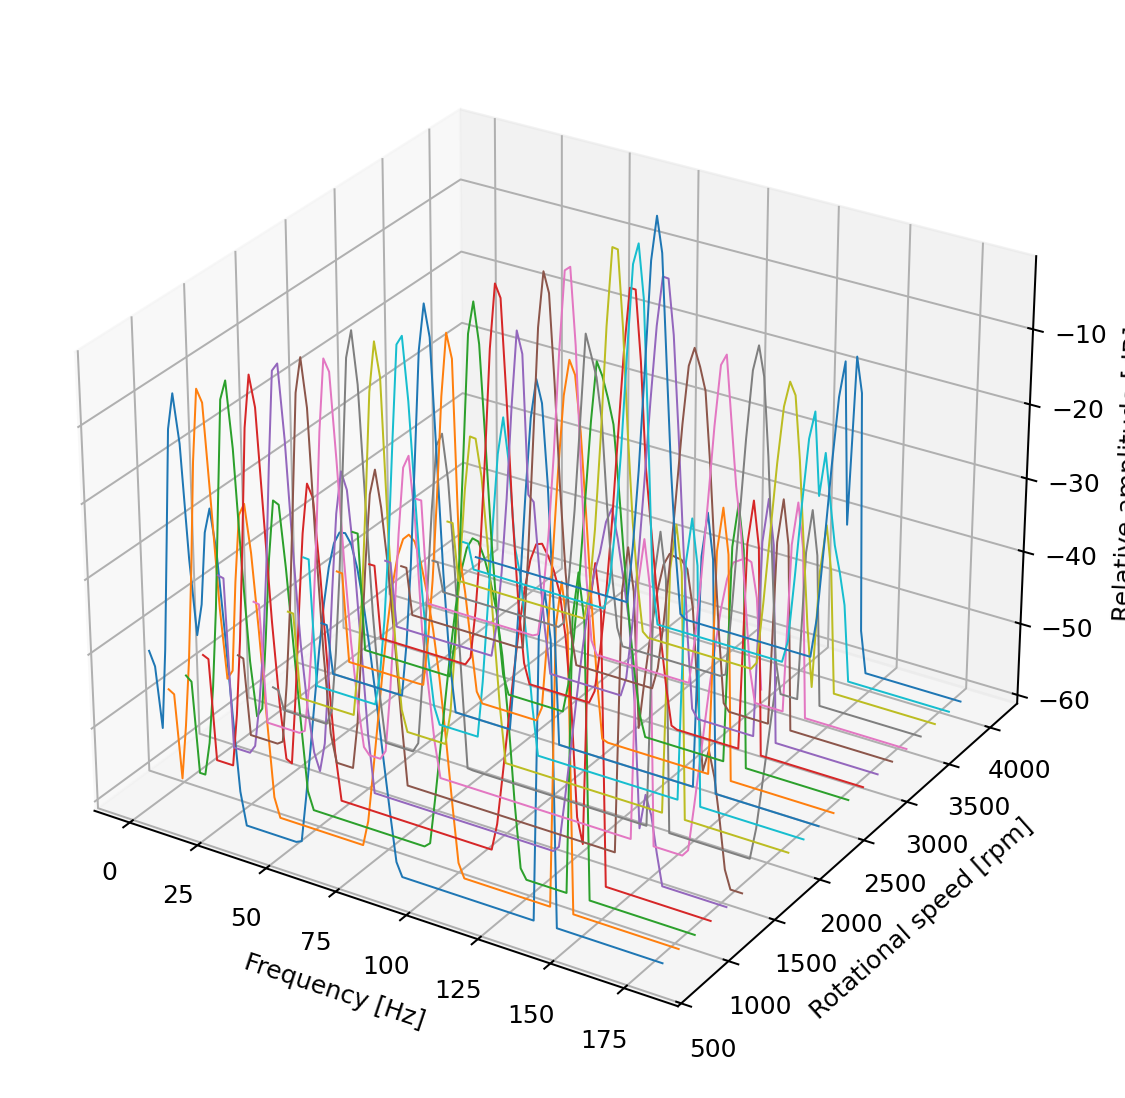
\includegraphics[width=0.92\textwidth]{img/campbell_waterfall_runup.png}
    \caption{Waterfall representation of the synthetic response Campbell field.
    Each line is one spectrum at one rotational speed. The order-related peaks
    move in frequency, while the stationary $140\,\mathrm{Hz}$ component remains
    at the same frequency.}
    \label{fig:campbell-waterfall-runup-example}
\end{figure}

The response Campbell colour map in
Figure~\ref{fig:campbell-runup-example} and the waterfall in
Figure~\ref{fig:campbell-waterfall-runup-example} contain the same spectral
slices. They should not be confused with rainflow cycle counting, which starts
from a load or stress history and answers a fatigue question rather than a
frequency-content question.

\subsection{Order Map Obtained from a Campbell Field}

The order corresponding to frequency $ f $ at speed $ n_{\mathrm{rpm}} $ is:

\begin{equation}\label{frequency-to-order-definition}
    o = \frac{f}{f_{\mathrm{rot}}}
      = \frac{60f}{n_{\mathrm{rpm}}}.
\end{equation}

A Campbell field can therefore be sampled along the frequency curves
$ f=o n_{\mathrm{rpm}}/60 $ to form an order map:

\begin{equation}\label{campbell-to-order-map}
    A_o(n_{\mathrm{rpm}},o)
    = A\left(
        n_{\mathrm{rpm}},
        o\frac{n_{\mathrm{rpm}}}{60}
      \right).
\end{equation}

Because the required frequency usually lies between FFT bins, interpolation is
necessary. Interpolating the complex spectrum retains amplitude and phase more
consistently than separately interpolating magnitude and wrapped phase.

This conversion changes coordinates but does not remove spectral smearing that
already occurred inside the time blocks. It is suitable when speed is nearly
constant within each block. Angular resampling, introduced later, is preferable
for rapid speed changes.

\begin{python}
import numpy as np


def Interpolate_Complex_Spectrum(frequency: np.ndarray,
                                 spectrum: np.ndarray,
                                 target_frequency: np.ndarray) -> np.ndarray:
    """Interpolate a complex spectrum at requested frequencies."""
    frequency = np.asarray(frequency, dtype=float).reshape(-1)
    spectrum = np.asarray(spectrum, dtype=complex).reshape(-1)
    target_frequency = np.asarray(target_frequency, dtype=float).reshape(-1)

    if spectrum.size != frequency.size:
        raise ValueError("spectrum and frequency must have equal length")
    if np.any(np.diff(frequency) <= 0.0):
        raise ValueError("frequency must be strictly increasing")

    result = np.full(target_frequency.size, np.nan + 1.0j * np.nan)

    for index, value in enumerate(target_frequency):
        if value < frequency[0] or value > frequency[-1]:
            continue

        right = np.searchsorted(frequency, value, side="right")
        if right == 0:
            result[index] = spectrum[0]
        elif right == frequency.size:
            result[index] = spectrum[-1]
        else:
            left = right - 1
            fraction = (
                (value - frequency[left])
                / (frequency[right] - frequency[left])
            )
            result[index] = (
                (1.0 - fraction) * spectrum[left]
                + fraction * spectrum[right]
            )

    return result


def Campbell_To_Order_Map(campbell: dict,
                           n_order_bins: int = 401,
                           maximum_order: float | None = None):
    """Interpolate a complex Campbell field onto a common order axis."""
    speed_rpm = np.asarray(campbell["speed_rpm"], dtype=float)
    frequency = np.asarray(campbell["frequency_hz"], dtype=float)
    field = np.asarray(campbell["complex_amplitude"], dtype=complex)

    if np.any(speed_rpm <= 0.0):
        raise ValueError("order conversion requires positive speed")
    if n_order_bins < 2:
        raise ValueError("n_order_bins must be at least two")

    common_limit = frequency[-1] / np.max(speed_rpm / 60.0)
    if maximum_order is None:
        maximum_order = common_limit
    if maximum_order <= 0.0 or maximum_order > common_limit:
        raise ValueError("maximum_order exceeds the common frequency range")

    order = np.linspace(0.0, maximum_order, n_order_bins)
    order_field = np.empty((speed_rpm.size, order.size), dtype=complex)

    for row, speed in enumerate(speed_rpm):
        target_frequency = order * speed / 60.0
        order_field[row] = Interpolate_Complex_Spectrum(
            frequency,
            field[row],
            target_frequency,
        )

    return {
        "speed_rpm": speed_rpm,
        "order": order,
        "complex_amplitude": order_field,
        "amplitude": np.abs(order_field),
    }
\end{python}

In an order map, shaft-synchronous excitations become approximately horizontal.
A speed-independent structural resonance follows:

\begin{equation}
    o_n(n_{\mathrm{rpm}})
    = \frac{60 f_n}{n_{\mathrm{rpm}}},
\end{equation}

and therefore curves downward as speed increases. This is the complementary
view of the frequency--speed Campbell diagram: orders are horizontal and fixed
frequencies are curved.

\begin{python}
import numpy as np
import matplotlib.pyplot as plt


order_map = Campbell_To_Order_Map(
    campbell,
    n_order_bins=481,
    maximum_order=8.0,
)

reference = np.nanmax(order_map["amplitude"])
level_db = 20.0 * np.log10(
    np.maximum(order_map["amplitude"] / reference, 1.0e-6)
)

plt.figure()
plt.pcolormesh(
    order_map["speed_rpm"],
    order_map["order"],
    level_db.T,
    shading="auto",
)
plt.xlabel("Rotational speed [rpm]")
plt.ylabel("Order [-]")
plt.ylim(0.0, 8.0)
plt.colorbar(label="Relative amplitude [dB]")
plt.tight_layout()
plt.show()
\end{python}

\begin{figure}[H]
    \centering
    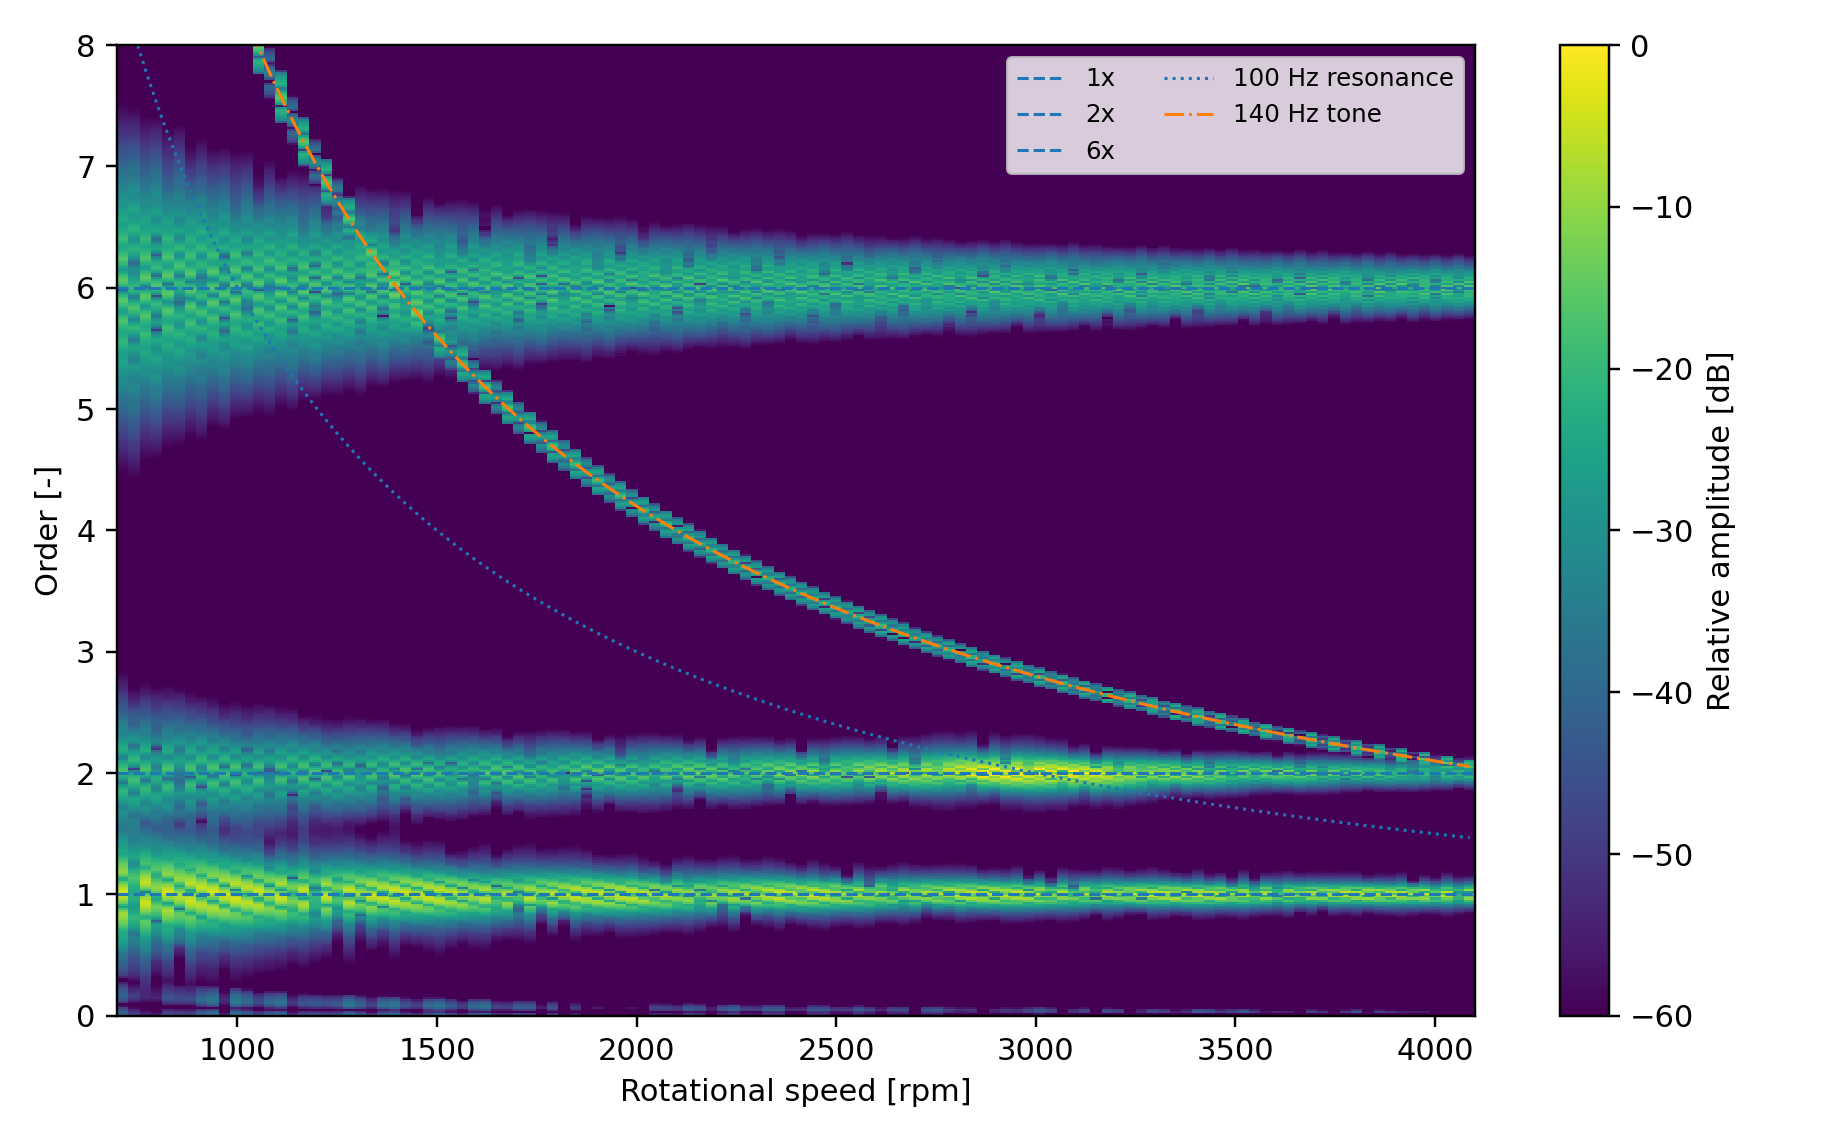
\includegraphics[width=0.92\textwidth]{img/order_map_runup.png}
    \caption{Order map obtained from the synthetic Campbell field. The first,
    second and sixth orders are horizontal. The stationary $ 140\,\mathrm{Hz} $
    component curves towards lower order as speed increases.}
    \label{fig:order-map-runup-example}
\end{figure}

\subsection{Extraction of Individual Order Tracks}

Often the full field is less useful than the amplitude and phase of selected
orders. For each speed slice, the complex spectrum is interpolated at the order
frequency from Equation~\eqref{order-frequency-line}. The resulting complex
track contains both quantities:

\begin{equation}
    a_o(n)=\abs{X_o(n)},
    \qquad
    \varphi_o(n)=\arg X_o(n).
\end{equation}

\begin{python}
import numpy as np


def Extract_Order_Tracks(campbell: dict,
                         orders: np.ndarray) -> dict:
    """Extract complex order tracks from a Campbell field."""
    speed_rpm = np.asarray(campbell["speed_rpm"], dtype=float)
    frequency = np.asarray(campbell["frequency_hz"], dtype=float)
    field = np.asarray(campbell["complex_amplitude"], dtype=complex)
    orders = np.asarray(orders, dtype=float).reshape(-1)

    tracks = np.empty((speed_rpm.size, orders.size), dtype=complex)

    for row, speed in enumerate(speed_rpm):
        target_frequency = orders * speed / 60.0
        tracks[row] = Interpolate_Complex_Spectrum(
            frequency,
            field[row],
            target_frequency,
        )

    return {
        "speed_rpm": speed_rpm,
        "order": orders,
        "complex_amplitude": tracks,
        "amplitude": np.abs(tracks),
        "phase": np.angle(tracks),
    }


tracks = Extract_Order_Tracks(
    campbell,
    orders=np.array([1.0, 2.0, 6.0]),
)
\end{python}

Phase is meaningful only relative to a consistent rotational reference. Speed
obtained from a slowly varying analogue channel may be sufficient for amplitude
tracking but not for absolute order phase. A once-per-revolution tachometer or
encoder reference is required when phase relative to the shaft is important.

\subsection{Angular Resampling for Order Tracking}

During a rapid speed sweep, equal time increments do not correspond to equal
shaft-angle increments. A time-domain sinusoid of constant order is therefore a
chirp. A block FFT assumes approximately stationary frequency and smears the
component if its frequency changes appreciably inside the block.

Order tracking removes this motion by changing the independent variable from
time to rotational angle. The angle is obtained from the rotational speed:

\begin{equation}\label{angle-from-speed-integral}
    \theta(t)
    = \theta_0
    + \int_{t_0}^{t}
      2\pi\frac{n_{\mathrm{rpm}}(\tau)}{60}
      \,\mathrm{d}\tau.
\end{equation}

The response is then interpolated at uniformly spaced angles:

\begin{equation}
    \theta_m=\theta_0+m\Delta\theta,
    \qquad
    x_m^{(\theta)}=x\left(t(\theta_m)\right).
\end{equation}

A component at order $ o $ becomes an ordinary sinusoid in angle:

\begin{equation}
    x^{(\theta)}(\theta)
    = A\cos(o\theta+\varphi).
\end{equation}

The following implementation performs trapezoidal angle integration and linear
interpolation onto a uniform angular grid. It requires monotonically increasing
angle. Data containing a reversal or a prolonged zero-speed interval should be
split into monotonic rotational segments.

\begin{python}
import numpy as np


def Linear_Interpolate_Monotone(x: np.ndarray,
                                y: np.ndarray,
                                x_new: np.ndarray) -> np.ndarray:
    """Linear interpolation for a strictly increasing source coordinate."""
    x = np.asarray(x, dtype=float).reshape(-1)
    y = np.asarray(y).reshape(-1)
    x_new = np.asarray(x_new, dtype=float).reshape(-1)

    if y.size != x.size:
        raise ValueError("x and y must have equal length")
    if np.any(np.diff(x) <= 0.0):
        raise ValueError("x must be strictly increasing")
    if x_new[0] < x[0] or x_new[-1] > x[-1]:
        raise ValueError("x_new must remain inside the source interval")

    result = np.empty(x_new.size, dtype=np.result_type(y, float))

    for index, value in enumerate(x_new):
        right = np.searchsorted(x, value, side="right")
        if right == 0:
            result[index] = y[0]
        elif right == x.size:
            result[index] = y[-1]
        else:
            left = right - 1
            fraction = (value - x[left]) / (x[right] - x[left])
            result[index] = (
                (1.0 - fraction) * y[left]
                + fraction * y[right]
            )

    return result


def Angular_Resample(time: np.ndarray,
                     signal: np.ndarray,
                     speed_rpm: np.ndarray,
                     samples_per_revolution: int):
    """Resample a time signal at uniform shaft-angle increments."""
    time = np.asarray(time, dtype=float).reshape(-1)
    signal = np.asarray(signal, dtype=float).reshape(-1)
    speed_rpm = np.asarray(speed_rpm, dtype=float).reshape(-1)

    if signal.size != time.size or speed_rpm.size != time.size:
        raise ValueError("time, signal and speed_rpm must have equal length")
    if samples_per_revolution < 2:
        raise ValueError("samples_per_revolution must be at least two")

    angle = Rotational_Angle(time, speed_rpm)
    if np.any(np.diff(angle) <= 0.0):
        raise ValueError("rotational angle must be strictly increasing")

    angle_step = 2.0 * np.pi / samples_per_revolution
    first_index = int(np.ceil(angle[0] / angle_step))
    last_index = int(np.floor(angle[-1] / angle_step))
    angle_uniform = (
        np.arange(first_index, last_index + 1) * angle_step
    )

    signal_angle = Linear_Interpolate_Monotone(
        angle,
        signal,
        angle_uniform,
    )
    speed_angle = Linear_Interpolate_Monotone(
        angle,
        speed_rpm,
        angle_uniform,
    )

    return angle_uniform, signal_angle, speed_angle
\end{python}

If the angular signal has $ M $ samples per revolution and a block spans $ R $
revolutions, then:

\begin{equation}
    N_b=MR,
    \qquad
    \Delta o=\frac{1}{R},
    \qquad
    o_{\mathrm{Nyquist}}=\frac{M}{2}.
\end{equation}

Thus the number of revolutions per block controls order resolution, while the
number of samples per revolution controls the highest representable order. This
is the angular-domain counterpart of time-record duration and sample rate.

\begin{python}
import numpy as np


def Angular_Order_Map(time: np.ndarray,
                      signal: np.ndarray,
                      speed_rpm: np.ndarray,
                      samples_per_revolution: int,
                      revolutions_per_block: int,
                      overlap: float = 0.5,
                      duplicate_tolerance_rpm: float = 0.0,
                      resample: int | None = None):
    """Construct an order map after uniform-angle resampling."""
    _, signal_angle, speed_angle = Angular_Resample(
        time,
        signal,
        speed_rpm,
        samples_per_revolution,
    )

    block_size = samples_per_revolution * revolutions_per_block
    if block_size < 2 or block_size & (block_size - 1):
        raise ValueError(
            "samples_per_revolution * revolutions_per_block "
            "must be a power of two"
        )
    if block_size > signal_angle.size:
        raise ValueError("the angular record is shorter than one block")
    if not 0.0 <= overlap < 1.0:
        raise ValueError("overlap must lie in [0, 1)")

    hop_size = max(1, int(round(block_size * (1.0 - overlap))))
    starts = range(0, signal_angle.size - block_size + 1, hop_size)

    index = np.arange(block_size)
    window = 0.5 - 0.5 * np.cos(
        2.0 * np.pi * index / (block_size - 1)
    )
    coherent_gain = np.sum(window) / block_size

    order = (
        np.arange(block_size // 2 + 1)
        / revolutions_per_block
    )
    block_speeds = []
    speed_spreads = []
    spectra = []

    for start in starts:
        stop = start + block_size
        block = signal_angle[start:stop].copy()
        block -= np.mean(block)

        spectrum = FFT_Radix2(block * window)
        complex_amplitude = (
            spectrum[:block_size // 2 + 1]
            / (block_size * coherent_gain)
        )
        complex_amplitude[1:-1] *= 2.0

        local_speed = speed_angle[start:stop]
        block_speeds.append(np.mean(local_speed))
        speed_spreads.append(np.max(local_speed) - np.min(local_speed))
        spectra.append(complex_amplitude)

    block_speeds, spectra, speed_spreads = (
        Sort_And_Average_Speed_Slices(
            np.asarray(block_speeds),
            np.asarray(spectra),
            np.asarray(speed_spreads),
            tolerance_rpm=duplicate_tolerance_rpm,
        )
    )

    if resample is not None:
        if resample < 2:
            raise ValueError("resample must be at least two")
        speed_uniform = np.linspace(
            block_speeds[0],
            block_speeds[-1],
            resample,
        )
        spectra = Interpolate_Field_Rows(
            block_speeds,
            spectra,
            speed_uniform,
        )
        speed_spreads = Interpolate_Field_Rows(
            block_speeds,
            speed_spreads[:, None],
            speed_uniform,
        )[:, 0]
        block_speeds = speed_uniform

    return {
        "speed_rpm": block_speeds,
        "order": order,
        "complex_amplitude": spectra,
        "amplitude": np.abs(spectra),
        "speed_spread_rpm": speed_spreads,
    }
\end{python}

For the synthetic run-up, choosing $ 64 $ samples per revolution and $ 16 $
revolutions per block gives:

\begin{equation}
    N_b=1024,
    \qquad
    \Delta o=0.0625,
    \qquad
    o_{\mathrm{Nyquist}}=32.
\end{equation}

The first, second and sixth orders then remain at fixed order positions despite
the changing speed.

\begin{python}
order_map_angular = Angular_Order_Map(
    time,
    signal,
    speed_rpm,
    samples_per_revolution=64,
    revolutions_per_block=16,
    overlap=0.75,
    resample=120,
)
\end{python}

\subsection{Tachometer Processing and Practical Limitations}

Angular resampling is only as accurate as the estimated angle. Integrating a
noisy speed signal accumulates phase error. A once-per-revolution tachometer
provides discrete angular reference events and prevents long-term drift. An
encoder with several pulses per revolution provides more local information, but
missing or false pulses must be detected before interpolation.

A practical procedure is:

\begin{enumerate}
    \item detect and validate tachometer edges;
    \item assign a known angular increment to consecutive edges;
    \item interpolate angle monotonically between the edges;
    \item resample the response at uniform angular increments;
    \item apply an angular-domain window and FFT;
    \item associate each block with its mean speed and speed spread.
\end{enumerate}

The original time sampling must be high enough for the largest frequency present
at the highest speed. Angular resampling cannot recover a component that was
already aliased in the time-domain acquisition. Conversely, at low speed a fixed
number of angular samples per revolution may correspond to a low effective time
sample rate. Anti-alias filtering and the selected speed range must therefore be
considered together.

If two shafts rotate at different speeds, the stated order always refers to one
chosen reference shaft. A component that is synchronous with another shaft may
appear as a non-integer or speed-dependent order. Gear ratios, slip and variable
transmission ratios should be applied explicitly rather than assuming that every
ridge belongs to the reference shaft.

\subsection{Interpretation and Validation}

A Campbell or order map should be checked against the underlying time and speed
data. Useful validation steps include:

\begin{enumerate}
    \item Verify the FFT frequency bins, amplitude convention and window gain on
        a harmonic of known amplitude.

    \item Plot the speed spread of every block. Broad ridges in blocks with large
        $ \Delta n_b $ may be processing smear rather than physical damping.

    \item Overlay expected order lines and known structural frequencies. A ridge
        should follow the appropriate geometry in both frequency and order views.

    \item Extract selected complex order tracks and compare them with direct
        narrow-band or synchronous calculations.

    \item Process run-up and coast-down separately before deciding whether they
        can be combined.

    \item Confirm that speed sorting, duplicate averaging and optional uniform
        speed rebinning do not alter integrated amplitudes unexpectedly.
\end{enumerate}

The frequency--speed Campbell diagram and the speed--order map are not competing
representations. They emphasize different structures. A constant order is easy
to identify in the order map, while a speed-independent resonance is easy to
identify in the frequency Campbell diagram. Interpreting both views together is
usually more reliable than relying on either one alone.



\section{Rainflow Cycle Counting}

A \textbf{rainflow analysis} is not another representation of a Campbell
field. Campbell and waterfall plots describe how spectral content varies with
speed or time. Rainflow counting operates directly on a scalar load, strain or
stress history and reduces it to fatigue cycles.

\begin{center}
\begin{tabular}{@{}p{0.18\textwidth}p{0.31\textwidth}p{0.39\textwidth}@{}}
\textbf{Method} & \textbf{Coordinates or output} & \textbf{Main purpose} \\
\hline
Response Campbell & speed, frequency and amplitude & rotating-vibration diagnosis \\
Waterfall & stacked spectra versus speed or time & perspective view of spectra \\
Rainflow counting & range, mean and cycle count & fatigue-cycle description
\end{tabular}
\end{center}

The conventional rainflow result does not retain frequency, phase or the exact
time ordering of the cycles. If cycle counts must also be associated with speed,
temperature or another operating state, the record must be divided or each
counted cycle must be linked back to the relevant interval before this
information is discarded.

\subsection{Ranges, Means and Half Cycles}

Let $s(t)$ be a scalar stress history. Consecutive equal values and samples that
are not local extrema are first removed. The remaining reversal sequence is:

\begin{equation}
    r_0,r_1,\ldots,r_{N_r-1}.
\end{equation}

A counted excursion between reversal values $r_a$ and $r_b$ is described by its
range, amplitude and mean:

\begin{equation}\label{rainflow-cycle-quantities}
    \Delta s = \abs{r_b-r_a},
    \qquad
    s_a=\frac{\Delta s}{2},
    \qquad
    s_m=\frac{r_a+r_b}{2}.
\end{equation}

A closed interior cycle has count $c=1$. An unclosed excursion at the beginning
or end of a finite record has count $c=1/2$. Two identical half cycles therefore
contribute the same total count as one full cycle. Whether residual half cycles
should be retained, repeated to close a periodic record or treated by another
record-specific convention must be stated.

Rainflow counting is often explained by imagining rain flowing down a pagoda
roof formed by the rotated stress history. Numerically, a stack of reversals is
more direct. When a new reversal arrives, the two most recent ranges are
compared:

\begin{equation}
    R_{\mathrm{old}}=\abs{r_{j-1}-r_{j-2}},
    \qquad
    R_{\mathrm{new}}=\abs{r_j-r_{j-1}}.
\end{equation}

If $R_{\mathrm{new}}<R_{\mathrm{old}}$, the older excursion remains open. If
$R_{\mathrm{new}}\geq R_{\mathrm{old}}$, the older excursion is closed and
counted. An excursion touching the beginning of the current stack is counted as
a half cycle; an enclosed excursion is counted as a full cycle. After all
reversals have been processed, the adjacent residual excursions are counted as
half cycles.

\subsection{Python Implementation of Rainflow Counting}

The following implementation returns one row per counted cycle. The columns are
cycle range, cycle mean and count. It deliberately retains half cycles rather
than silently forcing the record to be periodic.

\begin{python}
import numpy as np


def Reversal_Points(signal: np.ndarray) -> np.ndarray:
    """Return endpoints and local extrema after removing plateaus."""
    values = np.asarray(signal, dtype=float).reshape(-1)
    if values.size < 2:
        raise ValueError("at least two samples are required")

    compact = [values[0]]
    for value in values[1:]:
        if value != compact[-1]:
            compact.append(value)

    compact = np.asarray(compact)
    if compact.size == 1:
        return compact.copy()

    reversals = [compact[0]]
    for index in range(1, compact.size - 1):
        incoming = compact[index] - compact[index - 1]
        outgoing = compact[index + 1] - compact[index]
        if incoming * outgoing < 0.0:
            reversals.append(compact[index])
    reversals.append(compact[-1])
    return np.asarray(reversals)


def Rainflow_Cycles(signal: np.ndarray) -> np.ndarray:
    """Return rows [range, mean, count] using a reversal stack."""
    reversals = Reversal_Points(signal)
    stack = []
    cycles = []

    for value in reversals:
        stack.append(float(value))

        while len(stack) >= 3:
            old_range = abs(stack[-2] - stack[-3])
            new_range = abs(stack[-1] - stack[-2])

            if new_range < old_range:
                break

            cycle_mean = 0.5 * (stack[-3] + stack[-2])

            if len(stack) == 3:
                if old_range > 0.0:
                    cycles.append([old_range, cycle_mean, 0.5])
                stack.pop(0)
            else:
                if old_range > 0.0:
                    cycles.append([old_range, cycle_mean, 1.0])
                last = stack.pop()
                stack.pop()
                stack.pop()
                stack.append(last)

    for first, second in zip(stack[:-1], stack[1:]):
        cycle_range = abs(second - first)
        if cycle_range > 0.0:
            cycles.append([
                cycle_range,
                0.5 * (first + second),
                0.5,
            ])

    if not cycles:
        return np.empty((0, 3), dtype=float)
    return np.asarray(cycles, dtype=float)


triangular_history = np.array([0.0, 10.0, 0.0])
print(Rainflow_Cycles(triangular_history))
# Two boundary half cycles of range 10; their total count is one.
\end{python}

A constant or monotonic record contains no closed interior cycles. Its total
change appears only as a residual half cycle. This is appropriate because a
single ramp has not completed a load reversal.

\subsection{Rainflow Matrix}

Individual cycles are commonly collected into a two-dimensional histogram. Let
$\rho_i$ be cycle-range bin edges and $\mu_j$ mean-value bin edges. The
rainflow-matrix entry is:

\begin{equation}\label{rainflow-matrix-definition}
    N_{ij}
    =
    \sum_c
    c_c\,
    \mathbf{1}\!\left(\rho_i\leq\Delta s_c<\rho_{i+1}\right)
    \mathbf{1}\!\left(\mu_j\leq s_{m,c}<\mu_{j+1}\right),
\end{equation}

where $c_c$ is $1$ for a full cycle and $1/2$ for a half cycle. Summing the
matrix gives the total number of equivalent full cycles, including the
fractional contribution of residual excursions.

\begin{python}
import numpy as np


def Rainflow_Matrix(cycles: np.ndarray,
                    range_edges: np.ndarray,
                    mean_edges: np.ndarray) -> np.ndarray:
    """Bin rows [range, mean, count] into a rainflow matrix."""
    cycles = np.asarray(cycles, dtype=float)
    range_edges = np.asarray(range_edges, dtype=float).reshape(-1)
    mean_edges = np.asarray(mean_edges, dtype=float).reshape(-1)

    if cycles.ndim != 2 or cycles.shape[1] != 3:
        raise ValueError("cycles must contain [range, mean, count] rows")
    if np.any(np.diff(range_edges) <= 0.0):
        raise ValueError("range_edges must be strictly increasing")
    if np.any(np.diff(mean_edges) <= 0.0):
        raise ValueError("mean_edges must be strictly increasing")

    matrix = np.zeros((range_edges.size - 1, mean_edges.size - 1))

    for cycle_range, cycle_mean, count in cycles:
        range_bin = np.searchsorted(
            range_edges,
            cycle_range,
            side="right",
        ) - 1
        mean_bin = np.searchsorted(
            mean_edges,
            cycle_mean,
            side="right",
        ) - 1

        if cycle_range == range_edges[-1]:
            range_bin = matrix.shape[0] - 1
        if cycle_mean == mean_edges[-1]:
            mean_bin = matrix.shape[1] - 1

        if (0 <= range_bin < matrix.shape[0]
                and 0 <= mean_bin < matrix.shape[1]):
            matrix[range_bin, mean_bin] += count

    return matrix
\end{python}

The example below contains oscillations with changing amplitude and mean value.
Its time history and resulting rainflow matrix are shown together. The matrix
contains cycle counts, not spectral amplitude.

\begin{python}
import numpy as np
import matplotlib.pyplot as plt


time_rf = np.linspace(0.0, 20.0, 4001)
envelope = 65.0 + 20.0 * np.sin(2.0 * np.pi * 0.08 * time_rf)
mean_stress = 25.0 * np.sin(2.0 * np.pi * 0.03 * time_rf)
stress = (
    mean_stress
    + envelope * np.sin(2.0 * np.pi * 1.4 * time_rf)
    + 18.0 * np.sin(2.0 * np.pi * 0.37 * time_rf)
)

cycles = Rainflow_Cycles(stress)
range_edges = np.linspace(0.0, 1.001 * np.max(cycles[:, 0]), 17)
mean_edges = np.linspace(
    np.min(cycles[:, 1]) - 1.0e-9,
    np.max(cycles[:, 1]) + 1.0e-9,
    17,
)
counts = Rainflow_Matrix(cycles, range_edges, mean_edges)

figure, axes = plt.subplots(2, 1)
axes[0].plot(time_rf, stress)
axes[0].set_xlabel("Time [s]")
axes[0].set_ylabel("Stress")

mesh = axes[1].pcolormesh(
    mean_edges,
    range_edges,
    counts,
    shading="flat",
)
axes[1].set_xlabel("Cycle mean")
axes[1].set_ylabel("Cycle range")
figure.colorbar(mesh, ax=axes[1], label="Cycle count")
figure.tight_layout()
plt.show()
\end{python}

\begin{figure}[H]
    \centering
    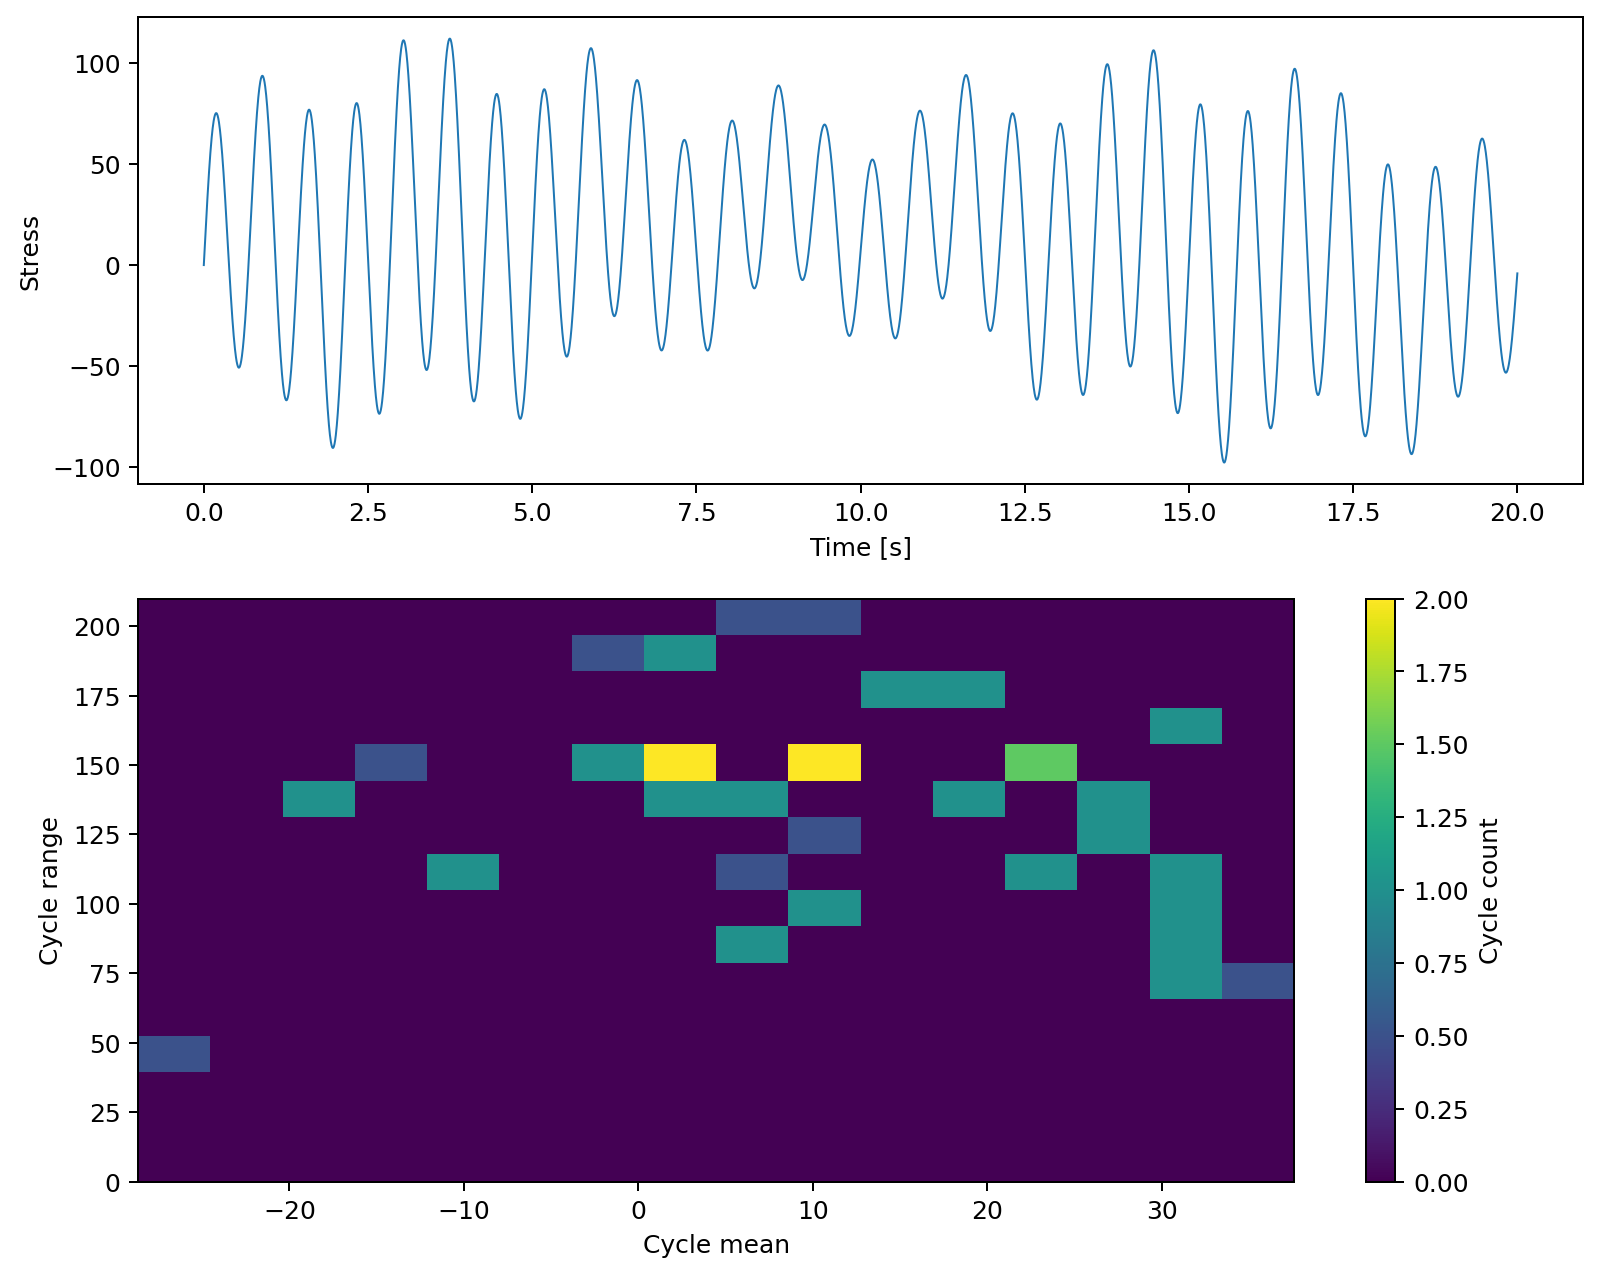
\includegraphics[width=0.92\textwidth]{img/rainflow_counting_example.png}
    \caption{Variable stress history and its rainflow matrix. Each matrix cell
    accumulates full and half cycles having a similar range and mean value. The
    result contains no frequency or rotational-speed coordinate.}
    \label{fig:rainflow-counting-example}
\end{figure}

\subsection{Relation to Fatigue Damage}

Rainflow counting supplies the cycle ranges, means and counts required by a
fatigue model; it does not calculate damage by itself. For a stress-life curve
that assigns an allowable life $N_c$ to each corrected cycle amplitude, linear
Palmgren--Miner accumulation is:

\begin{equation}\label{miner-damage-from-rainflow}
    D=\sum_c\frac{c_c}{N_c}.
\end{equation}

Before looking up $N_c$, a mean-stress correction may be required because two
cycles with the same range but different means need not cause the same damage.
Material data, surface condition, stress concentration, multiaxial state and the
chosen fatigue model remain separate modelling inputs. The rainflow matrix is
therefore an economical description of the load history, not a complete fatigue
assessment.


\section{Power Spectral Density, Cross Spectral Density and Coherence}

\section{Sorting}

\section{Reverse Cuthill-McKee Algorithm for rearranging Sparse matrix}

\section{Topology Optimization}

\section{Generalised Eigenvalue Problem}




